\documentclass[12pt,a4paper,final,twoside,onecolumn,titlepage]{book}

\newcommand*{\plogo}{\fbox{$\mathcal{PL}$}} % Generic publisher logo

%----------------------------------------------------------------------------------------
%	TITLE PAGE
%----------------------------------------------------------------------------------------

\newcommand*{\titleGP}{\begingroup % Create the command for including the title page in the document
\centering % Center all text
\vspace*{\baselineskip} % White space at the top of the page

\rule{\textwidth}{1.6pt}\vspace*{-\baselineskip}\vspace*{2pt} % Thick horizontal line
\rule{\textwidth}{0.4pt}\\[\baselineskip] % Thin horizontal line

{\LARGE Python Concepts \\ The Misunderstood Programming Language}\\[0.2\baselineskip] % Title

\rule{\textwidth}{0.4pt}\vspace*{-\baselineskip}\vspace{3.2pt} % Thin horizontal line
\rule{\textwidth}{1.6pt}\\[\baselineskip] % Thick horizontal line

\scshape % Small caps
Customized for Information Technology Institute \\[\baselineskip] % Tagline(s) or further description
Egypt,  2013\par % Location and year

\vspace*{2\baselineskip} % Whitespace between location/year and editors

Collected by \\[\baselineskip]
{\Large HAITHAM A. EL-GHAREEB \par} % Editor list
{\itshape The University of Mansoura \\ Egypt\par} % Editor affiliation

\vfill % Whitespace between editor names and publisher logo

%\plogo \\[0.3\baselineskip] % Publisher logo
{\large helghareeb@mans.edu.eg \\ http://www.helghareeb.me}\par % Publisher
{\scshape 2013} \\[0.3\baselineskip] % Year published

\endgroup}

\usepackage[export]{adjustbox}

\usepackage{makeidx}
\usepackage[utf8]{inputenc} %File encoding
\usepackage[T1]{fontenc} % Use EC fonts
\usepackage{ae} % Fonts for PDF files
\usepackage{textcomp} % Text-Companion-Symbols (e. g. \texteuro)
\usepackage[english]{babel} % Language selection
\usepackage{lmodern} % Latin Modern

\usepackage{pdfpages}

%New Section Added for Coding
\usepackage{amsmath}
\usepackage{algorithm2e}
\usepackage{amsfonts}
\usepackage{amssymb}
\usepackage{graphicx}
\usepackage{natbib}
\usepackage{listings}
\usepackage{color}
\usepackage{textcomp}
\usepackage{multirow}
\definecolor{listinggray}{gray}{0.9}
\definecolor{lbcolor}{rgb}{0.9,0.9,0.9}
\lstset{
	backgroundcolor=\color{white},
	tabsize=4,
	rulecolor=,
	language=Python,
        basicstyle=\scriptsize,
        upquote=true,
        aboveskip={1.5\baselineskip},
        columns=fixed,
        showstringspaces=false,
        extendedchars=true,
        breaklines=true,
        prebreak = \raisebox{0ex}[0ex][0ex]{\ensuremath{\hookleftarrow}},
        frame=single,
        showtabs=false,
        showspaces=false,
        showstringspaces=false,
        identifierstyle=\ttfamily,
        keywordstyle=\color[rgb]{0,0,1},
        commentstyle=\color[rgb]{0.133,0.545,0.133},
        stringstyle=\color[rgb]{0.627,0.126,0.941},
}

%End of New Section Added for Coding

\usepackage[english]{translator}
%Load the package
\usepackage[
nonumberlist, %do not show page numbers
acronym,      %generate acronym listing
toc,          %show listings as entries in table of contents
section]      %use section level for toc entries
{glossaries}

\usepackage{hyperref}

%Added on March 20, 2013 for fitting figures within Text Boundaries
\usepackage[export]{adjustbox}
\usepackage{tabularx}

%This Package is used for Margins
\usepackage[margin=3.0cm]{geometry}

%Added on March 20, 2013 for fitting figures within Text Boundaries
\usepackage[export]{adjustbox}
\usepackage{tabularx}

%This Package is used for Margins
\usepackage[margin=3.0cm]{geometry}

%Generate a list of symboles
\newglossary[slg]{symbolslist}{syi}{syg}{List of symbols}

%Remove the dot at the end of glossary descriptions
\renewcommand*{\glspostdescription}{}

%Activate glossary commands
\makeglossaries

%These commands sort the lists
%makeindex -s filename.ist -t filename.alg -o filename.acr filename.acn
%makeindex -s filename.ist -t filename.glg -o filename.gls filename.glo
%makeindex -s filename.ist -t filename.slg -o filename.syi filename.syg

%Some entries for the list of symbols
\newglossaryentry{symb:Pi}{
name=$\pi$,
description={A mathematical constant whose value is the ratio of any circle's circumference to its diameter.},
sort=symbolpi, type=symbolslist
}


%Some acronyms
%\newacronym{AEHS}{AEHS}{Adaptive Educational Hypermedia Systems}

%An acronym with a glossary entry
%\newacronym{ADL}{ADL}{Advanced Distributed Learning\protect\glsadd{glos:ADL}}

%Some glossary terms
\newglossaryentry{glos:ADL}{name={ADL}, description = {ADL: Advanced Distributed Learning, established in 1997 to standardize and modernize training and education management and delivery. The Department of Defense (DoD) Office oversees the initiative. http://www.adlnet.gov}}


\author{Haitham A. El-Ghareeb, Ph.D. \\ \texttt{helghareeb@mans.edu.eg}}
\title{Associate Professor}
\date{\today}

\makeindex


\begin{document}
\frontmatter

%\maketitle
%\pagestyle{empty} % Removes page numbers

\thispagestyle{empty}
\titleGP % This command includes the title page


\cleardoublepage
\thispagestyle{empty}
\begin{center}
-= To my Family =- \\
\textit{Haitham A. El-Ghareeb, Ph.D.}
\end{center}

\begin{flushright}
March, 2013
\end{flushright}

\cleardoublepage
\phantomsection
\chapter{Acknowledgment}
%\addcontentsline{toc}{chapter}{Acknowledgment}
\thispagestyle{empty}
\paragraph*{
First and foremost, I thank ALLAH for giving me incentive to go on and finish this work, and every other work have been finished and giving me glimpses of heavenly hope in the darkest times.}

\paragraph*{I would like to thank Eng. Ayman Lotfy for the cooperation, generousity, and support.}

\paragraph*{My Family, you are the people whom without I could not have continued the journey to the day I witness this book alive. Thanks for always being there to support me, every single moment, with everything you can, when I was about to lose hope and trust in me being able to continue through the darkness, trying to reach the goal through long nights of mess, you were there, through long distances you were pushing me forward by your support, encouragement, guidance, and help. Thanks to ALLAH, I am really blessed with amazing family like you. I Love You all!}

\thispagestyle{empty}

\begin{flushright}
\textit{Haitham A. El-Ghareeb} \\
March, 2013
\end{flushright}

\cleardoublepage
\phantomsection
\tableofcontents

\chapter{Preface}
%\addcontentsline{toc}{chapter}{Preface}

\mainmatter

\chapter{Teach yourself Programming in 10 Years}

By: Peter Norvig

\section{Why is everyone in such a rush?}

Walk into any bookstore, and you'll see how to Teach Yourself Java in 7 Days alongside endless variations offering to teach Visual Basic, Windows, the Internet, and so on in a few days or hours. I did the following power search at Amazon.com: pubdate: after 1992 and title: days and (title: learn or title: teach yourself)
and got back 248 hits. The first 78 were computer books (number 79 was Learn Bengali in 30 days). I replaced "days" with "hours" and got remarkably similar results: 253 more books, with 77 computer books followed by Teach Yourself Grammar and Style in 24 Hours at number 78. Out of the top 200 total, 96\% were computer books.
The conclusion is that either people are in a big rush to learn about computers, or that computers are somehow fabulously easier to learn than anything else. There are no books on how to learn Beethoven, or Quantum Physics, or even Dog Grooming in a few days. Felleisen et al. give a nod to this trend in their book How to Design Programs, when they say "Bad programming is easy. Idiots can learn it in 21 days, even if they are dummies.

Let's analyze what a title like Learn C++ in Three Days could mean:
\begin{itemize}
\item Learn: In 3 days you won't have time to write several significant programs, and learn from your successes and failures with them. You won't have time to work with an experienced programmer and understand what it is like to live in a C++ environment. In short, you won't have time to learn much. So the book can only be talking about a superficial familiarity, not a deep understanding. As Alexander Pope said, a little learning is a dangerous thing.
\item C++: In 3 days you might be able to learn some of the syntax of C++ (if you already know another language), but you couldn't learn much about how to use the language. In short, if you were, say, a Basic programmer, you could learn to write programs in the style of Basic using C++ syntax, but you couldn't learn what C++ is actually good (and bad) for. So what's the point? Alan Perlis once said: "A language that doesn't affect the way you think about programming, is not worth knowing". One possible point is that you have to learn a tiny bit of C++ (or more likely, something like JavaScript or Flash's Flex) because you need to interface with an existing tool to accomplish a specific task. But then you're not learning how to program; you're learning to accomplish that task.
\item in Three Days: Unfortunately, this is not enough, as the next section shows.
\end{itemize}

\section{Teach Yourself Programming in Ten Years}
Researchers (Bloom (1985), Bryan \& Harter (1899), Hayes (1989), Simmon \& Chase (1973)) have shown it takes about ten years to develop expertise in any of a wide variety of areas, including chess playing, music composition, telegraph operation, painting, piano playing, swimming, tennis, and research in neuropsychology and topology. The key is deliberative practice: not just doing it again and again, but challenging yourself with a task that is just beyond your current ability, trying it, analyzing your performance while and after doing it, and correcting any mistakes. Then repeat. And repeat again. There appear to be no real shortcuts: even Mozart, who was a musical prodigy at age 4, took 13 more years before he began to produce world-class music. In another genre, the Beatles seemed to burst onto the scene with a string of \#1 hits and an appearance on the Ed Sullivan show in 1964. But they had been playing small clubs in Liverpool and Hamburg since 1957, and while they had mass appeal early on, their first great critical success, Sgt. Peppers, was released in 1967. Malcolm Gladwell reports that a study of students at the Berlin Academy of Music compared the top, middle, and bottom third of the class and asked them how much they had practiced:
Everyone, from all three groups, started playing at roughly the same time - around the age of five. In those first few years, everyone practised roughly the same amount - about two or three hours a week. But around the age of eight real differences started to emerge. The students who would end up as the best in their class began to practise more than everyone else: six hours a week by age nine, eight by age 12, 16 a week by age 14, and up and up, until by the age of 20 they were practising well over 30 hours a week. By the age of 20, the elite performers had all totalled 10,000 hours of practice over the course of their lives. The merely good students had totalled, by contrast, 8,000 hours, and the future music teachers just over 4,000 hours.
So it may be that 10,000 hours, not 10 years, is the magic number. (Henri Cartier-Bresson (1908-2004) said "Your first 10,000 photographs are your worst," but he shot more than one an hour.) Samuel Johnson (1709-1784) thought it took even longer: "Excellence in any department can be attained only by the labor of a lifetime; it is not to be purchased at a lesser price." And Chaucer (1340-1400) complained "the lyf so short, the craft so long to lerne." Hippocrates (c. 400BC) is known for the excerpt "ars longa, vita brevis", which is part of the longer quotation "Ars longa, vita brevis, occasio praeceps, experimentum periculosum, iudicium difficile", which in English renders as "Life is short, [the] craft long, opportunity fleeting, experiment treacherous, judgment difficult." Although in Latin, ars can mean either art or craft, in the original Greek the word "techne" can only mean "skill", not "art".

\section{So You Want to be a Programmer}

Here's my recipe for programming success:
\begin{enumerate}
\item Get interested in programming, and do some because it is fun. Make sure that it keeps being enough fun so that you will be willing to put in your ten years/10,000 hours.
\item Program. The best kind of learning is learning by doing. To put it more technically, "the maximal level of performance for individuals in a given domain is not attained automatically as a function of extended experience, but the level of performance can be increased even by highly experienced individuals as a result of deliberate efforts to improve." (p. 366) and "the most effective learning requires a well-defined task with an appropriate difficulty level for the particular individual, informative feedback, and opportunities for repetition and corrections of errors." (p. 20-21) The book Cognition in Practice: Mind, Mathematics, and Culture in Everyday Life is an interesting reference for this viewpoint.
\item Talk with other programmers; read other programs. This is more important than any book or training course.
\item If you want, put in four years at a college (or more at a graduate school). This will give you access to some jobs that require credentials, and it will give you a deeper understanding of the field, but if you don't enjoy school, you can (with some dedication) get similar experience on your own or on the job. In any case, book learning alone won't be enough. "Computer science education cannot make anybody an expert programmer any more than studying brushes and pigment can make somebody an expert painter" says Eric Raymond, author of The New Hacker's Dictionary. One of the best programmers I ever hired had only a High School degree; he's produced a lot of great software, has his own news group, and made enough in stock options to buy his own nightclub.
\item Work on projects with other programmers. Be the best programmer on some projects; be the worst on some others. When you're the best, you get to test your abilities to lead a project, and to inspire others with your vision. When you're the worst, you learn what the masters do, and you learn what they don't like to do (because they make you do it for them).
\item Work on projects after other programmers. Understand a program written by someone else. See what it takes to understand and fix it when the original programmers are not around. Think about how to design your programs to make it easier for those who will maintain them after you.
\item Learn at least a half dozen programming languages. Include one language that supports class abstractions (like Java or C++), one that supports functional abstraction (like Lisp or ML), one that supports syntactic abstraction (like Lisp), one that supports declarative specifications (like Prolog or C++ templates), one that supports coroutines (like Icon or Scheme), and one that supports parallelism (like Sisal).
\item Remember that there is a "computer" in "computer science". Know how long it takes your computer to execute an instruction, fetch a word from memory (with and without a cache miss), read consecutive words from disk, and seek to a new location on disk. (Answers here.)
\item Get involved in a language standardization effort. It could be the ANSI C++ committee, or it could be deciding if your local coding style will have 2 or 4 space indentation levels. Either way, you learn about what other people like in a language, how deeply they feel so, and perhaps even a little about why they feel so.
\item Have the good sense to get off the language standardization effort as quickly as possible.
\end{enumerate}

With all that in mind, its questionable how far you can get just by book learning. Before my first child was born, I read all the How To books, and still felt like a clueless novice. 30 Months later, when my second child was due, did I go back to the books for a refresher? No. Instead, I relied on my personal experience, which turned out to be far more useful and reassuring to me than the thousands of pages written by experts.
Fred Brooks, in his essay No Silver Bullet identified a three-part plan for finding great software designers:
\begin{itemize}
\item Systematically identify top designers as early as possible.
\item Assign a career mentor to be responsible for the development of the prospect and carefully keep a career file.
\item Provide opportunities for growing designers to interact and stimulate each other.
\end{itemize}
This assumes that some people already have the qualities necessary for being a great designer; the job is to properly coax them along. Alan Perlis put it more succinctly: "Everyone can be taught to sculpt: Michelangelo would have had to be taught how not to. So it is with the great programmers". Perlis is saying that the greats have some internal quality that transcends their training. But where does the quality come from? Is it innate? Or do they develop it through diligence? As Auguste Gusteau (the fictional chef in Ratatouille) puts it, "anyone can cook, but only the fearless can be great." I think of it more as willingness to devote a large portion of one's life to deliberative practice. But maybe fearless is a way to summarize that. Or, as Gusteau's critic, Anton Ego, says: "Not everyone can become a great artist, but a great artist can come from anywhere."
So go ahead and buy that Java/Ruby/Javascript/PHP book; you'll probably get some use out of it. But you won't change your life, or your real overall expertise as a programmer in 24 hours, days, or even weeks. How about working hard to continually improve over 24 months? Well, now you're starting to get somewhere...

\chapter{Programming Languages Are Not The Same}
Programming languages are used for controlling the behavior of a machine (often a computer). Like natural languages, programming languages conform to rules for syntax and semantics. There are thousands of programming languages and new ones are created every year. Few languages ever become sufficiently popular that they are used by more than a few people, but professional programmers may use dozens of languages in a career. So, not to get lost between all those programming languages, there are main things we need to discuss in Programming Languages, and comparison between them.
\section{Basis for Comparing Programming Languages}
\subsection{Object Orientation}
Many languages claim to be Object-Oriented. While the exact definition of the term is highly variable, there are several qualities that most will agree an Object-Oriented language should have:
\begin{itemize}
\item Encapsulation/Information Hiding
\item Inheritance
\item Polymorphism/Dynamic Binding
\item All pre-defined types are Objects
\item All operations performed by sending messages to Objects
\item All user-defined types are Objects
\end{itemize}
A language is considered to be a "pure" Object-Oriented languages if it satisfies all of these qualities. A "hybrid" language may support some of these qualities, but not all. In particular, many languages support the first three qualities, but not the final three.

\subsection{Static vs. Dynamic Typing}
The debate between static and dynamic typing has raged in Object-Oriented circles for many years with no clear conclusion. Proponents of dynamic typing contend that it is more flexible and allows for increased productivity. Those who prefer static typing argue that it enforces safer, more reliable code, and increases efficiency of the resulting product.

Statically-typed language requires a very well-defined type system in order to remain as flexible as its dynamically-typed counterparts. Without the presence of genericity (templates) and multiple type inheritance, a static type system may severely inhibit the flexibility of a language. In addition, the presence of "casts" in a language can undermine the ability of the compiler to enforce type constraints.

A dynamic type system doesn't require variables to be declared as a specific type. Any variable can contain any value or object. In many cases this can make the software more flexible and amenable to change. However, care must be taken that variables hold the expected kind of object. Typically, if a variable contains an object of a different type than a user of the object expects, some sort of "message not understood" error is raised at run-time. Users of dynamically-typed languages claim that this type of error is infrequent in practice.

Statically-typed languages require that all variables are declared with a specific type. The compiler will then ensure that at any given time the variable contains only an object compatible with that type. (We say "compatible with that type" rather than "exactly that type" since the inheritance relationship enables subtyping, in which a class that inherits from another class is said to have an IS-A relationship with the class from which it inherits, meaning that instances of the inheriting class can be considered to be of a compatible type with instances of the inherited class.) By enforcing the type constraint on objects contained or referred to by the variable, the compiler can ensure a "message not understood" error can never occur at run-time. On the other hand, a static type system can hinder evolution of software in some circumstances. For example, if a method takes an object as a parameter, changing the type of the object requires changing the signature of the method so that it is compatible with the new type of the object being passed. If this same object is passed to many such methods, all of them must be updated accordingly, which could potentially be an arduous task. One must remember, though, that this ripple effect could occur even a dynamically-typed language. If the type of the object is not what it was originally expected to be, it may not understand the messages being sent to it. Perhaps even worse is that it could understand the message but interpret it in a way not compatible with the semantics of the calling method. A statically-typed language can flag these errors at compilation-time, pointing out the precise locations of potential errors. A user of a dynamically-typed language must rely on extensive testing to ensure that all improper uses of the object are tracked down.

\subsection{Generic Classes}
Generic classes, and more generally parametric type facilities, refer to the ability to parameterize a class with specific data types. A common example is a stack class that is parameterized by the type of elements it contains. This allows the stack to simultaneously be compile-time type safe and yet generic enough to handle any type of elements.

The primary benefit of parameterized types is that it allows statically typed languages to retain their compile-time type safety yet remain nearly as flexible as dynamically typed languages. Dynamically typed languages do not need parameterized types in order to support generic programming. Types are checked at run-time and thus dynamically typed languages support generic programming inherently.

\subsection{Inheritence}
Inheritance is the ability for a class or object to be defined as an extension or specialization of another class or object. Most object-oriented languages support class-based inheritance, while others such as SELF and JavaScript support object-based inheritance. A few languages, notably Python and Ruby, support both class- and object-based inheritance, in which a class can inherit from another class and individual objects can be extended at run time with the capabilities of other objects. 

Though there are identified and classified as many as 17 different forms of inheritance. Even so, most languages provide only a few syntactic constructs for inheritance which are general enough to allow inheritance to be used in many different ways. The most important distinction that can be made between various languages' support for inheritance is whether it supports single or multiple inheritance. Multiple inheritance is the ability for a class to inherit from more than one super (or base) class. For example, an application object called PersistentShape might inherit from both GraphicalObject and PersistentObject in order to be used as both a graphical object that can be displayed on the screen as well as a persistent object that can be stored in a database.

Multiple inheritance would appear to be an essential feature for a language to support for cases such as the above when two or more distinct hierarchies must be merged into one application domain. However, there are other issues to consider before making such an assertion.

First, we must consider that multiple inheritance introduces some complications into a programming language supporting it. Issues such as name clashes and ambiguities introduced in the object model must be resolved by the language in order for multiple inheritance and this leads to additional complexity in the language. 

Next, we must distinguish between implementation inheritance and interface/subtype inheritance. Subtype inheritance (also known loosely as interface inheritance) is the most common form of inheritance, in which a subclass is considered to be a subtype of its super class, commonly referred to as an IS-A relationship. What this means is that the language considers an object to conform to the type of its class or any of its super classes. For example, a Circle IS-A Shape, so anywhere a Shape is used in a program, a Circle may be used as well. This conformance notion is only applicable to statically typed languages since it is a feature used by the compiler to determine type correctness.

Implementation inheritance is the ability for a class to inherit part or all of its implementation from another class. For example, a Stack class that is implemented using an array might inherit from an Array class in order to define the Stack in terms of the Array. In this way, the Stack class could use any features from the Array to support its own implementation. With pure implementation inheritance, the fact that the Stack inherits its implementation from Array would not be visible to code using the Stack; the inheritance would be strictly an implementation matter. 

Returning to the issue of multiple inheritance, we can see that a language's support for multiple inheritance is not a boolean condition; a language can support one or more different forms of multiple inheritance in the same way it can support different forms of single inheritance (e.g. implementation and subtype inheritance). 

\subsection{Feature Renaming}
Feature renaming is the ability for a class or object to rename one of its features (a term used to collectively refer to attributes and methods) that it inherited from a super class. There are two important ways in which this can be put to use:
\begin{itemize}
\item Provide a feature with a more natural name for its new context
\item Resolve naming ambiguities when a name is inherited from multiple inheritance paths
\end{itemize}

\subsection{Method Overloading}
Method overloading (also referred to as parametric polymorphism) is the ability for a class, module, or other scope to have two or more methods with the same name. Calls to these methods are disambiguated by the number and/or type of arguments passed to the method at the call site. For example, a class may have multiple print methods, one for each type of thing to be printed. The alternative to overloading in this scenario is to have a different name for each print method, such as print\_string and print\_integer.

\subsection{Operator Overloading}
Operator overloading is the ability for a programmer to define an operator (such as +, or *) for user-defined types. This allows the operator to be used in infix, prefix, or postfix form, rather than the standard functional form. For example, a user-defined Matrix type might provide a * infix operator to perform matrix multiplication with the familiar notation: matrix1 * matrix2 .

Some (correctly) consider operator overloading to be mere syntactic "sugar" rather than an essential feature, while others (also correctly) point to the need for such syntactic sugar in numerical and other applications. Both points are valid, but it is clear that, when used appropriately, operator overloading can lead to much more readable programs. When abused, it can lead to cryptic, obfuscated code. Consider that in the presence of operator overloading, it may not be clear whether a given operator is built in to the language or defined by the user. For any language that supports operator overloading, two things are necessary to alleviate such obfuscation:

All operations must be messages to objects, and thus all operators are always method calls.
Operators must have an equivalent functional form, so that using the operator as a method call will behave precisely the same as using it in infix, prefix, or postfix form.

\subsection{Higher Order Functions \& Lexical Closures}
Higher order functions are, in the simplest sense, functions that can be treated as if they were data objects. In other words, they can be bound to variables (including the ability to be stored in collections), they can be passed to other functions as parameters, and they can be returned as the result of other functions. Due to this ability, higher order functions may be viewed as a form of deferred execution, wherein a function may be defined in one context, passed to another context, and then later invoked by the second context. This is different from standard functions in that higher order functions represent anonymous lambda functions, so that the invoking context need not know the name of the function being invoked.

Lexical closures (also known as static closures, or simply closures) take this one step further by bundling up the lexical (static) scope surrounding the function with the function itself, so that the function carries its surrounding environment around with it wherever it may be used. This means that the closure can access local variables or parameters, or attributes of the object in which it is defined, and will continue to have access to them even if it is passed to another module outside of its scope.

\subsection{Garbage Collection}
Garbage collection is a mechanism allowing a language implementation to free memory of unused objects on behalf of the programmer, thus relieving the burden on the programmer to do so. The alternative is for the programmer to explicitly free any memory that is no longer needed. There are several strategies for garbage collection that exist in various language implementations.
\subsubsection{Reference Counting}
Reference counting is the simplest scheme and involves the language keeping track of how many references there are to a particular object in memory, and deleting that object when that reference count becomes zero. This scheme, although it is simple and deterministic, is not without its drawbacks, the most important being its inability to handle cycles. Cycles occur when two objects reference each other, and thus there reference counts will never become zero even if neither object is referenced by any other part of the program.
\subsubsection{Mark and Sweep}
"Mark and sweep" garbage collection is another scheme that overcomes this limitation. A mark and sweep garbage collector works in a two phase process, known as the mark phase and the sweep phase. The mark phase works by first starting at the "root" objects (objects on the stack, global objects, etc.), marking them as live, and recursively marking any objects referenced from them. These marked objects are the set of live objects in program, and any objects that were not marked in this phase are unreferenced and therefore candidates for collection. In the sweep phase, any objects in memory that were not marked as live by the mark phase are deleted from memory. The primary drawback of mark and sweep collection is that it is non-deterministic, meaning that objects are deleted at an unspecified time during the execution of the program. This is the most common form of garbage collection.
\subsubsection{Generational}
Generational garbage collection works in a similar fashion to mark and sweep garbage collection, except it capitalizes on the statistical probability that objects that have been alive the longest tend to stay alive longer than objects that were newly created. Thus a generational garbage collector will divide objects into "generations" based upon how long they've been alive. This division can be used to reduce the time spent in the mark and sweep phases because the oldest generation of objects will not need to be collected as frequently. Generational garbage collectors are not as common as the other forms.

\subsection{Uniform Access}
The Uniform Access Principle, states that "All services offered by a module should be available through a uniform notation, which does not betray whether they are implemented through storage or through computation." It is described further with "Although it may at first appear just to address a notational issue, the Uniform Access principle is in fact a design rule which influences many aspects of object-oriented design and the supporting notation. It follows from the Continuity criterion; you may also view it as a special case of Information Hiding."

Say that \texttt{teach} is a feature of a class named \texttt{Professor}. For languages that do not support the Uniform Access Principle, the notation used to access \texttt{teach} differs depending on whether it is an attribute (storage) or a function (computation). For example, in Java we would use \texttt{Professor.teach} if it were an attribute, but we would use \texttt{Professor.teach()} if it were a function. Having this notational difference means that users of \texttt{Professor} are exposed to unnecessary implementation details and are tightly coupled to \texttt{Professor}. If \texttt{teach} is changed from attribute to method (or vice versa), then any users of \texttt{Professor} must also be changed.

The Uniform Access Principle seeks to eliminate this needless coupling. A language supporting the Uniform Access Principle does not exhibit any notational differences between accessing a feature regardless of whether it is an attribute or a function. Thus, in our earlier example, access to bar would always be in the form of foo.bar, regardless of how bar is implemented. This makes clients of Foo more resilient to change.

\subsection{Class Variables/Methods}
Class variables and methods are owned by a class, and not any particular instance of a class. This means that for however many instances of a class exist at any given point in time, only one copy of each class variable/method exists and is shared by every instance of the class.

\subsection{Reflection}
Reflection is the ability for a program to determine various pieces of information about an object at run-time. This includes the ability to determine the type of the object, its inheritance structure, and the methods it contains, including the number and types of parameters and return types. It might also include the ability for determining the names and types of attributes of the object. Most object-oriented languages support some form of reflection.

\subsection{Access Control}
Access control refers to the ability for a modules implementation to remain hidden behind its public interface. Access control is closely related to the encapsulation/information hiding principle of object-oriented languages. For example, a class \texttt{Professor} may have methods such as \texttt{name} and \texttt{email}, that return the professor's name and e-mail address respectively. How these methods work is an implementation detail that should not be available to users of the \texttt{Person} class. These methods may, for example, connect to a database to retrieve the values. The database connection code that is used to do this is not relevant to client code and should not be exposed. Language-enforced access control allows us to enforce this.
Most object-oriented languages provide at least two levels of access control: public and protected. Protected features are not available outside of the class in which they are contained, except for subclasses. Some languages, notably Java and C++, provide a third level of access control known as "private". Private features are not available outside of the class in which they are declared, even for subclasses. Note, however, that this means that objects of a particular class can access the private features of other objects of that same class. Java provides a fourth level of, known as "package private" access control which allows other classes in the same package to access such features.

\subsection{Design by Contract}
Design by Contract (DBC) is the ability to incorporate important aspects of a specification into the software that is implementing it. The most important features of DBC are:
\begin{itemize}
\item Pre-conditions, which are conditions that must be true before a method is invoked
\item Post-conditions, which are conditions guaranteed to be true after the invocation of a method
\item Invariants, which are conditions guaranteed to be true at any stable point during the lifetime of an object
\end{itemize}
There is much more to DBC than these simple facilities, including the manner in which pre-conditions, post-conditions, and invariants are inherited. However, at least these facilities must be present to support the central notions of DBC.

\subsection{Multithreading}
Multithreading is the ability for a single process to process two or more tasks concurrently. (We say concurrently rather than simultaneously because, in the absence of multiple processors, the tasks cannot run simultaneously but rather are interleaved in very small time slices and thus exhibit the appearance and semantics of concurrent execution.) The use of multithreading is becoming increasingly more common as operating system support for threads has become near ubiquitous.

\subsection{Regular Expressions}
Regular expressions are pattern matching constructs capable of recognizing the class of languages known as regular languages. They are frequently used for text processing systems as well as for general applications that must use pattern recognition for other purposes. Libraries with regular expression support exist for nearly every language, however it has become increasingly important for a language to support regular expressions natively. This allows tighter integration with the rest of the language and allows more convenient syntax for use of regular expressions. 

\subsection{Pointer Arithmetic}
Pointer arithmetic is the ability for a language to directly manipulate memory addresses and their contents. While, due to the inherent unsafety of direct memory manipulation, this ability is not often considered appropriate for high-level languages, it is essential for low-level systems applications. Thus, while object-oriented languages strive to remain at a fairly high level of abstraction, to be suitable for systems programming a language must provide such features or relegate such low-level tasks to a language with which it can interact. Most object-oriented languages have foregone support of pointer arithmetic in favor of providing integration with C. This allows low-level routines to be implemented in C while the majority of the application is written in the higher level language. C++ on the other hand provides direct support for pointer arithmetic, both for compatibility with C and to allow C++ to be used for systems programming without the need to drop down to a lower level language. This is the source both of C++'s great flexibility as well as much of its complexity.

\subsection{Language Integration}
For various reasons, including integration with existing systems, the need to interact with low level modules. It is important for a high level language (particularly interpreted languages) to be able to integrate seamlessly with other languages. Nearly every language to come along since C was first introduced provides such integration with C. This allows high level languages to remain free of the low level constructs that make C great for systems programming, but add much complexity.

\subsection{Built-In Security}
Built-in security refers to a language implementation's ability to determine whether or not a piece of code comes from a "trusted" source (such as the user's hard disk), limiting the permissions of the code if it does not. For example, Java applets are considered untrusted, and thus they are limited in the actions they can perform when executed from a user's browser. They may not, for example, read or write from or to the user's hard disk, and they may not open a network connection to anywhere but the originating host.

\section{Comparing based on Performance and Optimization}
Based on the previous basis for comparing programming languages, and because there are thousands of them, it is almost impossible to provide a comprehensive list of such features here. You, dear student, is encouraged to continue reserach in this point, and you are welcome to introduce such comparison between different programming lanuages of your choice in a report. Recent Google research \cite{Robert-Google} presents an important comparison between different programming languages. Through this important presented benchmark, differences between programming languages become clear. In this experience report, researcher encoded a well specified, compact benchmark in four programming languages, namely C++, Java, Go, and Scala. The implementations each use the languages' idiomatic container classes, looping constructs, and memory/object allocation schemes. It does not attempt to exploit specific language and run-time features to achieve maximum performance. This approach allows an almost fair comparison of language features, code complexity, compilers and compile time, binary sizes, run-times, and memory footprint. While the benchmark itself is simple and compact, it employs many language features, in particular, higher-level data structures (lists, maps, lists and arrays of sets and lists), a few algorithms (union/ find, dfs/deep recursion, and loop recognition based on Tarjan), iterations over collection types, some object oriented features, and interesting memory allocation patterns. Researcher did not explore any aspects of multi-threading, or higher level  type mechanisms, which vary greatly between the languages. The benchmark points to very large differences in all examined dimensions of the language implementations. After publication of the benchmark internally at Google, several engineers produced highly optimized versions of the benchmark. Researcher ound that in regards to performance, C++ wins out by a large margin. However, it also required the most extensive tuning efforts, many of which were done at a level of sophistication that would not be available to the average programmer. Scala concise notation and powerful language features allowed for the best optimization of code complexity. The Java version was probably the simplest to implement, but the hardest to analyze for performance. Specifically the effects around garbage collection were complicated and very hard to tune. Since Scala runs on the JVM, it has the same issues. Go offers interesting language features, which also allow for a concise and standardized notation. The compilers for this language are still immature, which reflects in both performance and binary sizes.

%\chapter{Python for Programmers}
%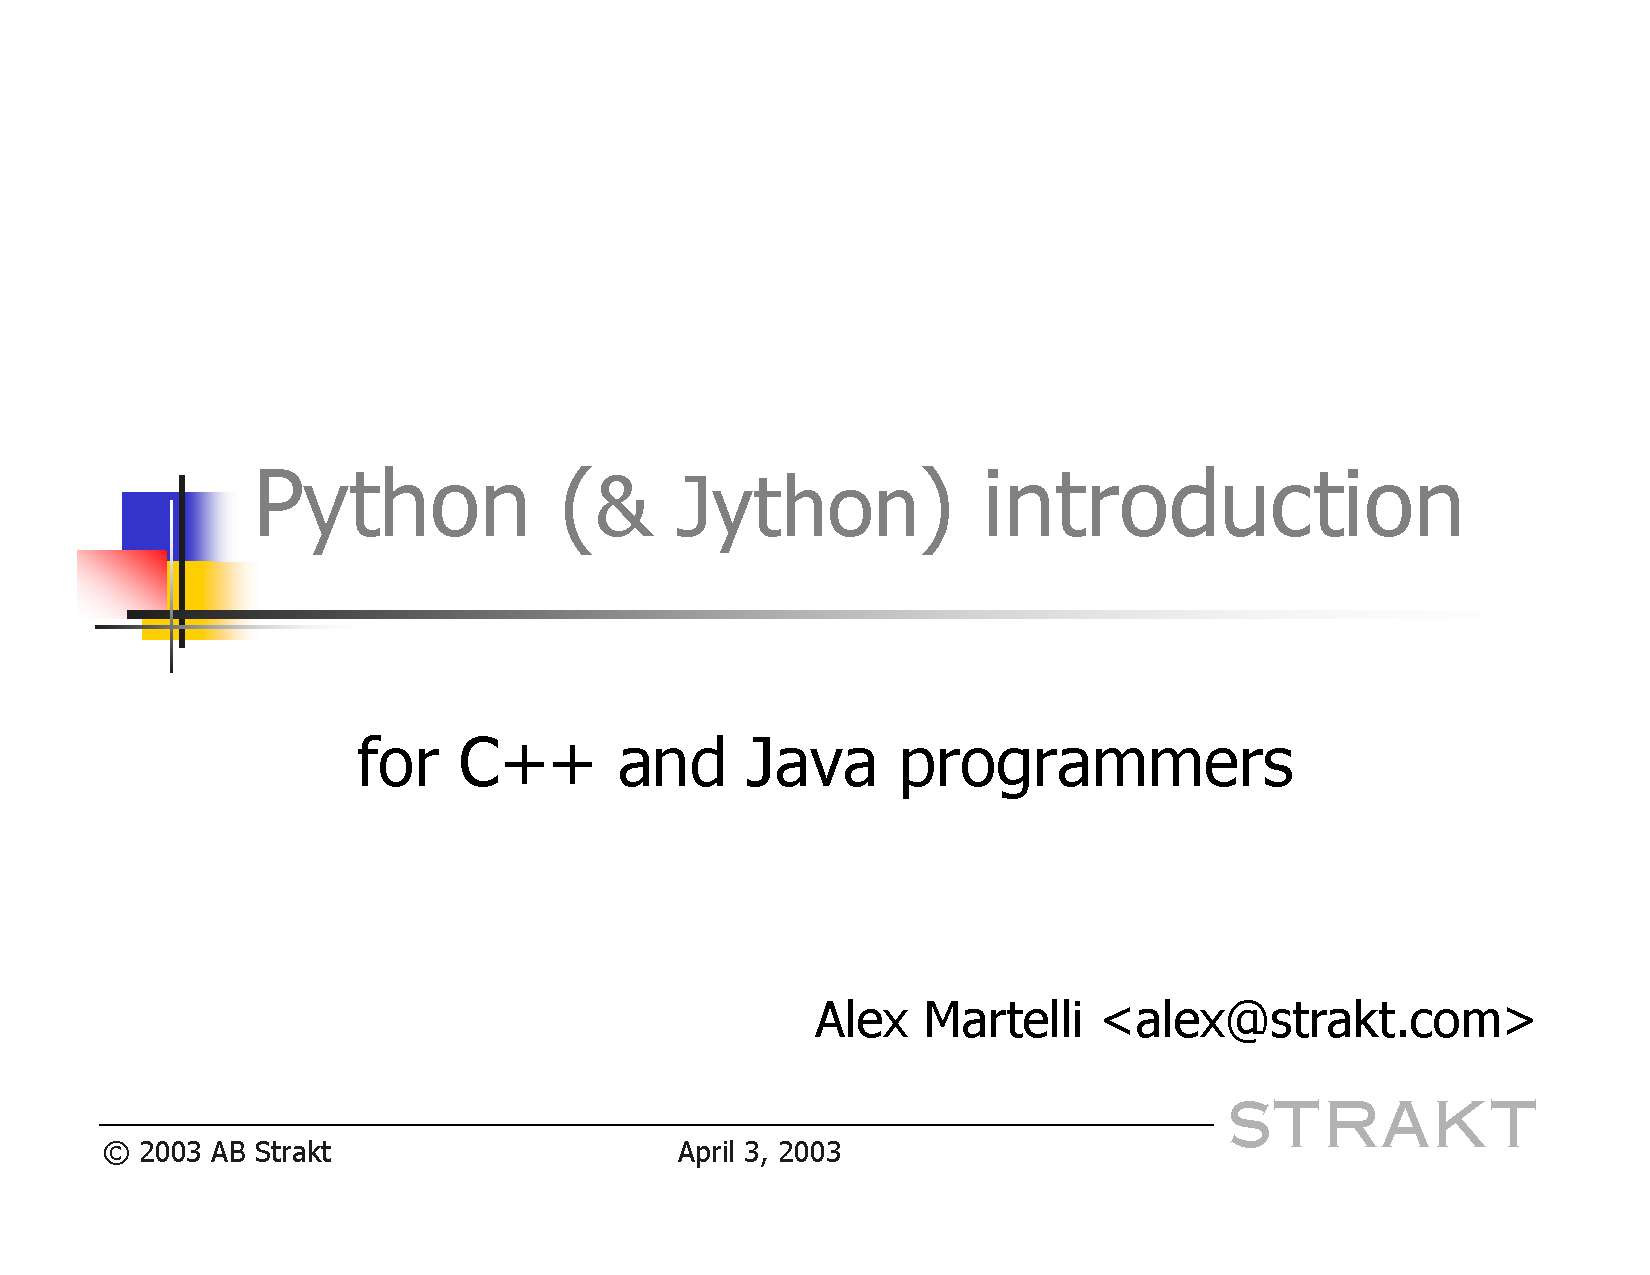
\includepdf[pages={-}]{notes/alex.pdf}

\chapter{Python Tutorial}
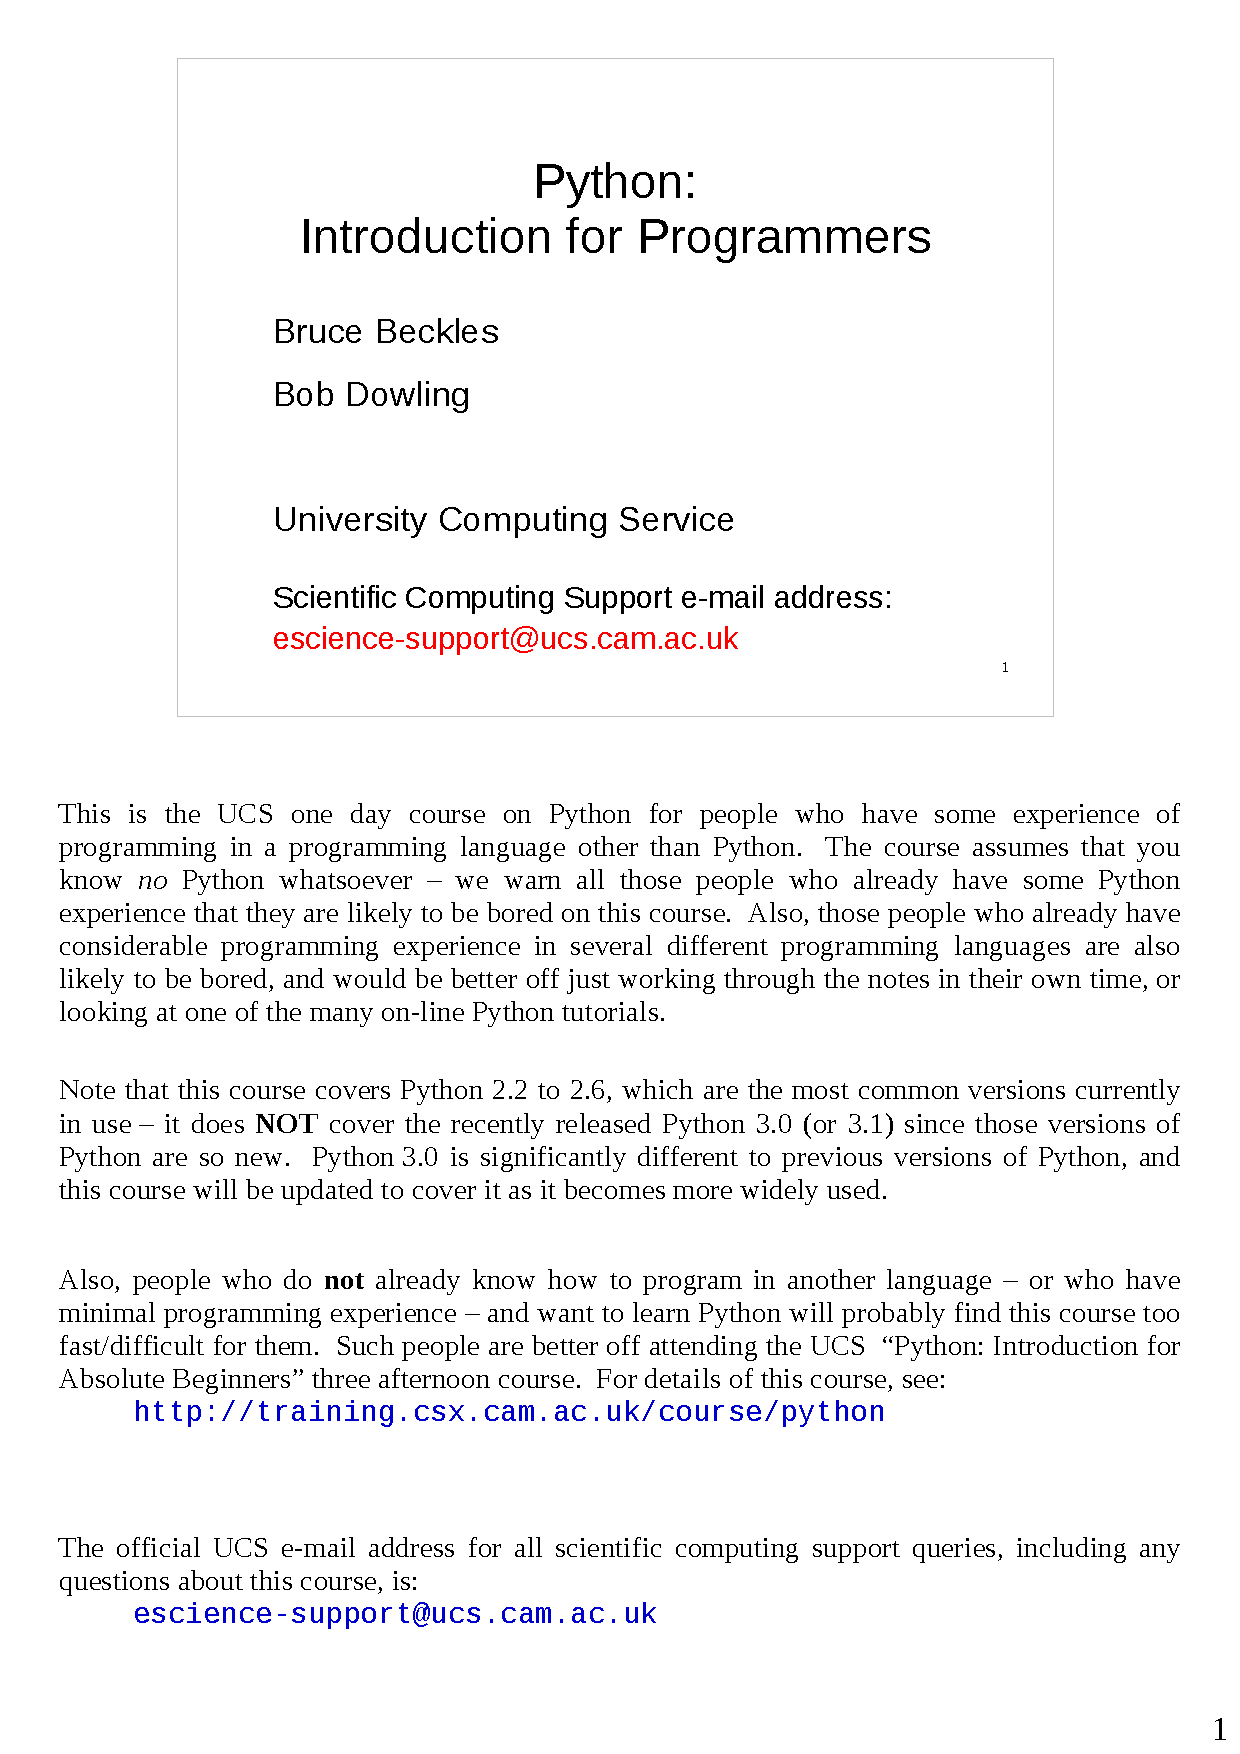
\includepdf[pages={-}]{notes/notes.pdf}

\chapter{Advanced Python}
%will include additions from my ITI Python Slides Tutorial
%Topics to be added include:
% List Comprehension, Functional Programming, etc. 
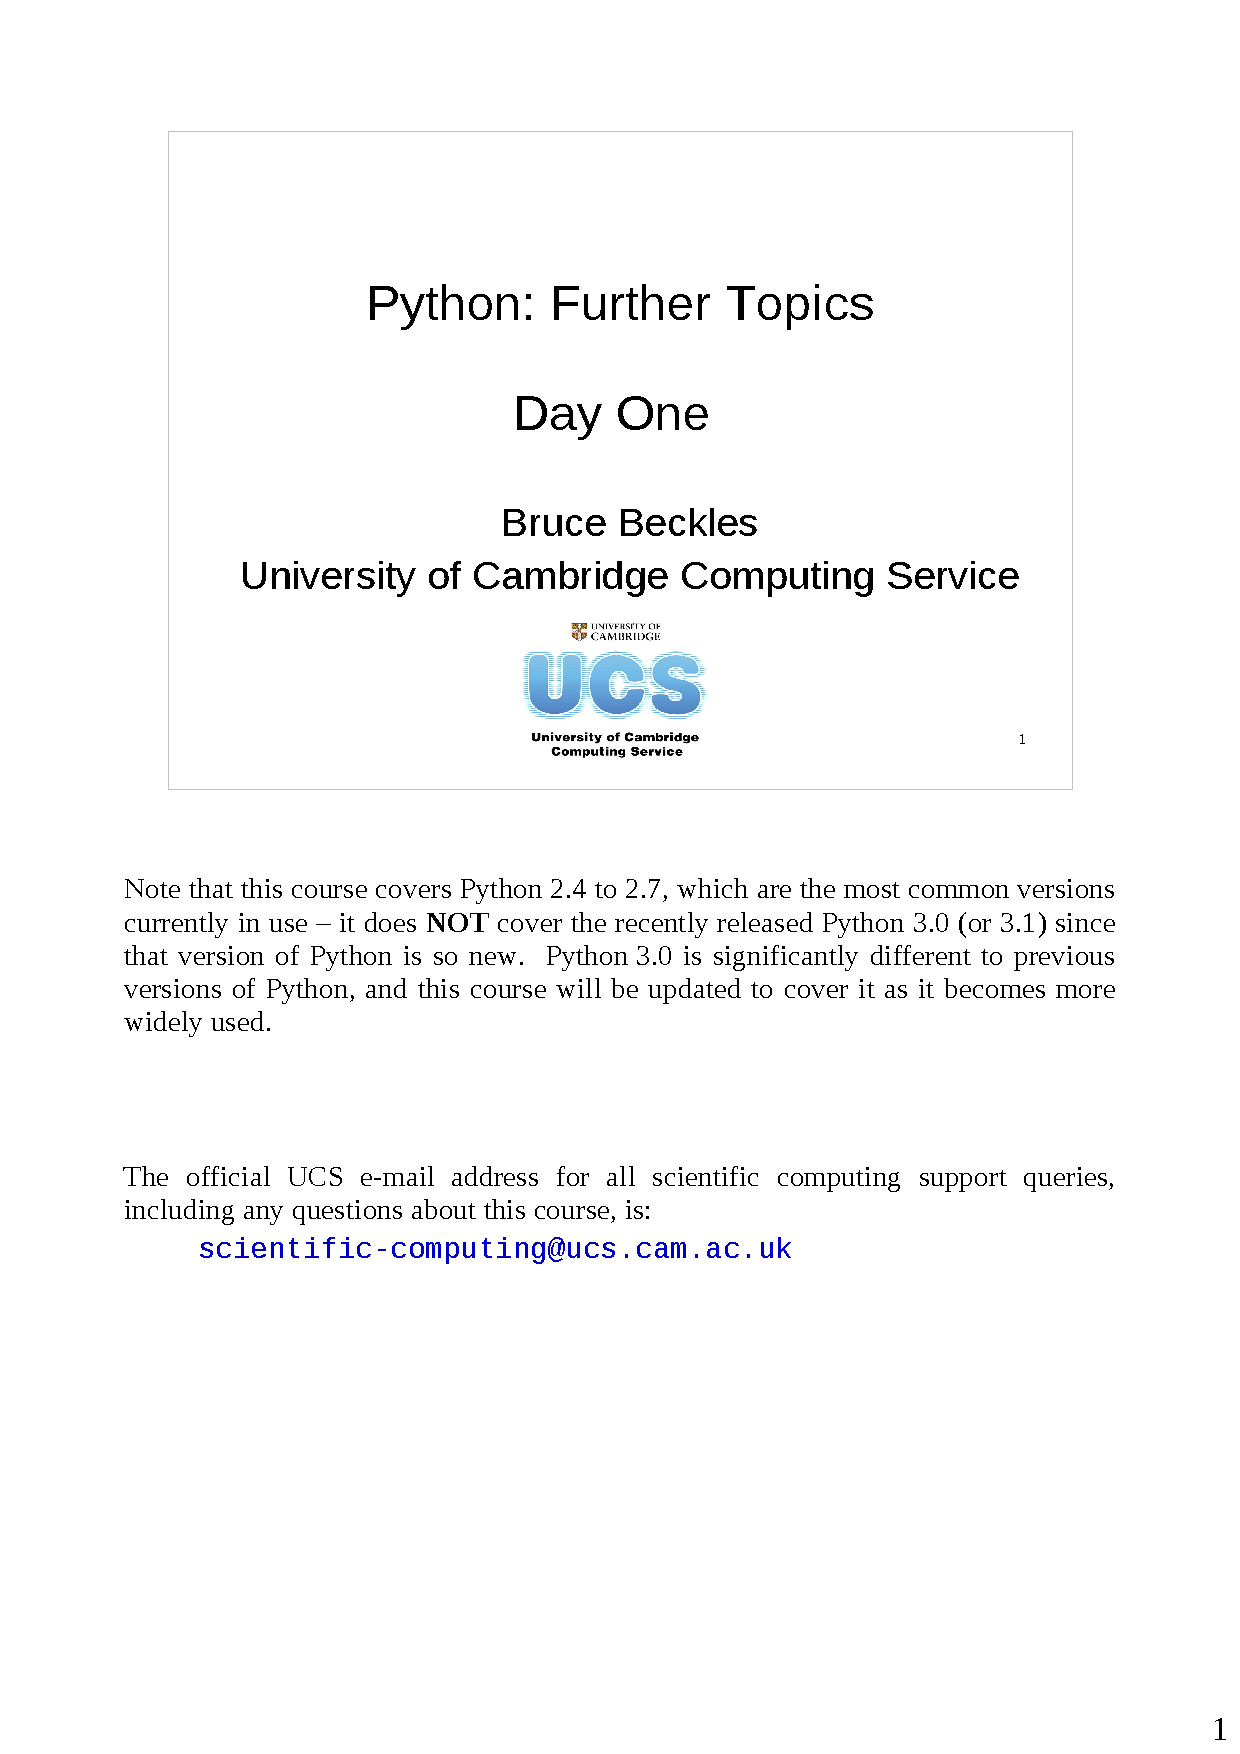
\includepdf[pages={-}]{notes/handout1.pdf}
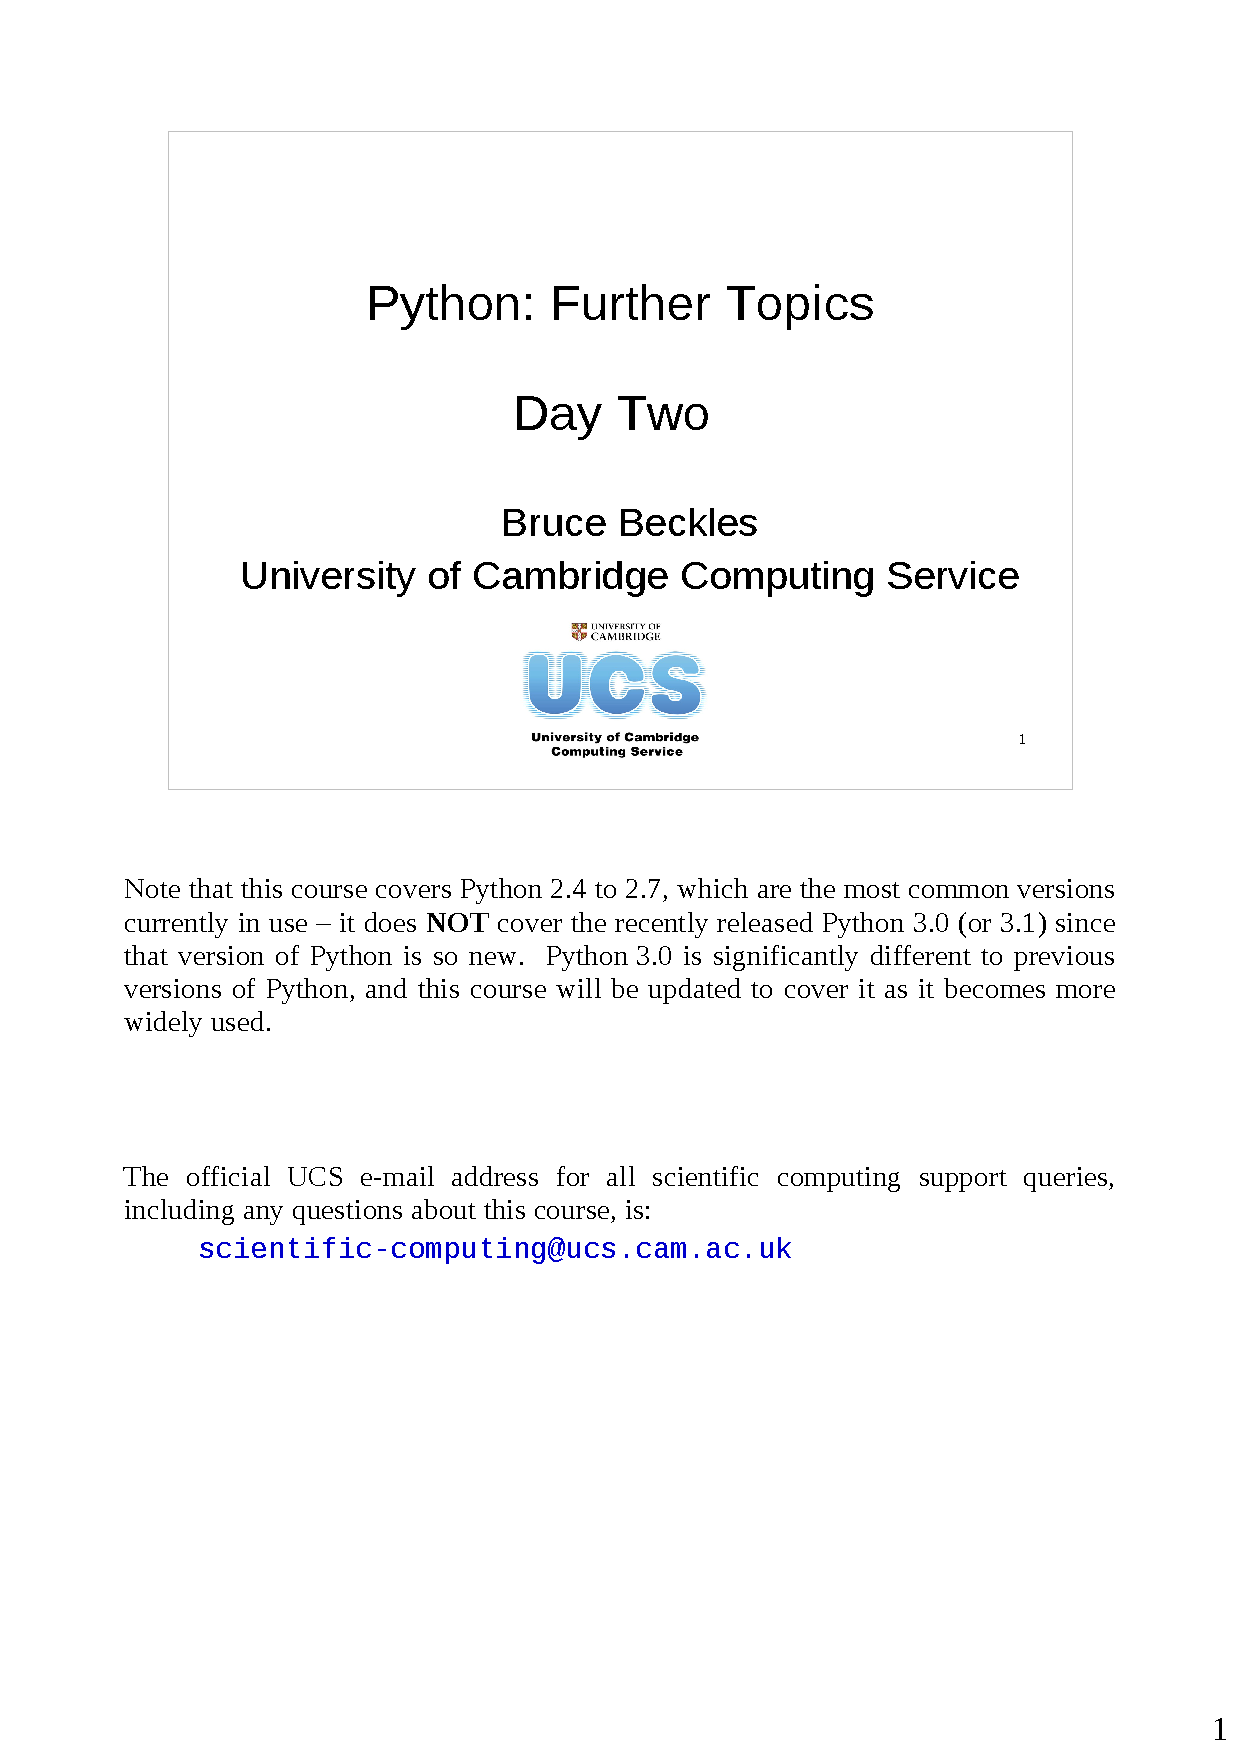
\includepdf[pages={-}]{notes/handout2.pdf}

\chapter{Object Oriented Python Concepts}
\includepdf[pages={166-184}]{notes/project.pdf}

\chapter{Python Magic}
\includepdf[pages={199-231}]{notes/project.pdf}

\chapter{Python GUI}
\includepdf[pages={299-313}]{notes/project.pdf}

\chapter{Network Programming}
\includepdf[pages={326-341}]{notes/project.pdf}

\chapter{Python Facts}
\section{Zip}
Combining lists is really easy using zip.
\begin{lstlisting}
names = ['john', 'peter', 'robert']
ages = [24, 26, 35]
cars = ['BMW', 'Audi', 'Ford']

print zip(names, ages, cars)

>>[('john', 24, 'BMW'), ('peter', 26, 'Audi'), ('robert', 35, 'Ford')]
\end{lstlisting}

\section{List Comprehensions Support Conditions}
You can add conditions to your list comprehensions
\begin{lstlisting}
things = [1,2,'3','dog']
numbers = [t for t in things if t.isdigit()]

>>Traceback (most recent call last):
  File "/base/data/home/apps/s~learnpythonjail/2.365841894475711898/main.py", line 75, in execute_python
    exec(code, {})
  File "<string>", line 2, in <module>
AttributeError: 'int' object has no attribute 'isdigit'
\end{lstlisting}

\section{Expanding arrays to function arguments}
To pass a list of arguments to a function using an array, use the following notation:
\begin{lstlisting}
def add(n1, n2):
    return n1 + n2

numbers = [3, 4]
print add(*numbers)

>>7
\end{lstlisting}

\section{Ordered and Named Function Arguments}
You can accept variable amounts of function parameters by name and by order
\begin{lstlisting}
def f(*args, **kwargs):
    print(args)
    print(kwargs)

f(1,2,3,named1="keyword arg1", another="another kwarg")

>>
(1, 2, 3)
{'named1': 'keyword arg1', 'another': 'another kwarg'}
\end{lstlisting}

\section{Functions as objects}
Everything is an object. Functions are true objects, so they can be passed as arguments
\begin{lstlisting}
def talk(text):
    print text

def think(idea):
    print "thinking about %s" % idea

def do_something(what, with_what):
    what(with_what)

do_something(talk, 'hello!')
do_something(think, 'food...')

>>
hello!
thinking about food...
\end{lstlisting}

\section{Mutability}
identifiers point to objects, so a change to a mutable object (like a list) will change it no matter how it's identified. To make a copy of a list, slice it, or use copy (or deepcopy).
\begin{lstlisting}
original_list = ['a','b','c']
copy_of_original_list = original_list
copy_of_original_list.pop()
print original_list


original_list = ['a','b','c']
copy_of_original_list = original_list[:]  # added 3 characters in this statement
copy_of_original_list.pop()
print original_list

>>
['a', 'b']
['a', 'b', 'c']
\end{lstlisting}

\section{Change mutable lists using another name}
Changing one list can change another list, which can hide bugs or obfuscate code.
\begin{lstlisting}
congratulatory_message = list("Lucky You!")

temp = congratulatory_message
for x in range(0,8,4):
    temp[x] = chr((8-x)*10)

# Looks like I never changed the congratulatory message...
print "".join(congratulatory_message)

>>
Puck( You!
\end{lstlisting}

\section{Factorial Function}
There are probably as many different non-native implementations of the factorial function in Python as there are stars in the sky, but this one shines particularly bright. This lambda function uses reduce to iterate through numbers from 2 to n, multiplying them as it goes along. Note that the third argument to reduce is the default value, which is returned if the sequence given by xrange is empty (e.g. if n is zero or one).
\begin{lstlisting}
from operator import mul
factorial = lambda n: reduce(mul, xrange(2, n+1), 1)
print factorial(21)
>>
51090942171709440000
\end{lstlisting}

\section{String formatting using dictionaries}
Python has really powerful string formatting. If you want to use dictionary based (template-like) formatting, then you can:
\begin{lstlisting}
data = {"name" : "Alfred"}
print "Hello %(name)s! How are you?" % data

>>Output:
Hello Alfred! How are you?
\end{lstlisting}

\section{Never Define One Line Functions}
Lambdas are Python's way of telling you to avoid overusing def. 

\begin{lstlisting}
from math import sqrt
def quad(a, b, c):
    return -b/a + sqrt(b**2-4*a*c), -b/a + sqrt(b**2-4*a*c)
roots = lambda a, b, c: (-b/a + sqrt(b**2-4*a*c), -b/a + sqrt(b**2-4*a*c))
#Use with caution.

>>Output
\end{lstlisting}

\section{Number from Digits}
Turn a list of digits to a number.
\begin{lstlisting}
digit_list = [1,2,3,4,5]
print reduce(lambda x,y: 10*x+y, digit_list)
>>Output:
12345
\end{lstlisting}

\section{Generator Functions}
Python supports generator functions, which create iteratable sequences on the fly:
\begin{lstlisting}
def lottery_numbers():
    my_numbers = [1,3,2,5,4,6]

    for n in my_numbers:
        if n > 3:
            yield n+10
        else:
            yield n

for n in lottery_numbers():
    print n

>>Output:
1
3
2
15
14
16
\end{lstlisting}

\section{Parsing REST API}
Python is really awesome when it comes to API integration. Check out how easy it is to search Twitter:
\begin{lstlisting}
import urllib, simplejson, pprint
data = simplejson.load(urllib.urlopen("http://search.twitter.com/search.json?q=learnpython&count=5"))
pprint.pprint([x["text"] for x in data["results"]])
\end{lstlisting}

\section{Sets for finding unions and intersections}
Using set operations is powerful. Find the elements common to all lists in a list of lists.
\begin{lstlisting}
def get_common_elements(list_of_lists):
    return list(set.intersection(*map(set, list_of_lists)))

a = [1,2,3,4,5,6,7,8,9,10]
b = [2,4,6,8,10,12,14,16,18,20]
print get_common_elements([a,b])
print list(set.union( set(a), set(b) ))

>>Output:
[8, 2, 4, 10, 6]
[1, 2, 3, 4, 5, 6, 7, 8, 9, 10, 12, 14, 16, 18, 20]

\end{lstlisting}


\section{Locals and strings}
Use locals for easy string interpolation.

\begin{lstlisting}
world = "earth"
print "hello %(world)s" % locals()

>>Output:
hello earth

\end{lstlisting}


\section{Encoding \& Decoding}
Python supports a wide variety of encoding and decoding methods.
\begin{lstlisting}
print "ABCDEFGH".encode("hex")
print 'VGhpcyBpcyBhIHNlY3JldCBNZXNzYWdl\n'.decode("base64")

>>Output:
4142434445464748
This is a secret Message
\end{lstlisting}

\section{Set Comprehensions}
Python 2.7 supports set literals and comprehensions.

\begin{lstlisting}
print {1, 2, 2, 3, 1}

names = ["Foo", "bar", "foo", "Baz", "CATS", "dogs"]
print {name.upper() for name in names if name[0] in 'fFbB'}

>>Output:
set([1, 2, 3])
set(['BAZ', 'FOO', 'BAR'])
\end{lstlisting}


\section{dict() and zip() make for a powerful combination}
Create dicts by ziping keys and data.
\begin{lstlisting}
voters = ['friends','neighbors','countrymen']
counts = [10,5,800]
print dict(zip(voters,counts))

votes = ['yes',66,'no',77,'abstain',9]
print dict(zip(votes[:-1:2],votes[1::2]))

>>Output:
{'neighbors': 5, 'countrymen': 800, 'friends': 10}
{'yes': 66, 'abstain': 9, 'no': 77}
\end{lstlisting}

\section{Bools inherit from int}
Check help(True) for more details.
\begin{lstlisting}
print True + True == 2
>>Output:
True
\end{lstlisting}


\section{The Zen of Python}
Long time Pythoneer Tim Peters succinctly channels the BDFL's guiding principles for Python's design into 20 aphorisms, only 19 of which have been written down.
\begin{lstlisting}
import this
\end{lstlisting}

\chapter{Python Glossary}
This is a glossary of terms and topics in Python as covered in Codecademy courses. It does not attempt to completely define and explain terms, but rather provides a general overview that is appropriate for someone new to the language. For a more comprehensive treatment of these topics, we recommend the Mozilla Developer Network Python documentation.

\section{List}
 A Python data type that holds an ordered collection of values, which can be of any type. This is equivalant to an "array" in many other languages. Python lists are "mutable," implying that they can be changed once created.
\lstset{language=Python, tabsize=4}
\begin{lstlisting}
>> x = [1, 2, 3, 4]
>> y = ['spam', 'eggs']
>> x
[1, 2, 3, 4]
>> y
['spam','eggs']

>> y.append('mash')
>> y
['spam', 'eggs', 'mash']

>> y += ['beans']
>> y
['spam', 'eggs', 'mash', 'beans']
\end{lstlisting}

\section{Slice}
A pythonic way of extracting "slices" of a list using a special bracket notation that specifies the start and end of the section of the list you wish to extract. Leaving the beginning value blank indicates you wish to start at the beginning of the list, leaving the ending value blank indicates you wish to go to the end of the list. Using a negative value references the end of the list (so that in a list of 4 elements, -1 means the 4th element). Slicing always yields another list, even when extracting a single value. 
\lstset{language=Python, tabsize=4}
\begin{lstlisting}
>> # Specifying a beginning and end:
>> x = [1, 2, 3, 4]
>> x[2:3]
[3]

>> # Specifying start at the beginning and end at the second element
>> x[:2]
[1, 2]

>> # Specifying start at the next to last element and go to the end
>> x[-2:]
[3, 4]

>> # Specifying start at the beginning and go to the next to last element
>> x[:-1]
[1, 2, 3]

>> # Specifying a step argument returns every n-th item
>> y = [1, 2, 3, 4, 5, 6, 7, 8]
>> y[::2]
[1, 3, 5, 7]

>> # Return a reversed version of the list ( or string )
>> x[::-1]
[4, 3, 2, 1]

>> # String reverse
>> my_string = "Aloha"
>> my_string[::-1]
"aholA"
\end{lstlisting}

\section{Variables}
Variables are assigned values using the '=' operator, which is not to be confused with the '==' sign used for testing equality. A variable can hold almost any type of value such as lists, dictionaries, functions. 
\lstset{language=Python, tabsize=4}
\begin{lstlisting}
>> x = 12
>> x
12
\end{lstlisting}

\section{Functions}
 Python builds functions using the syntax: $def function\_name(variable): $ Functions can be stand-alone or can return values. Functions can also contain other functions.
\lstset{language=Python, tabsize=4}
\begin{lstlisting}
def add_two(a, b):
  c = a + b
  return c

# or without the interim assignment to c
def add_two(a, b):
  return a + b
\end{lstlisting}

\section{Tuples}
A Python data type that holds an ordered collection of values, which can be of any type. Python tuples are "immutable," meaning that they cannot be changed once created. 
\lstset{language=Python, tabsize=4}
\begin{lstlisting}
>> x = (1, 2, 3, 4)
>> y = ('spam', 'eggs')

>> my_list = [1,2,3,4]
>> my_tuple = tuple(my_list)
>> my_tuple
(1, 2, 3, 4)
\end{lstlisting}


\section{List Comprehensions}

Convenient ways to generate or extract information from lists. List Comprehensions will take a general form such as: [item for item in List if Condition]

\lstset{language=Python, tabsize=4}
\begin{lstlisting}
>> x_list = [1,2,3,4,5,6,7]
>> even_list = [num for num in x_list if (num % 2 == 0)]
>> even_list
[2,4,6]

>> m_list = ['AB', 'AC', 'DA', 'FG', 'LB']
>> A_list = [duo for duo in m_list if ('A' in duo)]
>> A_list
['AB', 'AC', 'DA']
\end{lstlisting}

\section{Sets}

Sets are collections of unique but unordered items. It is possible to convert certain iterables to a set. {"this", "is", "a", "set"}

\lstset{language=Python, tabsize=4}
\begin{lstlisting}

>> new_set = {1, 2, 3, 4, 4, 4,'A', 'B', 'B', 'C'}
>> new_set
{'A', 1, 'C', 3, 4, 2, 'B'}

>> dup_list = [1,1,2,2,2,3,4,55,5,5,6,7,8,8]
>> set_from_list = set(dup_list)
>> set_from_list
{1, 2, 3, 4, 5, 6, 7, 8, 55}
\end{lstlisting}

\section{Dictionaries}

Dictionaries, like sets, contain unique but unordered items. The big difference is the concept of "keys" to retrieve "values"; "keys" can be strings, integers or tuples (or anything else hashable), but the "values" that they map to can be any data type.

\lstset{language=Python, tabsize=4}
\begin{lstlisting}
>> my_dict = {}
>> content_of_value1 = "abcd"
>> content_of_value2 = "wxyz"
>> my_dict.update({"key_name1":content_of_value1})
>> my_dict.update({"key_name2":content_of_value2})
>> my_dict
{'key_name1':"abcd", 'key_name2':"wxyz"}
>> my_dict.get("key_name2")
"wxyz"
\end{lstlisting}

\section{Strings}

Strings store characters and have many built-in convenience methods that let you modify their content.

\lstset{language=Python, tabsize=4}
\begin{lstlisting}
>> my_string1 = "this is a valid string"
>> my_string2 = 'this is also a valid string'
>> my_string3 = 'this is' + ' ' + 'also' + ' ' + 'a string'
>> my_string3
"this is also a string"
\end{lstlisting}

\section{The len() Function}

Using $len(some\_object)$ returns the number of $\_top\-level\_$ items contained in the object being queried.

\lstset{language=Python, tabsize=4}
\begin{lstlisting}

>> my_list = [0,4,5,2,3,4,5]
>> len(my_list)
7

>> my_string = 'abcdef'
>> len(my_string)
6
\end{lstlisting}


\section{Single Line Comments}

Augmenting code with human readable descriptions can help document design decisions.

\begin{lstlisting}
# this is a single line comment.
\end{lstlisting}

\section{Multi-line Comments}

Some comments need to span several lines, use this if you have more than 4 single line comments in a row.
\begin{lstlisting}

'''
this is
a multi-line
comment, i am handy for commenting out whole
chunks of code very fast
'''
\end{lstlisting}

\section{Print}

A function to display the output of a program. Using the parenthesized version is arguably more consistent.

\begin{lstlisting}
>> # this will work in all modern versions of Python
>> print("some text here")
"some text here"

>> # but this only works in Python versions lower than 3.x
>> print "some text here too"
"some text here too"
\end{lstlisting}

\section{The range() Function}

The range() function returns a list of integers, the sequence of which is defined by the arguments passed to it.

argument variations:
\begin{itemize}
\item range(terminal)
\item range(start, terminal)
\item range(start, terminal, step\_size)
\end{itemize}

\begin{lstlisting}
>> [i for i in range(4)]
[0, 1, 2, 3]

>> [i for i in range(2, 8)]
[2, 3, 4, 5, 6, 7]

>> [i for i in range(2, 13, 3)]
[2, 5, 8, 11]
\end{lstlisting}

\section{For Loops}

Python provides a clean iteration syntax. Note the colon and indentation.

\begin{lstlisting}
>> for i in range(0, 3):
>>     print(i*2)
0
2
4

>> m_list = ["Sir", "Lancelot", "Coconuts"]
>> for item in m_list:
>>     print(item)
Sir
Lancelot
Coconuts

>> w_string = "Swift"
>> for letter in w_string:
>>     print(letter)
S
w
i
f
t
\end{lstlisting}

\section{While Loops}

A While loop permits code to execute repeatedly until a certain condition is met. This is useful if the number of iterations required to complete a task is unknown prior to flow entering the loop.

\begin{lstlisting}
>> looping_needed = True
>>
>> while looping_needed:
>>     # some operation on data
>>     if condition:
>>          looping_needed = False
\end{lstlisting}

\section{The str() Function}

Using the str() function allows you to represent the content of a variable as a string, provided that the data type of the variable provides a neat way to do so. str() does not change the variable in place, it returns a 'stringified' version of it.

\begin{lstlisting}
>> # such features can be useful for concatenating strings
>> my_var = 123
>> my_var
123

>> str(my_var)
'123'

>> my_booking = "DB Airlines Flight " + str(my_var)
>> my_booking
'DB Airlines Flight 123'
\end{lstlisting}

\section{>>>}
The default Python prompt of the interactive shell. Often seen for code examples which can be executed interactively in the interpreter.

\section{...}
The default Python prompt of the interactive shell when entering code for an indented code block or within a pair of matching left and right delimiters (parentheses, square brackets or curly braces).

\section{2to3}
A tool that tries to convert Python 2.x code to Python 3.x code by handling most of the incompatibilities which can be detected by parsing the source and traversing the parse tree.

2to3 is available in the standard library as lib2to3; a standalone entry point is provided as Tools/scripts/2to3. See 2to3 - Automated Python 2 to 3 code translation.

\section{abstract base class}
Abstract base classes complement duck-typing by providing a way to define interfaces when other techniques like hasattr() would be clumsy or subtly wrong (for example with magic methods). ABCs introduce virtual subclasses, which are classes that don’t inherit from a class but are still recognized by isinstance() and issubclass(); see the abc module documentation. Python comes with many built-in ABCs for data structures (in the collections module), numbers (in the numbers module), and streams (in the io module). You can create your own ABCs with the abc module.

\section{argument}
A value passed to a function (or method) when calling the function. There are two types of arguments:
\begin{itemize}
\item keyword argument: an argument preceded by an identifier (e.g. name=) in a function call or passed as a value in a dictionary preceded by **. For example, 3 and 5 are both keyword arguments in the following calls to complex():
\begin{lstlisting}
complex(real=3, imag=5)
complex(**{'real': 3, 'imag': 5})
\end{lstlisting}
\item positional argument: an argument that is not a keyword argument. Positional arguments can appear at the beginning of an argument list and/or be passed as elements of an iterable preceded by *. For example, 3 and 5 are both positional arguments in the following calls:
\begin{lstlisting}
complex(3, 5)
complex(*(3, 5))
\end{lstlisting}
\end{itemize}
Arguments are assigned to the named local variables in a function body. See the Calls section for the rules governing this assignment. Syntactically, any expression can be used to represent an argument; the evaluated value is assigned to the local variable.

\section{attribute}
A value associated with an object which is referenced by name using dotted expressions. For example, if an object o has an attribute a it would be referenced as o.a.

\section{BDFL}
Benevolent Dictator For Life, a.k.a. Guido van Rossum, Python’s creator.

\section{bytecode}
Python source code is compiled into bytecode, the internal representation of a Python program in the CPython interpreter. The bytecode is also cached in .pyc and .pyo files so that executing the same file is faster the second time (recompilation from source to bytecode can be avoided). This “intermediate language” is said to run on a virtual machine that executes the machine code corresponding to each bytecode. Do note that bytecodes are not expected to work between different Python virtual machines, nor to be stable between Python releases.

A list of bytecode instructions can be found in the documentation for the dis module.

\section{class}
A template for creating user-defined objects. Class definitions normally contain method definitions which operate on instances of the class.

\section{classic class}
Any class which does not inherit from object. See new-style class. Classic classes have been removed in Python 3.

\section{coercion}
The implicit conversion of an instance of one type to another during an operation which involves two arguments of the same type. For example, int(3.15) converts the floating point number to the integer 3, but in 3+4.5, each argument is of a different type (one int, one float), and both must be converted to the same type before they can be added or it will raise a TypeError. Coercion between two operands can be performed with the coerce built-in function; thus, 3+4.5 is equivalent to calling operator.add(*coerce(3, 4.5)) and results in operator.add(3.0, 4.5). Without coercion, all arguments of even compatible types would have to be normalized to the same value by the programmer, e.g., float(3)+4.5 rather than just 3+4.5.

\section{complex number}
An extension of the familiar real number system in which all numbers are expressed as a sum of a real part and an imaginary part. Imaginary numbers are real multiples of the imaginary unit (the square root of -1), often written i in mathematics or j in engineering. Python has built-in support for complex numbers, which are written with this latter notation; the imaginary part is written with a j suffix, e.g., 3+1j. To get access to complex equivalents of the math module, use cmath. Use of complex numbers is a fairly advanced mathematical feature. If you’re not aware of a need for them, it’s almost certain you can safely ignore them.

\section{context manager}
An object which controls the environment seen in a with statement. See PEP 343.

\section{CPython}
The canonical implementation of the Python programming language, as distributed on python.org. The term “CPython” is used when necessary to distinguish this implementation from others such as Jython or IronPython.

\section{decorator}
A function returning another function, usually applied as a function transformation using the @wrapper syntax. Common examples for decorators are classmethod() and staticmethod().

The decorator syntax is merely syntactic sugar, the following two function definitions are semantically equivalent:
\begin{lstlisting}
def f(...):
    ...
f = staticmethod(f)

@staticmethod
def f(...):
    ...
\end{lstlisting}

The same concept exists for classes, but is less commonly used there. See the documentation for function definitions and class definitions for more about decorators.

\section{descriptor}
Any new-style object which defines the methods $\_\_$get$\_\_$(), $\_\_$set$\_\_$(), or $\_\_$delete$\_\_$(). When a class attribute is a descriptor, its special binding behavior is triggered upon attribute lookup. Normally, using a.b to get, set or delete an attribute looks up the object named b in the class dictionary for a, but if b is a descriptor, the respective descriptor method gets called. Understanding descriptors is a key to a deep understanding of Python because they are the basis for many features including functions, methods, properties, class methods, static methods, and reference to super classes.

For more information about descriptors’ methods, see Implementing Descriptors.

\section{dictionary}
An associative array, where arbitrary keys are mapped to values.

\section{docstring}
A string literal which appears as the first expression in a class, function or module. While ignored when the suite is executed, it is recognized by the compiler and put into the $\_\_$doc$\_\_$ attribute of the enclosing class, function or module. Since it is available via introspection, it is the canonical place for documentation of the object.

\section{duck-typing}
A programming style which does not look at an object’s type to determine if it has the right interface; instead, the method or attribute is simply called or used (“If it looks like a duck and quacks like a duck, it must be a duck.”) By emphasizing interfaces rather than specific types, well-designed code improves its flexibility by allowing polymorphic substitution. Duck-typing avoids tests using type() or isinstance(). (Note, however, that duck-typing can be complemented with abstract base classes.) Instead, it typically employs hasattr() tests or EAFP programming.

\section{EAFP}
Easier to ask for forgiveness than permission. This common Python coding style assumes the existence of valid keys or attributes and catches exceptions if the assumption proves false. This clean and fast style is characterized by the presence of many try and except statements. The technique contrasts with the LBYL style common to many other languages such as C.

\section{expression}
A piece of syntax which can be evaluated to some value. In other words, an expression is an accumulation of expression elements like literals, names, attribute access, operators or function calls which all return a value. In contrast to many other languages, not all language constructs are expressions. There are also statements which cannot be used as expressions, such as print or if. Assignments are also statements, not expressions.

\section{extension module}
A module written in C or C++, using Python’s C API to interact with the core and with user code.

\section{file object}
An object exposing a file-oriented API (with methods such as read() or write()) to an underlying resource. Depending on the way it was created, a file object can mediate access to a real on-disk file or to another type of storage or communication device (for example standard input/output, in-memory buffers, sockets, pipes, etc.). File objects are also called file-like objects or streams.

There are actually three categories of file objects: raw binary files, buffered binary files and text files. Their interfaces are defined in the io module. The canonical way to create a file object is by using the open() function.

\section{file-like object}
A synonym for file object.

\section{finder}
An object that tries to find the loader for a module. It must implement a method named find\_module(). See PEP 302 for details.

\section{floor division}
Mathematical division that rounds down to nearest integer. The floor division operator is //. For example, the expression 11 // 4 evaluates to 2 in contrast to the 2.75 returned by float true division. Note that (-11) // 4 is -3 because that is -2.75 rounded downward. See PEP 238.

\section{function}
A series of statements which returns some value to a caller. It can also be passed zero or more arguments which may be used in the execution of the body. See also parameter, method, and the Function definitions section.

\section{$\_\_$future$\_\_$}
A pseudo-module which programmers can use to enable new language features which are not compatible with the current interpreter. For example, the expression 11/4 currently evaluates to 2. If the module in which it is executed had enabled true division by executing:

\begin{lstlisting}
from __future__ import division
\end{lstlisting}
the expression 11/4 would evaluate to 2.75. By importing the$\_\_$future$\_\_$ module and evaluating its variables, you can see when a new feature was first added to the language and when it will become the default:
\begin{lstlisting}
>>>
>>> import __future__
>>> __future__.division
_Feature((2, 2, 0, 'alpha', 2), (3, 0, 0, 'alpha', 0), 8192)
\end{lstlisting}

\section{garbage collection}
The process of freeing memory when it is not used anymore. Python performs garbage collection via reference counting and a cyclic garbage collector that is able to detect and break reference cycles.

\section{generator}
A function which returns an iterator. It looks like a normal function except that it contains yield statements for producing a series a values usable in a for-loop or that can be retrieved one at a time with the next() function. Each yield temporarily suspends processing, remembering the location execution state (including local variables and pending try-statements). When the generator resumes, it picks-up where it left-off (in contrast to functions which start fresh on every invocation).

\section{generator expression}
An expression that returns an iterator. It looks like a normal expression followed by a for expression defining a loop variable, range, and an optional if expression. The combined expression generates values for an enclosing function:
\begin{lstlisting}
>>>
>>> sum(i*i for i in range(10))         # sum of squares 0, 1, 4, ... 81
285
\end{lstlisting}

\section{GIL}
See global interpreter lock.

\section{global interpreter lock}
The mechanism used by the CPython interpreter to assure that only one thread executes Python bytecode at a time. This simplifies the CPython implementation by making the object model (including critical built-in types such as dict) implicitly safe against concurrent access. Locking the entire interpreter makes it easier for the interpreter to be multi-threaded, at the expense of much of the parallelism afforded by multi-processor machines.

However, some extension modules, either standard or third-party, are designed so as to release the GIL when doing computationally-intensive tasks such as compression or hashing. Also, the GIL is always released when doing I/O.

Past efforts to create a “free-threaded” interpreter (one which locks shared data at a much finer granularity) have not been successful because performance suffered in the common single-processor case. It is believed that overcoming this performance issue would make the implementation much more complicated and therefore costlier to maintain.

\section{hashable}
An object is hashable if it has a hash value which never changes during its lifetime (it needs a $\_\_$hash$\_\_$() method), and can be compared to other objects (it needs an $\_\_$eq$\_\_$() or $\_\_$cmp$\_\_$() method). Hashable objects which compare equal must have the same hash value.

Hashability makes an object usable as a dictionary key and a set member, because these data structures use the hash value internally.

All of Python’s immutable built-in objects are hashable, while no mutable containers (such as lists or dictionaries) are. Objects which are instances of user-defined classes are hashable by default; they all compare unequal (except with themselves), and their hash value is their id().

\section{IDLE}
An Integrated Development Environment for Python. IDLE is a basic editor and interpreter environment which ships with the standard distribution of Python.

\section{immutable}
An object with a fixed value. Immutable objects include numbers, strings and tuples. Such an object cannot be altered. A new object has to be created if a different value has to be stored. They play an important role in places where a constant hash value is needed, for example as a key in a dictionary.

\section{integer division}
Mathematical division discarding any remainder. For example, the expression 11/4 currently evaluates to 2 in contrast to the 2.75 returned by float division. Also called floor division. When dividing two integers the outcome will always be another integer (having the floor function applied to it). However, if one of the operands is another numeric type (such as a float), the result will be coerced (see coercion) to a common type. For example, an integer divided by a float will result in a float value, possibly with a decimal fraction. Integer division can be forced by using the // operator instead of the / operator. See also $\_\_$future$\_\_$.
\section{importer}
An object that both finds and loads a module; both a finder and loader object.
\section{interactive}
Python has an interactive interpreter which means you can enter statements and expressions at the interpreter prompt, immediately execute them and see their results. Just launch python with no arguments (possibly by selecting it from your computer’s main menu). It is a very powerful way to test out new ideas or inspect modules and packages (remember help(x)).
\section{interpreted}
Python is an interpreted language, as opposed to a compiled one, though the distinction can be blurry because of the presence of the bytecode compiler. This means that source files can be run directly without explicitly creating an executable which is then run. Interpreted languages typically have a shorter development/debug cycle than compiled ones, though their programs generally also run more slowly. See also interactive.
\section{iterable}
An object capable of returning its members one at a time. Examples of iterables include all sequence types (such as list, str, and tuple) and some non-sequence types like dict and file and objects of any classes you define with an $\_\_$iter$\_\_$() or $\_\_$getitem$\_\_$() method. Iterables can be used in a for loop and in many other places where a sequence is needed (zip(), map(), ...). When an iterable object is passed as an argument to the built-in function iter(), it returns an iterator for the object. This iterator is good for one pass over the set of values. When using iterables, it is usually not necessary to call iter() or deal with iterator objects yourself. The for statement does that automatically for you, creating a temporary unnamed variable to hold the iterator for the duration of the loop. See also iterator, sequence, and generator.
\section{iterator}
An object representing a stream of data. Repeated calls to the iterator’s next() method return successive items in the stream. When no more data are available a StopIteration exception is raised instead. At this point, the iterator object is exhausted and any further calls to its next() method just raise StopIteration again. Iterators are required to have an $\_\_$iter$\_\_$() method that returns the iterator object itself so every iterator is also iterable and may be used in most places where other iterables are accepted. One notable exception is code which attempts multiple iteration passes. A container object (such as a list) produces a fresh new iterator each time you pass it to the iter() function or use it in a for loop. Attempting this with an iterator will just return the same exhausted iterator object used in the previous iteration pass, making it appear like an empty container.

More information can be found in Iterator Types.

\section{key function}
A key function or collation function is a callable that returns a value used for sorting or ordering. For example, locale.strxfrm() is used to produce a sort key that is aware of locale specific sort conventions.

A number of tools in Python accept key functions to control how elements are ordered or grouped. They include min(), max(), sorted(), list.sort(), heapq.nsmallest(), heapq.nlargest(), and itertools.groupby().

There are several ways to create a key function. For example. the str.lower() method can serve as a key function for case insensitive sorts. Alternatively, an ad-hoc key function can be built from a lambda expression such as lambda r: (r[0], r[2]). Also, the operator module provides three key function constructors: attrgetter(), itemgetter(), and methodcaller(). See the Sorting HOW TO for examples of how to create and use key functions.

\section{keyword argument}
See argument.

\section{lambda}
An anonymous inline function consisting of a single expression which is evaluated when the function is called. The syntax to create a lambda function is lambda [arguments]: expression
\section{LBYL}
Look before you leap. This coding style explicitly tests for pre-conditions before making calls or lookups. This style contrasts with the EAFP approach and is characterized by the presence of many if statements.

In a multi-threaded environment, the LBYL approach can risk introducing a race condition between “the looking” and “the leaping”. For example, the code, if key in mapping: return mapping[key] can fail if another thread removes key from mapping after the test, but before the lookup. This issue can be solved with locks or by using the EAFP approach.

\section{list}
A built-in Python sequence. Despite its name it is more akin to an array in other languages than to a linked list since access to elements are O(1).

\section{list comprehension}
A compact way to process all or part of the elements in a sequence and return a list with the results. result = $["0x\%02x" \% x for x in range(256) if x \% 2 == 0]$ generates a list of strings containing even hex numbers (0x..) in the range from 0 to 255. The if clause is optional. If omitted, all elements in range(256) are processed.

\section{loader}
An object that loads a module. It must define a method named load\_module(). A loader is typically returned by a finder. See PEP 302 for details.

\section{mapping}
A container object that supports arbitrary key lookups and implements the methods specified in the Mapping or MutableMapping abstract base classes. Examples include dict, collections.defaultdict, collections.OrderedDict and collections.Counter.

\section{metaclass}
The class of a class. Class definitions create a class name, a class dictionary, and a list of base classes. The metaclass is responsible for taking those three arguments and creating the class. Most object oriented programming languages provide a default implementation. What makes Python special is that it is possible to create custom metaclasses. Most users never need this tool, but when the need arises, metaclasses can provide powerful, elegant solutions. They have been used for logging attribute access, adding thread-safety, tracking object creation, implementing singletons, and many other tasks.

More information can be found in Customizing class creation.

\section{method}
A function which is defined inside a class body. If called as an attribute of an instance of that class, the method will get the instance object as its first argument (which is usually called self). See function and nested scope.

\section{method resolution order}
Method Resolution Order is the order in which base classes are searched for a member during lookup. See The Python 2.3 Method Resolution Order.

\section{MRO}
See method resolution order.

\section{mutable}
Mutable objects can change their value but keep their id(). See also immutable.

\section{named tuple}
Any tuple\-like class whose indexable elements are also accessible using named attributes (for example, time.localtime() returns a tuple\-like object where the year is accessible either with an index such as t[0] or with a named attribute like t.tm\_year).

A named tuple can be a built-in type such as time.struct\_time, or it can be created with a regular class definition. A full featured named tuple can also be created with the factory function collections.namedtuple(). The latter approach automatically provides extra features such as a self-documenting representation like Employee(name='jones', title='programmer').

\section{namespace}
The place where a variable is stored. Namespaces are implemented as dictionaries. There are the local, global and built-in namespaces as well as nested namespaces in objects (in methods). Namespaces support modularity by preventing naming conflicts. For instance, the functions $\_\_$builtin$\_\_$.open() and os.open() are distinguished by their namespaces. Namespaces also aid readability and maintainability by making it clear which module implements a function. For instance, writing random.seed() or itertools.izip() makes it clear that those functions are implemented by the random and itertools modules, respectively.

\section{nested scope}
The ability to refer to a variable in an enclosing definition. For instance, a function defined inside another function can refer to variables in the outer function. Note that nested scopes work only for reference and not for assignment which will always write to the innermost scope. In contrast, local variables both read and write in the innermost scope. Likewise, global variables read and write to the global namespace.

\section{new-style class}
Any class which inherits from object. This includes all built-in types like list and dict. Only new-style classes can use Python’s newer, versatile features like $\_\_$slots$\_\_$, descriptors, properties, and $\_\_$getattribute$\_\_$().

More information can be found in New-style and classic classes.

\section{object}
Any data with state (attributes or value) and defined behavior (methods). Also the ultimate base class of any new-style class.

\section{parameter}
A named entity in a function (or method) definition that specifies an argument (or in some cases, arguments) that the function can accept. There are four types of parameters:
\begin{itemize}
\item positional-or-keyword: specifies an argument that can be passed either positionally or as a keyword argument. This is the default kind of parameter, for example foo and bar in the following:
\begin{lstlisting}
def func(foo, bar=None): ...
\end{lstlisting}
\item positional-only: specifies an argument that can be supplied only by position. Python has no syntax for defining positional-only parameters. However, some built-in functions have positional-only parameters (e.g. abs()).

\item var-positional: specifies that an arbitrary sequence of positional arguments can be provided (in addition to any positional arguments already accepted by other parameters). Such a parameter can be defined by prepending the parameter name with *, for example args in the following:
\begin{lstlisting}
def func(*args, **kwargs): ...
\end{lstlisting}
\item var-keyword: specifies that arbitrarily many keyword arguments can be provided (in addition to any keyword arguments already accepted by other parameters). Such a parameter can be defined by prepending the parameter name with **, for example kwargs in the example above.
\end{itemize}

Parameters can specify both optional and required arguments, as well as default values for some optional arguments.

See also the argument glossary entry, the FAQ question on the difference between arguments and parameters, and the Function definitions section.

\section{positional argument}
See argument.

\section{Python 3000}
Nickname for the Python 3.x release line (coined long ago when the release of version 3 was something in the distant future.) This is also abbreviated “Py3k”.

\section{Pythonic}
An idea or piece of code which closely follows the most common idioms of the Python language, rather than implementing code using concepts common to other languages. For example, a common idiom in Python is to loop over all elements of an iterable using a for statement. Many other languages don’t have this type of construct, so people unfamiliar with Python sometimes use a numerical counter instead:
\begin{lstlisting}
for i in range(len(food)):
    print food[i]
\end{lstlisting}
As opposed to the cleaner, Pythonic method:
\begin{lstlisting}
for piece in food:
    print piece
reference count
\end{lstlisting}
The number of references to an object. When the reference count of an object drops to zero, it is deallocated. Reference counting is generally not visible to Python code, but it is a key element of the CPython implementation. The sys module defines a getrefcount() function that programmers can call to return the reference count for a particular object.
\section{$\_\_$slots$\_\_$}
A declaration inside a new-style class that saves memory by pre-declaring space for instance attributes and eliminating instance dictionaries. Though popular, the technique is somewhat tricky to get right and is best reserved for rare cases where there are large numbers of instances in a memory-critical application.
\section{sequence}
An iterable which supports efficient element access using integer indices via the $\_\_$getitem$\_\_$() special method and defines a len() method that returns the length of the sequence. Some built-in sequence types are list, str, tuple, and unicode. Note that dict also supports $\_\_$getitem$\_\_$() and $\_\_$len$\_\_$(), but is considered a mapping rather than a sequence because the lookups use arbitrary immutable keys rather than integers.
\section{slice}
An object usually containing a portion of a sequence. A slice is created using the subscript notation, [] with colons between numbers when several are given, such as in variable\_name[1:3:5]. The bracket (subscript) notation uses slice objects internally (or in older versions, $\_\_$getslice$\_\_$() and $\_\_$setslice$\_\_$()).
\section{special method}
A method that is called implicitly by Python to execute a certain operation on a type, such as addition. Such methods have names starting and ending with double underscores. Special methods are documented in Special method names.
\section{statement}
A statement is part of a suite (a “block” of code). A statement is either an expression or a one of several constructs with a keyword, such as if, while or for.
\section{struct sequence}
A tuple with named elements. Struct sequences expose an interface similiar to named tuple in that elements can either be accessed either by index or as an attribute. However, they do not have any of the named tuple methods like \_make() or \_asdict(). Examples of struct sequences include sys.float\_info and the return value of os.stat().

\section{type}
The type of a Python object determines what kind of object it is; every object has a type. An object’s type is accessible as its $\_\_$class$\_\_$ attribute or can be retrieved with type(obj).

\section{view}
The objects returned from dict.viewkeys(), dict.viewvalues(), and dict.viewitems() are called dictionary views. They are lazy sequences that will see changes in the underlying dictionary. To force the dictionary view to become a full list use list(dictview). See Dictionary view objects.
\section{virtual machine}
A computer defined entirely in software. Python’s virtual machine executes the bytecode emitted by the bytecode compiler.
\section{Zen of Python}
Listing of Python design principles and philosophies that are helpful in understanding and using the language. The listing can be found by typing “import this” at the interactive prompt.

\chapter{Project}
\includepdf[pages={487-505}]{notes/project.pdf}

\chapter{List Methods}
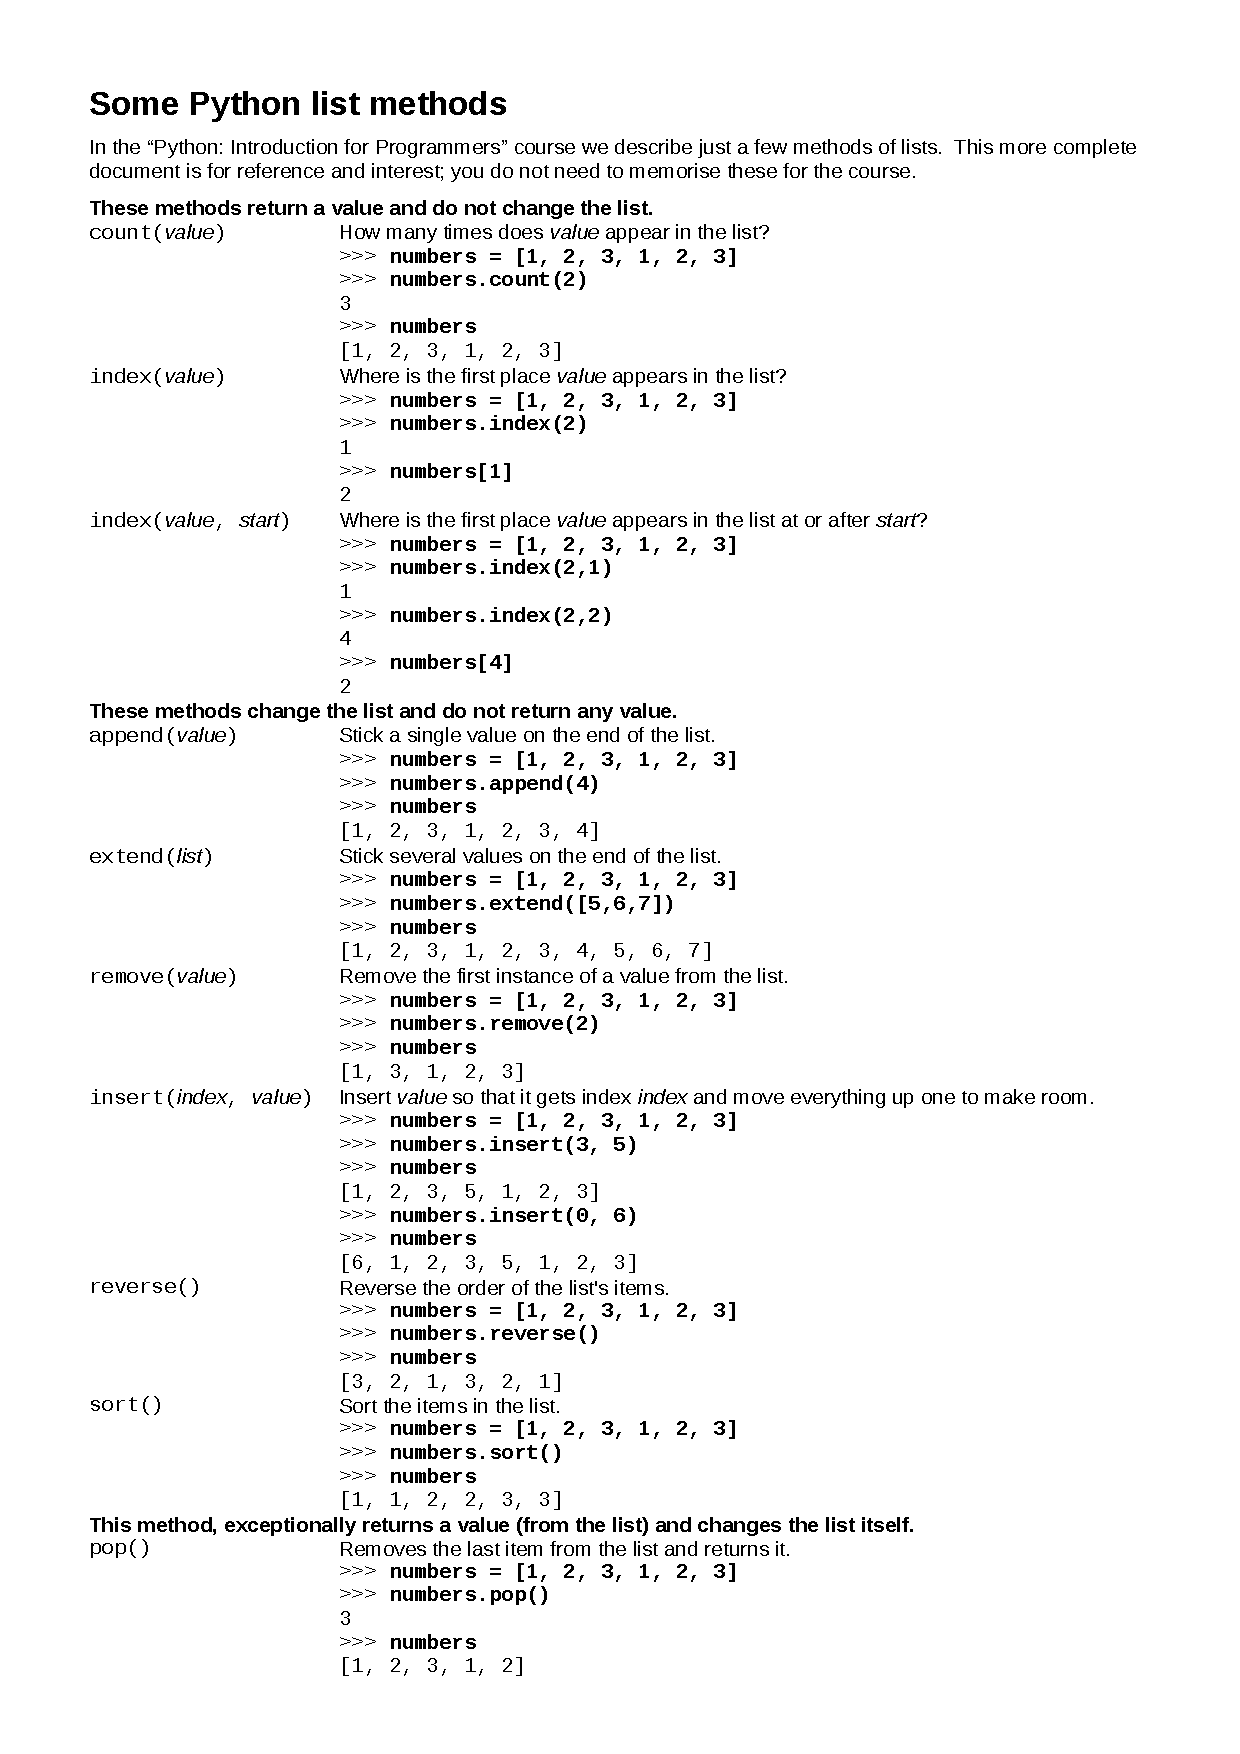
\includepdf[pages={-}]{notes/list_methods.pdf}

\chapter{String Formattig}
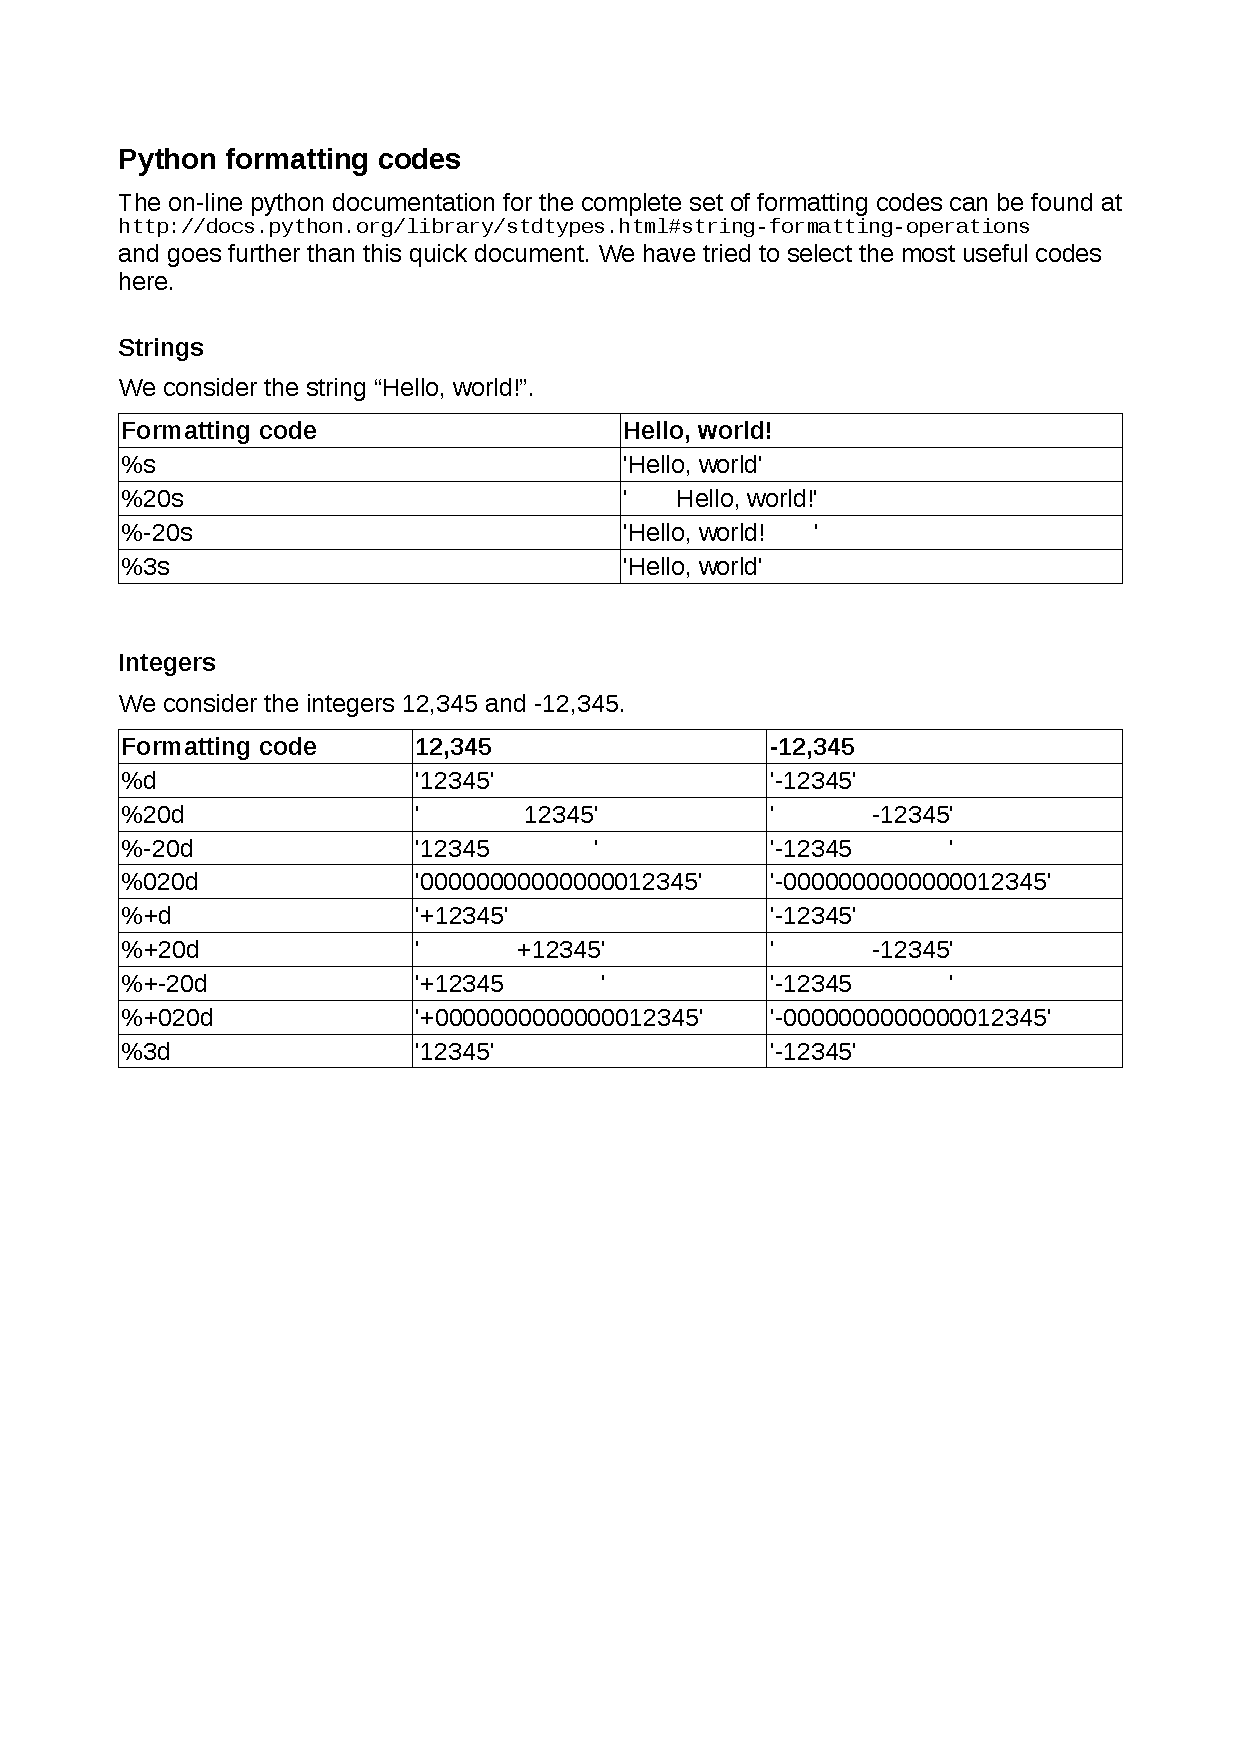
\includepdf[pages={-}]{notes/formatting.pdf}

\chapter{Built-in Modules}
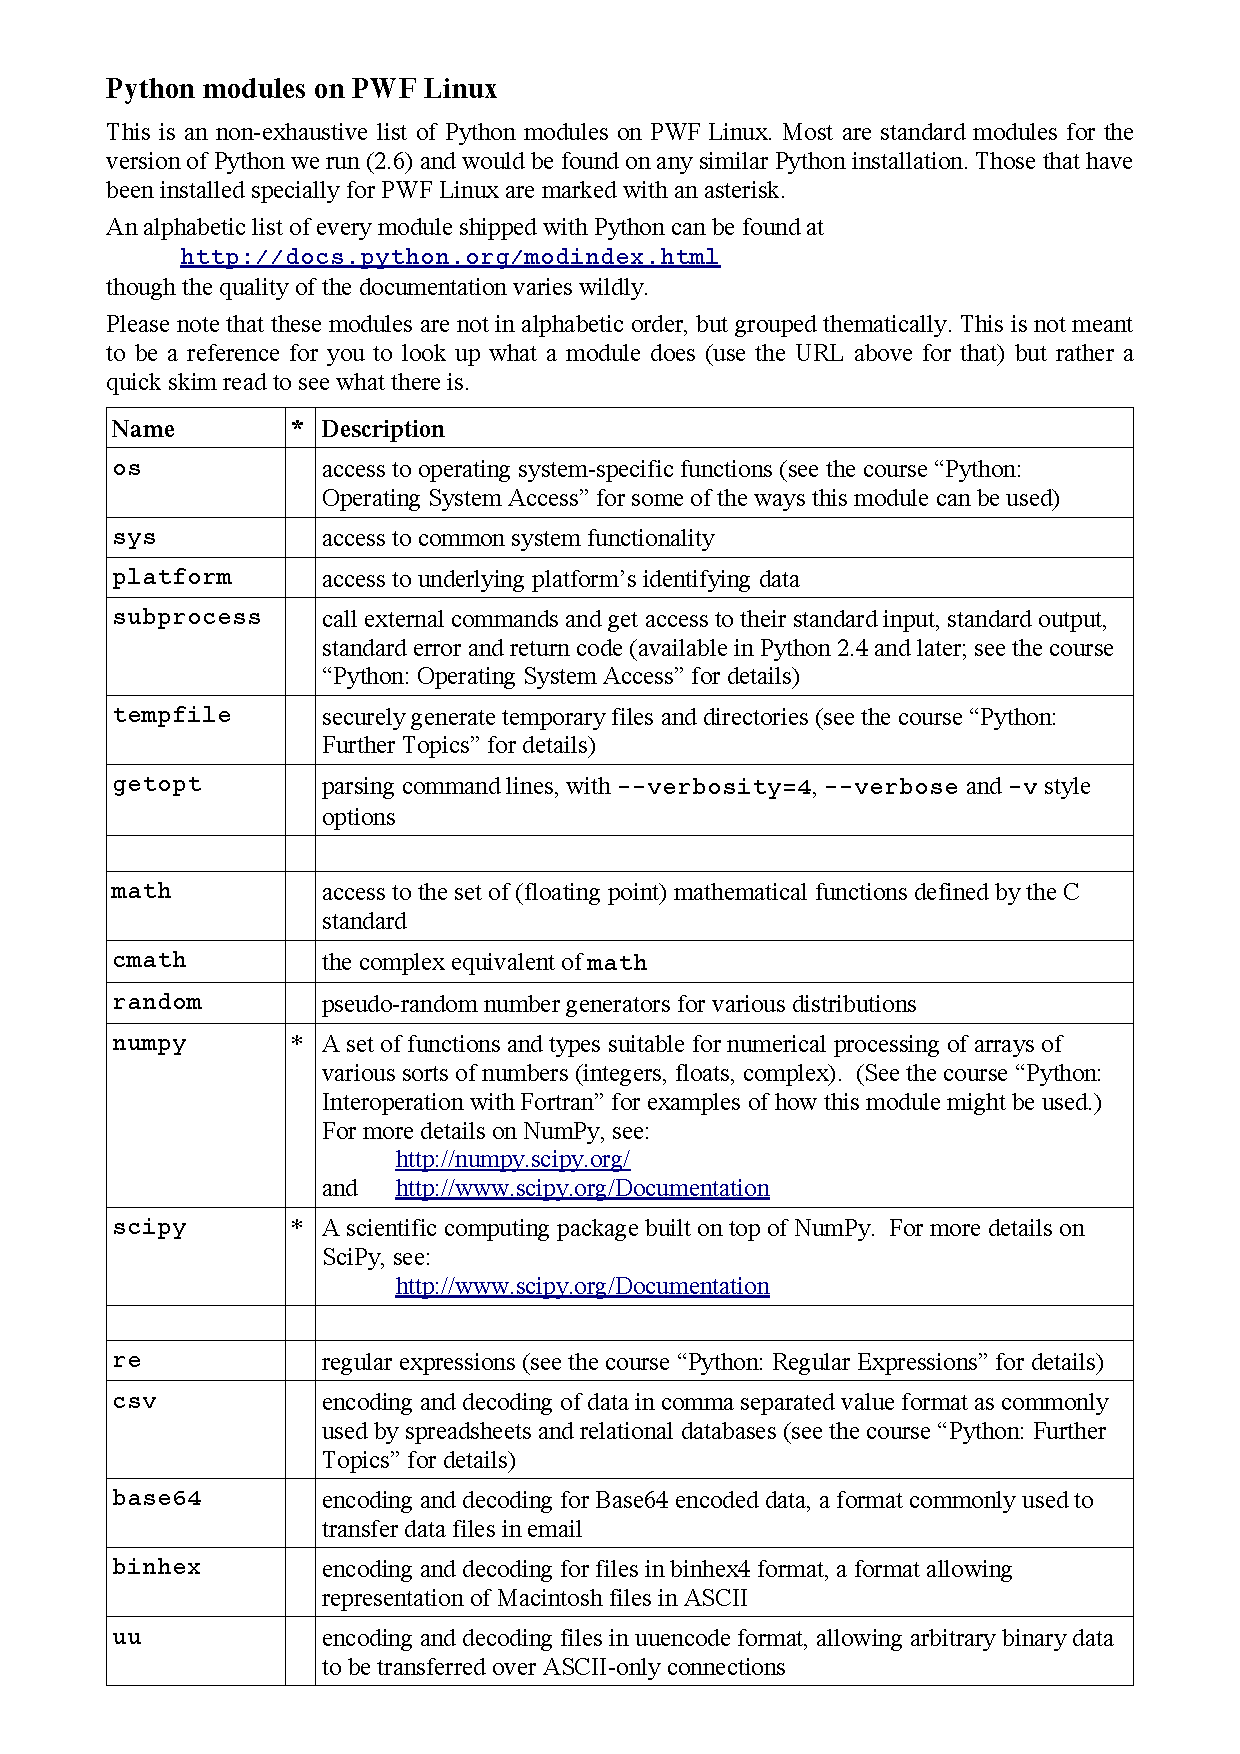
\includepdf[pages={-}]{notes/modules.pdf}

\part{Python Labs}

\chapter{Python Syntax}

\section{Variables and Data Types}
Python was developed to be clear, powerful, and fun to use. We'll start with a quick note on what Python is and how it's used, then we'll jump right into writing code! This course assumes no prior knowledge in Python.

Python is a powerful, flexible programming language you can use in web/Internet development, to write desktop graphical user interfaces (GUIs), create games, and much more. Python is:
\begin{enumerate}
\item High-level, meaning reading and writing Python is really easy—it looks a lot like regular English!
\item Interpreted, meaning you don't need a compiler to write and run Python! You can write it here at Codecademy or even on your own computer (many are shipped with the Python interpreter built in—we'll get to the interpreter later in this lesson).
\item Object-oriented, meaning it allows users to manipulate data structures called objects in order to build and execute programs. We'll learn more about objects later.
\item Fun to use. Python is named after Monty Python's Flying Circus, and example code and tutorials often refer to the show and include jokes in order to make learning the language more interesting.
\end{enumerate}
This course assumes no previous knowledge of Python in particular or programming/computer science in general.

\subsection{Variables}
One of the most basic concepts in computer programming is the variable. A variable is a word/identifier that hangs onto a single value. For example, let's say you needed the number 5 for your program, but you're not going to use it immediately. You can set a variable, say spam, to grab the value 5 and hang onto it for later use, like this:
\begin{lstlisting}
spam = 5
\end{lstlisting}
Declaring variables in Python is easy; you just write out a name/identifier, like spam, and use = to assign it a value, and you're done!

\subsubsection{INSTRUCTIONS}
Set the variable my\_variable to the value 10.

\subsection{Data Types}
Great! We can now summon the value 10 by calling out the name my\_variable whenever we need it.

In this case, the data type of my\_variable is an integer (a positive or negative whole number). There are three data types in Python that are of interest to us at the moment: integers, floats (fractional numbers written with a decimal point, like 1.970), and booleans (which can be True or False).

Computer programs, in large part, are created to manipulate data. Therefore, it's important to understand the different types of data (or "datatypes") that we can incorporate into our programs.

Never use quotation marks (' or ") with booleans, and always capitalize the first letter! Python is case-sensitive (it cares about capitalization). We'll use quotation marks when we get to strings, which we'll cover in the next unit.

\subsubsection{INSTRUCTIONS}
Set the following variables to the corresponding values:
\begin{itemize}
\item my\_int to the value 7
\item my\_float to the value 1.23
\item my\_bool to the value True
\end{itemize}

\subsection{You've Been Reassigned}
Great work. You now know how to declare variables in Python and set them to different values, and you've learned about three different types of values: integers, floats, and booleans.

You can reassign a variable at any point. If you first set my\_int to 7 but later want to change it to 3, all you have to do is tell Python my\_int = 3, and it'll change the value of my\_int for you.

Try it and see!

\subsubsection{INSTRUCTIONS}
Change the value of my\_int from 7 to 3 in the editor.


\section{Whitespace and Statements}
Now that you're getting the hang of variables, values, and assignment (think of them like the subjects, objects, and verbs of English sentences), let's take a look at whitespace and statements: the sentences of our new Python language.

\subsection{What's a Statement?}
You can think of a Python statement as being similar to a sentence in English: it's the smallest unit of the language that makes sense by itself. Just like "I," "like," and "Spam" aren't statements by themselves, but "I like Spam" is, variables and data types aren't statements in Python, but they are the building blocks that form them.

To continue the sentence analogy, it's clear that we also need a kind of punctuation to make it obvious where one statement ends and another begins. If you're familiar with JavaScript, you know that statements end with a semicolon (;). In Python, statements are separated by whitespace. Just like you can't toss around semicolons wherever you want in JS, you can't throw whitespace around in Python.

This may take some getting used to, especially if you're coming from a programming language where whitespace doesn't matter.

\subsubsection{INSTRUCTIONS}
Don't worry about understanding the code on the right; just hit "run" to see what happens.
You should see an error message due to badly formatted code. We'll fix it in the next exercise!

\begin{lstlisting}
def spam():
	eggs = 12
	return eggs
        
print spam()
\end{lstlisting}

\subsection{Whitespace Means Right Space}
Notice the error you got when you ran the code in the editor:

IndentationError: expected an indented   block
You'll get this error whenever your Python whitespace is out of whack. (If you've studied JavaScript, think of improper whitespace as improper use of ; or {}.) When your punctuation's off, your meaning can change entirely:

The peasant said, "The witch turned me into a newt!"
"The peasant," said the witch, "turned me into a newt!"
See what we mean?

\subsubsection{INSTRUCTIONS}
Properly indent the code to the right by hitting the spacebar key on your keyboard four times on line 2 (before eggs) and another four times on line 3 (before return). Click "run" once you've done this.

\subsection{A Matter of Interpretation}
In the introduction to this unit, we mentioned that Python is an interpreted language (meaning it runs using an interpreter). In the context of Codecademy, the interpreter is the console/output window in the lower right corner of the page.

For now, think of the interpreter as a program that takes the code you write, checks it for syntax errors, and executes the statements in that code, line by line. It works as a go-between for you and the computer and lets you know the result of your instructions to the machine.

\subsubsection{INSTRUCTIONS}
Tell Python to assign the value True to the variable spam and False to the variable eggs.

\section{Comments}
Good comments make programs more readable and will help you diagnose problems when they arise. Get in the habit of commenting up your code!

\subsection{Single Line Comments}
Single Line Comments
You may have noticed the instructions in the editor that begin with a \# (pound or hash) symbol. These lines of code are called comments, and they aren't read by the interpreter—they don't affect the code at all. They're plain English comments written by the programmer to provide instructions or explain how a particular part of the program works.

Since this improves the readability of your code tremendously (and will help you debug programs more quickly, since you'll be able to tell at a glance what each part of the program is supposed to do), we encourage you to comment on your code whenever its purpose isn't immediately obvious.

\subsubsection{INSTRUCTIONS}
Write a comment on line 1 in the editor. Make sure it starts with \#! (It can say anything you like.)

\subsection{Multi-Line Comments}
Sometimes you have to write a really long comment. \# will only work across a single line, and while you could write a multi-line comment and start each line with \#, that can be a pain.

If you want to write a comment across multiple lines, you can include the whole block in a set of triple quotation marks, like so:
\begin{lstlisting}
"""I'm a lumberjack and I'm okay
I sleep all night and I work all day!"""
\end{lstlisting}

\subsubsection{INSTRUCTIONS}
Write a multi-line comment in the editor. Include whatever text you want!

\section{Math Operations}
If all we could do in Python were declare variables and write comments, it wouldn't be very exciting. Thankfully, that's not the case—we can combine and manipulate data to create powerful, flexible programs to suit our needs.

\subsection{Arithmetic Operators}
Python's statements aren't limited to simple expressions of assignment like spam = 3; they can also include mathematical expressions using arithmetic operators.

There are six arithmetic operators we're going to focus on:
\begin{itemize}
\item Addition (+)
\item Subtraction (-)
\item Multiplication (*)
\item Division (/)
\item Exponentiation (**)
\item Modulo (\%)
\end{itemize}

\subsubsection{INSTRUCTIONS}
Let's start with addition. Set the variable count\_to to the sum of 1 + 2.

\subsection{Subtraction}
Good! Now let's try subtraction.

\subsubsection{INSTRUCTIONS}
We've clearly counted too far with our count\_to—we've gotten to five but want count\_to to be smaller. Tell Python to reassign count\_to to 5 - 2.

\subsection{Multiplication}
Perfect! Now let's try a little multiplication.

\subsubsection{INSTRUCTIONS}
The Knights Who Say "Ni!" have only said "Ni!" twice. Let's make it twenty times by multiplying 2 * 10.

\subsection{Division}
On second thought, 20 "Ni!"s might be a bit much. Let's use division to get it down to 5.

\subsubsection{INSTRUCTIONS}
Set the value of ni to 5 (that is, 20 / 4).

\subsection{Exponentiation}
Excellent job!

All the arithmetic operations you've done so far have probably either been intuitive or have resembled work you've done in other programming languages (such as JavaScript). Exponentiation, however, might be a new one, so it bears some explaining.

The ** operator raises the first number, the base, to the power of the second number, the exponent. So if you type 2 ** 3, you get 8 (2 ** 3 is the same as 2 * 2 * 2, both of which equal 8). 5 ** 2 = 25, 2 ** 4 = 16, and so on.

\subsubsection{INSTRUCTIONS}
Our lumberjack is super hungry and wants 100 eggs. Set eggs to 100 using exponentiation.

\subsection{Modulo}
Impressive! That was a lot of eggs. Hope you left room for spam!

Our final arithmetic operator is modulo (also called modulus). Modulo returns the remainder left over by integer division. So, if you ask the Python interpreter to evaluate 5 \% 2, it will return 1 (since 2 goes into 5 evenly two times, with 1 left over). 10 \% 5 is 0, 113 \% 100 is 13, and so on.

\subsubsection{INSTRUCTIONS}
Turns out you did leave room for spam—but not much! Set spam equal to 1 using modulo. You can use any two numbers that will leave a remainder of 1 to do this.

\section{Review}
\subsection{Bringing It All Together}
Nice work! So far you've learned about the following in Python:
\begin{itemize}
\item Variables, which are ways to store values for later use;
\item Data types (such as integers, floats, and booleans);
\item Whitespace (and why it's significant!);
\item Statements (and how Python statements are like statements in regular English);
\item Comments (and why they're good for your code!); and
\item Arithmetic operations (including +, -, *, /, **, and %).
\end{itemize}

\subsubsection{INSTRUCTIONS}
Let's put all our knowledge to work.
\begin{itemize}
\item Write a single-line comment on line 1. It can be anything! (Make sure it starts with \# !)
\item Declare a variable, monty, and set it equal to True.
\item Declare another variable, python, and set it equal to 1.234.
\item Declare a third variable, monty\_python, and set it equal to python squared.
\end{itemize}

\section{Project: Tip Calculator}
\subsection{Your Favorite Meal}
This project is designed to complement Unit 1: Python Syntax. It assumes familiarity with only the material covered in that course.

You've just feasted on a truly delicious meal of Spam and eggs. The diner's computer is down, however, so you'll need to compute the cost of your meal yourself.

Here's how it'll break down:
\begin{itemize}
\item Cost of meal: \$44.50
\item Restaurant tax: 6.75\%
\item Tip: 15\%
\end{itemize}

You'll want to apply the tip to the overall cost of the meal (including tax).

\subsubsection{INSTRUCTIONS}
First, let's declare a variable meal and assign it the value 44.50.

\subsection{The Tax}
Good! Now let's create a variable for the tax percentage.

The tax on your meal at this diner is 6.75\%. Because we'll be multiplying with floats and not percentages, however, you'll have to divide 6.75 by 100 in order to get the decimal form of the number. Do you understand why? (See the Hint if you're not sure.)

\subsubsection{INSTRUCTIONS}
Create the variable tax and set it equal to the decimal value of 6.75%.

\subsection{The Tip}
Nice work! You received good service at this diner, so you'd like to leave a 15\% tip on top the cost of the meal (including tax).

Before we compute the tip for your overall bill, let's set a variable for the tip (15\%). Again, this is a percentage, so you'll need to divide 15.0 by 100 in order to get the decimal form of the tip.

\subsubsection{INSTRUCTIONS}
Set the variable tip to 15\% (in decimal form!) on line 5. (You can just type 0.15 directly, if you like.)

\subsection{Reassign in a Single Line}
Okay! We've got the three variables we need to perform our calculation, and we know a bunch of arithmetic operators that will be able to help us out.

We saw in Lesson 1 that we could reassign a variable when needed—for example, we could say spam = 7 at one point in the program, then later change our minds and say spam = 3.

\subsubsection{INSTRUCTIONS}
On line 7 in the editor, reassign meal to the value of itself + itself * tax (this will add the dollar amount of the tax to the cost of the meal). You're completely allowed to reassign a variable in terms of itself!
We're only calculating the cost of meal and tax here—we'll get to the tip soon!

\subsection{Second Verse, Same as the First}
Well, almost the same. Here, we're going to introduce a new variable instead of resetting an existing variable.

Now that meal's got the cost of the food + tax, let's introduce a new variable on line 8, total, that's equal to the new meal + meal * tip. (This should be very similar to what you just did in the last exercise.)

The code on line 10 will nicely format the value of total and will ensure it prints to the console with two numbers after the decimal. (We'll learn all about string formatting, the console, and the print keyword in Unit 2!)

\subsubsection{INSTRUCTIONS}
Assign the variable total to the sum of meal + meal * tip on line 8, then hit "run" to see the total cost of your meal!

\chapter{Strings and Console Output}
This tutorial will show you strings and console output for Python, including creating literal strings, calling a variety of methods of strings, and use the command "print".

\section{Strings}
Strings are an important and extremely common data type in Python. Here, we'll show you how to build and manipulate them!

\subsection{Step One: Strings}
(This course assumes familiarity with the material presented in Lesson 1: Python Syntax.)

Another useful data type in Python is the string. Strings are, well, strings of characters, which is a more formal way of saying they're really just regular English phrases. They can include numbers, letters, and various symbols, like so: "We're \#1!"

A string literal is a string created by literally just writing it down between quotation marks (' ' or " "). You have to use the same type of quotation mark on each end of the string, though—no 'string"s or "string's!

\subsubsection{INSTRUCTIONS}
Assign the string "Always look on the bright side of life!" to the variable brian.

\subsection{Step Two: Things}
Excellent! Let's get a little practice in with strings. Set the following variables to the following phrases:

\subsubsection{INSTRUCTIONS}
\begin{itemize}
\item Set caesar to "Graham"
\item Set praline to "John"
\item Set viking to "Teresa"
\end{itemize}

\subsection{Step Three: Escape!}
Don't get too comfortable: you can't use just any symbol in a string, and some results can only be achieved by special characters. The practice of including these characters in a string requires that these strings be escaped, or marked as unique. The backslash character (\\) does this work for us! We just put it directly before the character we want to escape.

\subsubsection{INSTRUCTIONS}
The string in the editor is broken: the apostrophe in I'm makes Python think the single-quote string ends there. Fix it by escaping the ' in I'm!


\subsection{Access by Offset}
Great work! (By the way, you could also have repaired the string by replacing the single quotes on the ends with double quotes, like this: "Help! Help! I'm being repressed!".)

Remember how we told you that strings were, technically speaking, strings of characters? Wouldn't it be nifty if you could get to each character in a string individually?

Well, you can!

Each character in a string has a subscript or offset, which is a fancy way of saying it has a number attached to it. The number starts at 0 for the leftmost character and increases by one as you move character-by-character to the right. Check out the diagram in the editor!

\subsubsection{INSTRUCTIONS}
\begin{lstlisting}
"""
The string "PYTHON" has six characters,
numbered 0 to 5, as shown below:

+---+---+---+---+---+---+
| P | Y | T | H | O | N |
+---+---+---+---+---+---+
  0   1   2   3   4   5

So if you wanted "Y", you could just type
"PYTHON"[1] (always start counting from 0!)
"""
fifth_letter = 

print fifth_letter
\end{lstlisting}

When you think you've got the hang of the code in the editor, set fifth\_letter equal to the fifth letter of the string "MONTY", like so: "MONTY"[?] (but replace the ? with the correct number).

\section{String Methods}
Modifying strings is useful, but doing it manually is a pain. Thankfully, Python includes a number of methods that can automate this work for us.

\subsection{Four Methods to the Madness}
Great work! Now we're going to talk about some of the methods that are available for use with strings.

We'll explain methods much more in future lessons, but for now, the takeaway is that string methods are pre-built pieces of code that perform specific tasks for strings.

We're going to focus on four string methods in this section:
\begin{itemize}
\item len()
\item lower()
\item upper()
\item str()
\end{itemize}
Let's start with len(), which gets the length of a string!

\subsubsection{INSTRUCTIONS}
Create a variable called parrot and set it to the string "Norwegian Blue" (be sure to include the space and capitalize exactly as shown!).
Then type len(parrot) on line 5, after the word print, like so: print len(parrot). This will print out the number of letters in "Norwegian Blue"!

\subsection{lower()}
Well done! Again, len() returns the length—that is, the number of characters—of the string on which it's called.

Let's say that you don't want any capitalization in your string, though (in this case, "Norwegian Blue"). In this example, it's a tiny amount of work to manually change "Norwegian Blue" to "norwegian blue". But what if you wanted to convert thousands of words to all-lower case? Doing it manually would take forever.

\subsubsection{INSTRUCTIONS}
Python is all about automation! Call lower() on parrot (after the word print) on line 5 in the editor, like so: parrot.lower(). This will make the string all lower-case! (This is different from the way you call len(), and we'll explain the reasoning behind this before this section is over.)

\subsection{upper()}
Perfect! Now your string is 100\% lower case.

\subsubsection{INSTRUCTIONS}
Unfortunately, you just realized you actually need your string to be completely upper case, not lower. Call upper() on parrot (after the word print on line 5) in order to fix this in one fell swoop!

\subsection{str()}
It looks like you're really getting the hang of string methods in Python. In case you're getting a bit bored (and we know adjusting string capitalization isn't the most exciting thing in the world), try the str() method on for size!

The str() method returns a string containing a nicely printable representation of whatever you put between the parentheses. It makes strings out of non-strings! For example,

str(2)
would turn 2 into "2".

\subsubsection{INSTRUCTIONS}
Two steps here:
\begin{itemize}
\item Create a variable pi and set it to 3.14 on line 4.
\item Call str(pi) on line 5, after the print keyword.
\end{itemize}

\subsection{Dot Notation}
As promised, we'll now explain the reason you use len(string) and str(object), but dot notation (e.g. "String".upper()) for the rest.

Dot notation works on string literals ("The Ministry of Silly Walks".upper()) and variables assigned to strings (ministry.upper()) because these methods are specific to strings—that is, they don't work on anything else.

By contrast, len() and str() can work on a whole bunch of different objects (which we'll get to later), so they can't be tied just to strings with dot notation.

\subsubsection{INSTRUCTIONS}
Let's do just a bit more practice. Call len() on ministry on line 4 and upper() on line 5 (do this after the print keyword each time).

\section{Print}
From time to time, we need to see the output of our Python programs. The "print" keyword makes this possible!

\subsection{Printing with String Literals}
The area to the right of these instructions is the editor, which is where we've been writing our code.

Python translates your instructions to instructions the computer can understand with an interpreter. You can think of the interpreter as a little program that ferries information between your Python code and the computer when you click "Save \& Submit Code." The actual window to which the interpreter spits out the output of your code is the console (the window in the upper right).

If you're familiar with JavaScript, then you know that console.log logs the result of evaluating your code to the console; print is Python's version of console.log.

If you haven't studied JavaScript, never fear! All you need to know is that print prints the result of the interpreter's evaluation of your code to the console for you to see.

\subsubsection{INSTRUCTIONS}
Let's start with something simple. Try printing "Monty Python" to the console. The syntax looks like this:
\begin{lstlisting}
print "Your string goes here"
\end{lstlisting}
Don't forget the quotes (' or ")!

\subsection{Printing with Variables}
Great! Now let's combine what we've learned about variables with our new print keyword.

\subsubsection{INSTRUCTIONS}
Declare a variable called the\_machine\_goes and assign it the string value "Ping!" on line 5. Make sure to type "Ping!" exactly as shown—complete with capital "P" and an exclamation point!
Go ahead and print the\_machine\_goes on line 6.

\section{Advanced Printing}
Now that you know how to print output to the console, let's take a look at some of the more complex features supported by "print."

\subsection{String Concatenation}
You know about strings, and you know about arithmetic operators. But did you know some arithmetic operators work on strings?

If you use the + operator between two strings, it concatenates them (glues them together).

print "Monty " + "Python"
will print out "Monty Python"!

\subsubsection{INSTRUCTIONS}
Give it a go in the editor. print the concatenated strings "Spam ", "and ", "eggs" on line 3 to print the string "Spam and eggs" to the console.

\subsection{Explicit String Conversion}
Remember when we talked about the str() method a couple of lessons back, and how it turns non-strings into strings? The fancy name for that process is explicit string conversion.

You're explicitly telling Python, "Hey, I know this isn't a string, but I want to turn it into one." Contrast this with just putting quotes around a sequence of characters to make it a string.

Making a number into a string can let you glue together strings and numbers (which Python normally won't allow). Check it out:

print "I have " + str(2) + " coconuts!"
will print "I have 2 coconuts!"

\subsubsection{INSTRUCTIONS}
\begin{itemize}
\item Run the code as-is. You get an error!
\item Use str() to turn 3.14 into a string, then run the code again.
\end{itemize}

\subsection{String Formatting with \%, Part 1}
Awesome work so far. This is the last new thing to cover before we review!

We saw earlier that you can access individual characters in a string by offset, or, if you want to think about it this way, ID number. (Remember, "PYTHON"[1] is "Y", not "P"!)

Unfortunately, strings in Python are immutable—you can't change them once they're created.

However, there is a way you can work flexibility into your strings, and that's with string formatting. It uses the \% symbol (don't confuse this with modulo!), and you can sort of think of it as a variable for your string.

\subsubsection{INSTRUCTIONS}
Take a look at the code in the editor. What do you think it'll do? Click Save \& Submit Code when you think you know.

\begin{lstlisting}
string_1 = "Camelot"
string_2 = "place"

print "Let's not go to %s. 'Tis a silly %s." % (string_1, string_2)
\end{lstlisting}

\subsection{String Formatting with \%, Part 2}
Did you see that? The \% string formatter replaced the \%s (the "s" is for "string") in our string with the variables in parentheses. (We could have done that by just putting "Camelot" and "place" in parentheses after the string, but we wanted to show you how it works with variables.)

The syntax went like this:
\begin{lstlisting}
print "%s" % (string_variable)
\end{lstlisting}
You can have as many variables (or strings!) separated by commas between your parentheses as you like:
\begin{lstlisting}
print "The %s who %s %s!" % ("Knights", "say", "Ni")
prints "The Knights who say Ni!"
\end{lstlisting}

\subsubsection{INSTRUCTIONS}
For our grand finale, we're showing you a bit of new code. Don't worry if you don't get how it works yet; we'll explain it soon!
For now, replace the \_\_\_s with the form of \% you need to complete your quest: \%s inside the string, and \% to link the string with its arguments. Answer the questions in the console as they pop up!

\begin{lstlisting}
name = raw_input("What is your name?")
quest = raw_input("What is your quest?")
color = raw_input("What is your favorite color?")

print "Ah, so your name is ___, your quest is ___, " \
"and your favorite color is ___." ___ (name, quest, color)
\end{lstlisting}

\section{Review}
Let's take a moment to go over what we've learned.

And Now, For Something Completely Familiar
Great job! You've learned a lot in this unit, including:

What strings are, and how to create them literally (using ' ' or " ") or explicitly (using the str() method);
string methods, such as len(), upper(), and lower();
the print keyword for outputting Python's evaluation of your code to the console; and
advanced printing techniques using \%.
Let's wrap it all up!

\subsection{INSTRUCTIONS}
\begin{enumerate}
\item Create a variable called my\_string and set it to any string you'd like.
\item Go ahead and print its len()gth on line 4.
\item Go for the gold and print its .upper() case version on line 5.
\end{enumerate}

\section{Project: Date and Time}
\subsection{The datetime Library}
In this small project, we'll create a program that experiments with Python's ability to give us the current date and time. This will give you some practice with printing strings, concatenation, and the str() explicit conversion function.

At the end of this section, you'll know how to print the date and time in the following format: mm/dd/yyyy hh:mm:ss.

On line 1, notice the statement from datetime import datetime. Importing special functionality into your programs will be covered in Unit 4's discussion of the import statement.

For now, just know that we're telling the Python interpreter to give our program the ability to retrieve the current date and time.

In the next exercise, we'll cover how to explicitly retrieve this information!

\subsubsection{INSTRUCTIONS}
\begin{lstlisting}
from datetime import datetime
\end{lstlisting}

\subsection{Getting the Current Date and Time}
To retrieve the current date and time, we can use a function called datetime.now() to get that information.

In a later course, you'll learn all about functions. For now, just know that datetime.now() calls on a piece of code that comes with Python that figures out the current date and time for us.

\subsubsection{INSTRUCTIONS}
\begin{enumerate}
\item Create a variable called now and store the result of datetime.now() in it. We'll use this variable in the next exercise.
\item Go ahead and print the value of the variable now.
\end{enumerate}

\subsection{Extracting Information}
Notice how we got an output of the form 2012-07-19 12:50:53.180759. That's pretty ugly.

Let's examine how to extract portions of the date and time to eventually print out a "prettier" form of this information.

Let's start by retrieving the month, day, and year from the result of datetime.now(). To do this, we can use our variable now in the following way: current\_year = now.year.

Of course, the variable on the left-hand side of the assignment could be named anything.

The fact that we can extract parts of the date in such an elegant syntax is pretty awesome. As you could guess, we can use a similar syntax to extract the month and day.

Note: Don't worry about the details of the notation now.year. It's called dot notation and it's used to access data from an object. We mentioned this briefly in Unit 2 and will talk much more about objects later.

\subsubsection{INSTRUCTIONS}
Go ahead and print out the current month, day, and year to the console on separate lines.

\subsection{Hot Date}
Great job printing out the date's components! In gearing up for our ultimate goal of printing out mm/dd/yyyy hh:mm:ss, let's tackle adding / slashes to the date's parts.

You might think to do something like:

print now.month, "/", now.day, "/", now.year
However, this would incorrectly give you spaces between the slashes. Hence, the better solution is to use string concatenation (the + operator), covered in Unit 2.

As you'll see, it's not as simple as just using concatenation—mainly because concatenation only works with strings.

When you extract information like now.year, you end up with an integer (a positive or negative whole number). To convert an integer to a string, you can use the str() function. For example, if a variable x had the value 4 and we wanted to convert that into "4", you could type:
\begin{lstlisting}
str(x)
\end{lstlisting}
\subsubsection{INSTRUCTIONS}
Print out the current date in the pretty form of mm/dd/yyyy. It's totally okay if it comes out as m/d/yyyy.

\subsection{Pretty Time}
Nice work! Let's do the same for the parts of the time—namely, the hour, minute, and second.

As you might guess, we can also use our variable now to print out the time information. If you wanted to print out the current hour, you could do:
\begin{lstlisting}
current_hour = now.hour
\end{lstlisting}
Just for clarification, our variable now contains the results of datetime.now(); there's nothing special about naming the variable "now." It's just for convenience!

\subsubsection{INSTRUCTIONS}
Similar to the last exercise, print out the current time in the pretty form of hh:mm:ss. Remember to use string concatenation.
Note: It's also okay if you end up with h:m:s.

\subsection{Grand Finale}
So far, we've managed to prettily print the date and time separately. Let's combine the two!

\subsubsection{INSTRUCTIONS}
Print out the date and time together in the form: mm/dd/yyyy hh:mm:ss
(Note that a space separates the date and time, so you'll need the + operator once more.)

\chapter{Conditionals and Control Flow}
In this course, we'll learn how to create programs that generate different outcomes based on user input!

\section{Introduction to Control Flow}
"Control flow" is the order in which events occur in a program. This section will introduce the concept of control flow and the ways in which it can be altered.

\subsection{Go With the Flow}

(This course assumes familiarity with the material presented in Unit 1: Python Syntax and Unit 2: Strings \& Console Output. From here on out, take for granted that each new course assumes knowledge of the material presented in the previous courses.)

You may have noticed that the Python programs we've been writing so far have had sort of one-track minds. They compute the sum of two numbers or print something to the console, but they don't have the ability to pick one outcome over another—say, add two numbers if their sum is less than 100, or instead print the numbers to the console without adding them if their sum is greater than 100.

Control flow allows us to have these multiple outcomes and to select one based on what's going on in the program. Different outcomes can be produced based on user input or any number of factors in the program's environment. (The environment is the technical name for all the variables—and their values—that exist in the program at a given time.)

\subsubsection{INSTRUCTIONS}

Check out the code in the editor. To help keep you motivated, we've provided a glimpse into the not-so-distant future: the type of program you'll be able to write once you've mastered control flow. Click Save \& Submit Code to see what happens!

\begin{lstlisting}
def clinic():
    print "You've just entered the clinic!"
    print "Do you take the door on the left or the right?"
    answer = raw_input("Type left or right and hit 'Enter'.").lower()
    if answer == "left" or answer == "l":
        print "This is the Verbal Abuse Room, you heap of parrot droppings!"
    elif answer == "right" or answer == "r":
        print "Of course this is the Argument Room, I've told you that already!"
    else:
        print "You didn't pick left or right! Try again."
        clinic()

clinic()
\end{lstlisting}
    
\section{Comparators}
Comparators help programs make decisions by establishing relationships between variables: for instance, which values are greater than, less than, or equal to others.
    
\subsection{Compare Closely!}

Let's not get ahead of ourselves. First, we'll start with the simplest aspect of control flow: comparators. There are six of them, and we're willing to bet at least a few look familiar:
\begin{lstlisting}
    Equal to (==)
    Not equal to (!=)
    Less than (<)
    Less than or equal to (<=)
    Greater than (>)
    Greater than or equal to (>=)
\end{lstlisting}
Note that == is used to compare whether two things are equal, and = is used to assign a value to a variable.

We hope you're familiar with the ideas of greater/less than and greater/less than or equal to. They work exactly as you think they would: they test to see if a number is (or is not) equal to, greater than (or equal to), or less than (or equal to) another number.

(If you're coming from the JavaScript track: there is no === in Python.)

\subsubsection{INSTRUCTIONS}

Let's run through the comparators in the editor. Set each variable to either True or False depending on what you think the result of the evaluation above it will be. For example, 1 < 2 will be True, because one is less than two.

\begin{lstlisting}
# Assign True or False as appropriate on the lines below!

# 17 < 118 % 100
bool_one = 

# 100 == 33 * 3 + 1
bool_two = 

# 19 <= 2**4
bool_three = 

# -22 >= -18
bool_four = 

# 99 != 98 + 1
bool_five = 
\end{lstlisting}

\subsection{Compare... Closelier}

Excellent! It looks like you're comfortable with basic expressions and comparators.

But what about... extreme expressions and comparators?

(This exercise may seem unnecessary to you, but we can't tell you the number of problems caused in programs by incorrect order of operations or reversed >s and <s. Bugs like this can be a serious problem!)

\subsubsection{Instructions}

Let's run through the comparators in the editor one more time (these expressions are more complex than what you saw in the last exercise). Again, set each variable to either True or False depending on what you think the result of the evaluation above it will be.

\begin{lstlisting}
# Assign True or False as appropriate on the lines below!

# 20 + -10 * 2 > 10 % 3 % 2
bool_one = 

# (10 + 17)**2 == 3**6
bool_two = 

# 1**2**3 <= -(-(-1))
bool_three = 

# 40 / 20 * 4 >= -4**2
bool_four = 

# 100**0.5 != 6 + 4
bool_five = 
\end{lstlisting}

\subsection{How the Tables Have Turned}

Nice work!

Based on our comparisons, you've probably guessed that comparisons in Python generate one of two results: True or False. These are instances of a data type we mentioned briefly in Unit 1 called booleans, and they are the only two instances. Things aren't "sort of True" or "Falseish" or "maybe" in Python—they are True or False (and are always capitalized, unlike in JavaScript).

Let's reverse things a bit: we'll supply the boolean value (True or False), and you write an expression that evaluates appropriately.

\subsubsection{Instructions}

For each boolean value in the editor, write an expression that evaluates to that value. Feel free to write expressions that are as simple or as complex as you'd like! Remember, though: simple is better than complex!

Remember, comparators are: ==, !=, >, >=, <, and <=.

\begin{lstlisting}
# Create comparative statements as appropriate on the lines below!

# Make me true!
bool_one = 

# Make me false!
bool_two = 

# Make me true!
bool_three = 

# Make me false!
bool_four = 

# Make me true!
bool_five = 
\end{lstlisting}

\section{Boolean Operators}
Boolean (or logical) operators help programs make decisions based on whether something AND something else is true, something OR something else is true, or something is NOT true.

\subsection{To Be and/or Not to Be}

Boolean operators (or logical operators) are words used to connect Python statements in a grammatically correct way—almost exactly as in regular English. There are three boolean operators in Python:

    and, which means the same as it does in English;
    or, which means "one or the other OR BOTH" (it's not exclusively one or the other, the way it often is in English);
    not, which means the same as it does in English.

We want to stress this second case to you: if your mom tells you you can have Monty Python and the Holy Grail or Monty Python's Life of Brian, she probably means "one or the other, but not both." Python, on the other hand, would be totally fine with your picking both, so long as you don't pick neither. Python is cooler than your mom.

Boolean operators result (predictably) in boolean values—True or False. We'll go through the three operators one by one.

\subsubsection{Instructions}

Before we get started with and, take a look at the truth table in the editor. (This is for those of you who like to see the bigger picture before we dive into the details.) Don't worry if you don't completely get it yet—you will by the end of this section!

\begin{lstlisting}
"""
     Boolean Operators
---------------------------
True and True is True
True and False is False
False and True is False
False and False is False

True or True is True
True or False is True
False or True is True
False or False is False

Not True is False
Not False is True

"""
\end{lstlisting}

\subsection{And}

The boolean operator and only results in True when the expressions on either side of and are both true. An expression is any statement involving one or more variables and operators (arithmetic, logical, or boolean). For instance:

1 < 2 and 2 < 3 results in True because it is true that one is less than two and that two is less than three.

1 < 2 and 2 > 3 results in False because it is not true that both statements are true—one is less than two, but two is not greater than three.

\subsubsection{Instructions}

Let's practice a bit with and. Assign the boolean values beneath each expression as appropriate. This may seem overkill, but remember: practice makes perfect.

\begin{lstlisting}
# Assign True or False as appropriate on the lines below!

# False and False
bool_one = 

# -(-(-(-2))) == -2 and 4 >= 16**0.5
bool_two = 

# 19 % 4 != 300 / 10 / 10 and False
bool_three = 

# -(1**2) < 2**0 and 10 % 10 <= 20 - 10 * 2
bool_four = 

# True and True
bool_five = 
\end{lstlisting}

\subsection{Or}
The boolean operator or only returns True when either (meaning one, the other or both!) of the expressions on each side of or are true. (It's only False when both expressions are False.) For example:

    1 < 2 or 2 > 3 is True, even though two is not greater than three;
    1 > 2 or 2 > 3 is False, because it is neither the case that one is greater than two nor that two is greater than three.

\subsubsection{Instructions}

Time to practice with or!

\begin{lstlisting}
# Assign True or False as appropriate on the lines below!

# 2**3 == 108 % 100 or 'Cleese' == 'King Arthur'
bool_one = 

# True or False
bool_two = 

# 100**0.5 >= 50 or False
bool_three = 

# True or True
bool_four = 

# 1**100 == 100**1 or 3 * 2 * 1 != 3 + 2 + 1
bool_five = 
\end{lstlisting}

\subsection{Not}

The boolean operator not returns True for false statements and False for true statements. Remember, the only two boolean values are True and False!

For example:

not False will evaluate to True, as will not 40 > 41. Applying not to expressions that would otherwise be true makes them False.

\subsubsection{Instructions}

Last but not least, let's get some practice in with not.
\begin{lstlisting}
# Assign True or False as appropriate on the lines below!

# not True
bool_one = 

# not 3**4 < 4**3
bool_two = 

# not 10 % 3 <= 10 % 2
bool_three = 

# not 3**2 + 4**2 != 5**2
bool_four = 

# not not False
bool_five = 
\end{lstlisting}

\subsection{This and That (or This, But Not That!)}

Fun fact: boolean operators can be chained together!

It's important to know that boolean operators are not evaluated straight across from left to right all the time; just like with arithmetic operators, where / and * are evaluated before + and - (remember Please Excuse My Dear Aunt Sally?), there is an order of precedence or order of operations for boolean operators. The order is as follows:

    not is evaluated first;
    and is evaluated next;
    or is evaluated last.

This order can be changed by including parentheses (()). Anything in parentheses is evaluated as its own unit.

For instance, True or not False and False returns True. Can you see why? If not, check out the Hint.

Best practice: always use parentheses (()) to group your expressions to ensure they're evaluated in the order you want. Remember: explicit is better than implicit!

\subsubsection{Instructions}

Go ahead and assign True or False as appropriate for bool\_one through bool\_five. No math in this one!

\begin{lstlisting}
# Assign True or False as appropriate on the lines below!

# False or not True and True
bool_one = 

# False and not True or True
bool_two = 

# True and not (False or False)
bool_three = 

# not not True or False and not True
bool_four = 

# False or not (True and True)
bool_five = 
\end{lstlisting}

\subsection{Mix 'n Match}

Great work! We're almost done with boolean operators.

\subsubsection{Instructions}

Finally, let's try it the other way 'round—we'll provide the expected result (True or False), and you use any combination of boolean operators you want to achieve that result.

Remember, the boolean operators are and, or, and not.

\begin{lstlisting}
# Use boolean expressions as appropriate on the lines below!

# Make me false!
bool_one = 

# Make me true!
bool_two = 

# Make me false!
bool_three = 

# Make me true!
bool_four = 

# Make me true!
bool_five = 
\end{lstlisting}

\section{If, Else and Elif}
"If," "else," and "elif" are conditional statements that round out the process by which Python programs make decisions—for example, "if there's Spam, eat it! If not, watch TV."
    
\subsection{Conditional Statement Syntax}

Remember when we showed you that whitespace in Python is significant? If not, write this down: whitespace in Python is significant. If you've learned any JavaScript here on Codecademy, you know that the block of code an if statement executes is bound by curly braces ({}). In Python, whitespace (tabs or spaces) does this work for us.

Here's an example of if statement syntax in Python:

if 8 < 9:
    print "Eight is less than nine!"

if is always followed by an expression, which is followed by a colon (:). The code block (the code to be executed if the expression evaluates to True) is indented four spaces.

This is also true for elif and else (which we'll get to in a moment). The full syntax would look something like this:

if 8 < 9:
    print "I get printed!"
elif 8 > 9:
    print "I don't get printed."
else:
    print "I also don't get printed!"

\subsubsection{Instructions}

Here's a piece of code that should look familiar: it's a snippet from the example we showed you in 1.1, "Introduction to Control Flow." If you think the print statement will print to the console, set response equal to 'Y'; otherwise, set response equal to 'N'.

\begin{lstlisting}
response = 

answer = "Left"
if answer == "Left":
    print "This is the Verbal Abuse Room, you heap of parrot droppings!"
    
# Will the above print statement print to the console?
# Set response to 'Y' if you think so, and 'N' if you think not.
\end{lstlisting}

\subsection{If You're Having...}

Let's get some practice in with if statements. Remember, the syntax looks like this:

\begin{lstlisting}
if expression:
    # block line one
    # block line two
    # et cetera
\end{lstlisting}

\subsubsection{Instructions}

Write two if statements in the editor: one that returns True, and a second that returns False. Use any expressions you like! (Don't worry about def and return just yet—we'll cover those in the next unit.)

\begin{lstlisting}
# Write your two if statements below!

def true_function():
    if                # Fill in your if statement here!
        return        # Make sure this returns True

def false_function():
    if                # Fill in your if statement here!
        return        # Make sure this returns False
\end{lstlisting}

\subsection{Else Problems, I Feel Bad for You, Son...}

The else statement in Python is the complement to the if statement. While an if statement will return control of the program to the next line of code after the if code block even if there's no else statement, it's considered a good habit to pair each if with an else.

An if/else pair says to Python: "If this expression is true, run this indented code block; otherwise, run this code after the else statement."

Remember when we said "set response equal to 'Y', otherwise, set it to 'N'" in the first exercise of this section? That was a kind of if/else statement!

\subsubsection{Instructions}

Complete the else statements to the right. Remember to capitalize your booleans, and note the indentation for each line! It's important.

\begin{lstlisting}
# Write your two else statements below!
answer = "'Tis but a scratch!"

def black_knight():
    if answer == "'Tis but a scratch!":
        return True
    else:             # Fill in your else statement here!
        return        # Make sure this returns False

def french_soldier():
    if answer == "Go away, or I shall taunt you a second time!":
        return True
    else:             # Fill in your else statement here!
        return        # Make sure this returns False
\end{lstlisting}

\subsection{I Got 99 Problems, But a Switch Ain't One}

"Elif" is short for "else if." It means exactly what it sounds like: "otherwise, if the following code is true, do this!"

If you're coming from JavaScript, you may know that you have two choices when you have a chain of conditional statements: a bunch of else if statements, or a switch statement. Python simplifies this for you: there's only elif.

\subsubsection{Instructions}

Fill in the elif statement in the editor such that it returns True for the answer "I like Spam!"

You'll want to check whether answer equals the "I like Spam!" string after elif.
\begin{lstlisting}
# Write your two elif statements below!
answer = "I like Spam!"

def feelings_about_spam():
    if answer == "I hate Spam!":
        return False
    elif              # Check the answer variable here!
        return        # Make sure this returns True
    else:
        return False
\end{lstlisting}

\section{Review}
Let's take some time to review what we've covered in this unit.
\subsection{The Big If}

Really great work! Here's what you've learned in this unit:
\begin{itemize}
\item Basics of control flow;
\item Comparators (such as >, <, and ==);
\item Boolean operators (and, or, and not);
\item And conditional statements (if, else, and elif).
\end{itemize}

Let's get to the grand finale.
\subsubsection{Instructions}

Write an if statement in the\_flying\_circus(). It must include:
\begin{itemize}
\item and, or, or not;
\item ==, !=, <, <=, >, or >=;
\item an if, elif, AND else statement;
\item it must return True when evaluated.
\end{itemize}

\chapter{Project: PygLatin}
In this project we'll put together all of the Python skills we've learned so far including string manipulation and branching. We'll be building a Pyg Latin translator. (That's Pig Latin for Python Programmers!)

\section{PygLatin Part 1}
This project will put together all the Python concepts we've been learning to build an English to PYg Latin Translator.

\subsection{Break It Down}

When you start a big project like this, it's important to take some time to break the problem into individual steps. Then you can tackle (and test) one step at a time rather than trying to write a huge program all at once!

Let's think about the PygLatin problem. Pig Latin is a language where we take the first letter of a word and put it on the end while also adding a vowel sound. So dog becomes "ogday". What are the steps we need to take?
\begin{enumerate}
\item    Ask the user to input a word in English
\item    Check to make sure the user entered a valid word
\item    Convert the word from English to Pig Latin
\item    Display the translation result
\end{enumerate}

Notice that some of the steps can themselves be broken down into individual steps. For example, we'll want to think through the algorithm for step \#3 before we start coding.

A little bit of time invested in thinking through the decomposition of and algorithms for your program can save you a LOT of frustration down the road!

Get a piece of paper and work out an algorithm for step \#3 of the project.

\subsubsection{Instructions}

All set? When you're ready to get coding, click the Run button to continue. Since we took the time to write out the steps for our solution, you'll know what's coming next!

\subsection{Ahoy! (or Should I Say Ahoyay!)}

This project will be a workout, so let's warm up by printing a welcome message for our translator users.

\subsubsection{Instructions}

Use Python to print "Welcome to the English to Pig Latin translator!" to the console.

\subsection{Input!}

If we're going to translate an English word into Pig Latin, the first thing we're going to need is a word.

Python can ask for input from the user with the raw\_input command. For example, if you type:
\begin{lstlisting}
name = raw_input("What's your name?")
\end{lstlisting}
Python will print:
\begin{lstlisting}
What's your name? >
\end{lstlisting}
Once you type something and hit Enter, Python will store whatever you typed in the name variable.
\subsubsection{Instructions}

Below your existing code, prompt the user to enter a word, and store it in a variable called original. The prompt message can be whatever you want!

\subsection{Check Yourself!}

Whenever you ask a user for input, it's a good idea to check the result that you get before you use it in your program.

In this case, we want to make sure that the input is something we can reliably translate into Pig Latin. That is, we want to make sure we got something resembling an English word.

The first thing we can check is that there are characters in our string. Let's check to make sure the string isn't empty. How can we check to make sure that our original variable isn't empty?
\subsubsection{Instructions}

Write an if statement that checks to see if the string is not empty.
\begin{itemize}
\item    If the string is not empty, print the user's word.
\item    Otherwise (else), print "empty" if the string is empty.
\end{itemize}
Make sure you thoroughly test your code. You'll want to make sure you run it multiple times and test both an empty string and a string with characters. When you are confident that your code works, continue on to the next exercise.

\subsection{Check Yourself... Some More}

Great! Now we know we have a non-empty string. Let's be even more thorough, though. After all, a user might try to be tricky and enter something like 8675309 which, since it is numbers not letters, would not make sense in PygLatin.

Let's add to our input validation and make sure that the word the user enters contains only alphabetical characters. You can use the isalpha() function to check this. To check if the string "J123" within a variable x is alphabetical, you could do:
\begin{lstlisting}
x = "J123"
x.isalpha() # False
\end{lstlisting}

\subsubsection{Instructions}

Add onto your if condition to check that the word is also composed of all alphabetical characters. You should end up with a single if-else statement that makes sure original is a non-empty alphabetical string.

Make sure to check both an all-alphabetical string and one with letters and numbers!

\subsection{Pop Quiz!}

Teachers sometimes give pop quizzes to make sure their students are mastering current material. Similarly, when you're working on a big project, you should periodically take time to really put your program to the test.

When you finish one part of your program, it's important to test it multiple times, using a variety of inputs.
\subsubsection{Instructions}

Take some time right now to test your current code. Make sure you try some inputs that should pass the word test and some that should fail. Enter some strings that contain non-alphabetical characters and an empty string.

When you're convinced your code is ready to go, click Save \& Submit Code to move on to the next step!

\section{PygLatin Part 2}
Let's continue to build our PygLatin translator!

\subsection{Ay B C}

Now that we know we have a good word, we can get ready to start translating to Pig Latin! Let's quickly review the rules for translation:
\begin{enumerate}
\item If the original word starts with a vowel, you append the suffix 'ay' to the end of the word.
\begin{lstlisting}
Example: anaconda -> anacondaay
\end{lstlisting}
\item If the original word starts with a consonant, you move the first letter of the word to the end, and then append the suffix 'ay'.
\begin{lstlisting}
Example: python -> ythonpay
\end{lstlisting}
\end{enumerate}
Let's create a variable to hold our translation suffix.
\subsubsection{Instructions}
Create a variable named pyg and set it equal to the suffix 'ay'.

\subsection{Word Up}

Since the translation rules depend on the first letter of the word we are translating, we need to grab it so we can check if it is a consonant or a vowel. To simplify things, we'll also go ahead and make sure that all the letters in our word are lowercase to make things a little easier.

To convert a word to all lowercase letters, we can use lower(). For example, to convert the string value "FOO" in a variable x to lowercase, we could do the following:
\begin{lstlisting}
x = "FOO"
x.lower()  # "foo"
\end{lstlisting}
You'll want to think about where to put the code that you write in this step. It really only makes sense to do these steps if you already know that you have a useable word, so make sure you put this code inside the if/else block.
\subsubsection{Instructions}
\begin{itemize}
\item Convert the variable original to all lowercase letters. Store the result in a variable named word.
\item    Create a new variable called first that holds the first letter of word.
\end{itemize}

\begin{lstlisting}
pyg = 'ay'

original = raw_input('Enter a word:')

if len(original) > 0 and original.isalpha():
    print original
else:
    print 'empty'
\end{lstlisting}

\subsection{E-I-E-I-O}

Now that we have access to the first letter of our word, we need to check to see if it is a vowel or a consonant. Since there are way fewer vowels than consonants, it is easier to explicitly check for a vowel. (The vowels in English are: a, e, i, o and u.)

Again, it only makes sense to do this check if we already know that we have a "good" word (one that isn't empty and is all alphabetical characters). You have a couple of options on how to organize your code.

You could add onto your existing if condition to check that something is a good word and starts with a vowel. But then you'd have to add an elif to check if the word is a good word and starts with a consonant.

In this case, it makes more sense to nest the new if block inside the if part of the existing if/else. This means that the whole if/else that you will create here goes inside the if part of your existing if/else block.

A nested if/else looks like this:

\begin{lstlisting}
if condition:
    if other_condition:
        # Do something
    else:
        # Do something else!
else:
    # Do yet another thing

\end{lstlisting}

\subsubsection{Instructions}

Add a new if/else block nested inside of your existing one.

The new if should check to see if the first letter of word is a vowel. If it is, your code should print "vowel". If the first letter of word is not a vowel, your code should print "consonant".

You can remove the print original line from your code.

\subsection{I'd Like to Buy a Vowel}

Now that we have the logical structure in place to check for a vowel, let's put in the code to do the actual translation.

Remember that if a word starts with a vowel, you translate it to Pig Latin by appending our suffix ("ay") to the end of the word.

We'll want to make sure we output the result of the translation so we can check our work.
\subsubsection{Instructions}

Create a new variable called new\_word that contains the result of appending 'ay' to the end of word. (Remember that this suffix is stored in the variable pyg.)

Make sure you are only doing this in the case where the word starts with a vowel. Don't worry about the consonants just yet, we'll get to them in the next step!

After the translation, print the new word so you can check your work. (This should replace the print 'vowel' bit of your code.) Make sure to test your code with a word that starts with a vowel!

\subsection{Almost Oneday!}

Now that we have the vowel case working, all that's left is to tackle the consonant case (our inner else, since a letter can only be a consonant or a vowel).

The rule for translation here is a little trickier. You have to remove the first letter from the word, move it to the end, and then append the 'ay' suffix.

The most appropriate way to get the remainder of the string after removing the first letter is to use slicing. If you have a string s, you can get the "slice" of s from i to j using s[i:j]. This gives you the characters from position i to j.

For example, if s = "foo", then s[0:2] gives you "fo". Think about how to use this technique to get the rest of the string minus the first character.

\subsubsection{Instructions}

Inside the else part of your if/else block that checks the first letter of the word, set the new\_word variable equal to the translation result for a word that starts with a consonant.

Replace the print 'consonant' bit with print new\_word. Make sure to test your code with a word that starts with a consonant!

\subsection{Testing, Testing, is This Thing On?}

Yay! You should have a fully functioning Pig Latin translator. Just to make sure everything is working smoothly, make sure you test your code thoroughly.

You'll also want to go back through and take out any print statements that you were using to help debug intermediate steps of your code. While you're cleaning things up—now might be a good time to add some comments too! Making sure your code is clean, commented, and fully functional is just as important as writing it in the first place.

\subsubsection{Instructions}

When you're sure your translator is working just the way you want it, click Save \& Submit Code to finish this project.

\begin{lstlisting}
pyg = 'ay'

original = raw_input('Enter a word:')

if len(original) > 0 and original.isalpha():
    print original
else:
    print 'empty'
\end{lstlisting}

\chapter{Functions}
A function is a reusable section of code written to perform a specific task in a program. We gave you a taste of functions in Unit 3; here, you'll learn how to create your own.

\section{Introduction to Functions}
It's... functions!
\subsection{Documentation: a PSA}

Codecademy is a great educational tool—you can think of it as an online classroom for learning a programming language. It's important to remember, however, that the emphasis should be on your approach to problems and learning to think like a programmer, and not on memorizing every single method or nuance of syntax to be found in a given programming language.

Think of it this way: if you're going to Germany, you wouldn't say to yourself, "Hey, I took a year of German in college, I don't need my dictionary or translation app!" You would totally bring those things to help remind you of vocabulary and syntax in case you were to get stuck; even professional translators keep dictionaries and grammar guides handy for unusual words and tricky constructions.

Much like professional translators, professional programmers refer to documentation when they're not clear on best practices, forget how a certain method works, or need to look up syntax. Python's documentation can be found here. We encourage you to read through it on your own!
\subsubsection{Instructions}

Part of Python's documentation are the PEPs, or "Python Enhancement Proposals." PEP 20, "The Zen of Python," is something of an easter egg hidden in the interpreter (you may have caught us quoting from it in instructional text or hints).

Type import this in the editor to see what happens (we'll learn about the import keyword later in this lesson). Scroll to read all the text output to the console.

\subsubsection{What Good are Functions?}

A function is a reusable section of code written to perform a specific task in a program. You might be wondering why you need to separate your code into functions, rather than just writing everything out in one giant block. You might have guessed the answer(s) already, but here are some of the big ones:
\begin{enumerate}
\item    If something goes wrong in your code, it's much easier to find and fix bugs if you've organized your program well. Assigning specific tasks to separate functions helps with this organization.

\item    By assigning specific tasks to separate functions (an idea computer scientists call separation of concerns), you make your program less redundant and your code more reusable—not only can you repeatedly use the same function in a single program without rewriting it each time, but you can even use that function in another program.

\item    When we learn more about objects, you'll find out there are a lot of interesting things we can do with functions that belong to those objects (called methods).
\end{enumerate}
\subsubsection{Instructions}

Check out the code in the editor. If you completed the Tip Calculator project, you'll remember going through and calculating tax and tip in one chunk of program. Here you can see we've defined two functions: tax to calculate the tax on a bill, and tip to compute the tip.

See how much of the code you understand at first glance (we'll explain it all soon). When you're ready, click Save \& Submit Code to continue.

\begin{lstlisting}
def tax(bill):
    """Adds 8% tax to a restaurant bill."""
    bill *= 1.08
    print "With tax: %f" % bill
    return bill

def tip(bill):
    """Adds 15% tip to a restaurant bill."""
    bill *= 1.15
    print "With tip: %f" % bill
    return bill
    
meal_cost = 100
meal_with_tax = tax(meal_cost)
meal_with_tip = tip(meal_with_tax)
\end{lstlisting}

\subsection{Ample Examples}

All right! Now that you know what functions are good for, it's time to see one in action. (Hopefully it's familiar to you!)

You'll see in the editor a variable, length, assigned to the result or output of a function, len(). This function is built into Python (we'll see how to define our own functions in a moment—you got a sneak peek in the last exercise). Here's how the code to the right works:
\begin{enumerate}
\item    It first evaluates the right hand-side of the assignment. To evaluate the function call, it looks at the long string in parentheses.
\item    Since it's a string literal, it doesn't need to be evaluated (that is, it's not an expression that Python has to figure out, like 1 + 1). So, this string is fed directly as an input to the len() function.
\item    len() accepts this input and returns (or outputs) an integer representing the length of the literal string (in this case 45, including spaces and punctuation).
\end{enumerate}
We've tossed in a print statement to show you that the result is, in fact, 45.
\subsubsection{Instructions}

Replace the string literal inside len's parentheses with a stringified version of the number 45. That is, don't just type "45", but actually use a string function to turn 45 into a string.

\section{Function Syntax}
Functions are great for automating tasks you're going to use over and over, or for making it easy to refer to large sections of your program using one specific name. But how are they put together?

\subsection{Function Junction}

Functions are defined using the keyword def (short for "define"). Functions have three parts:

    The header, which includes the def keyword, the name of the function, any arguments the function takes inside parentheses (()), and a colon (:). (We'll get to arguments in the next exercise);
    An optional docstring, which is a triple-quoted, multi-line comment that briefly explains what the function does;
    And the body, which is the code block that describes the procedures the function carries out. The body is indented (much like for if, elif, and else statements).

Here's an example of what the syntax would look like for a simple function, ni\_sayer, that just prints "Ni!" to the console:
\begin{lstlisting}
def ni_sayer():
    """Prints 'Ni!' to the console."""
    print "Ni!"
\end{lstlisting}

(This is not a very good example of a docstring—ideally, the docstring should explain something that isn't blindingly obvious.)
\subsubsection{Instructions}

Time for you to make your own simple function. Go ahead and create a function, spam, that prints the string "Eggs!" to the console. Be sure to use the capitalization and punctuation shown! Don't forget to include a docstring of your own choosing (just remember to enclose it in triple quotes).

\begin{lstlisting}
# Define your spam function starting on line 5. You
# can leave the code on line 11 alone for now--we'll
# explain it soon!






# Define the spam function above this line.
spam()
\end{lstlisting}

\subsection{Call and Response}

Defining a function is all well and good, but it's not much use to you unless you call it. That's the code you saw on line 11 in the previous exercise: when Python saw spam(), it understood that to mean: "Look for the function called spam and execute the code inside it." The parentheses after the function name let Python know that spam is the name of a function.

\subsubsection{Instructions}

We've set up a function, square, in the editor to the right. Call it on the number 10 on line 9 to see what it does! (That is, put 10 between the parentheses of square().)

\begin{lstlisting}
def square(n):
    """Returns the square of a number."""
    squared = n**2
    print "%d squared is %d." % (n, squared)
    return squared
    
# Call the square function on line 9! Make sure to
# include the number 10 between the parentheses.
\end{lstlisting}

\subsection{No One Ever Does}

If a function takes arguments, we say it accepts or expects those arguments. For instance, if the function no\_one takes a single argument, "The Spanish Inquisition", we would say that no\_one expects "The Spanish Inquisition".

Ha!

To be precise, the argument is the piece of code you actually put between the function's parentheses when you call it, and the parameter is the name you put between the function's parentheses when you define it. For instance, when we defined square in the previous exercise, we gave it the parameter n (for "number"), but passed it the argument 10 when we called it.

You can think of parameters as nicknames the function definition gives to arguments, since it doesn't know ahead of time exactly what argument it's going to get.

The syntax for a function that just prints out the argument it expects would look something like the below.

Function definition:
\begin{lstlisting}
def no_one(sentence):
    print sentence
\end{lstlisting}
Calling the function:
\begin{lstlisting}
no_one("The Spanish Inquisition")
\end{lstlisting}
And the console would display:
\begin{lstlisting}
"The Spanish Inquisition"
\end{lstlisting}
which is the value the parameter sentence takes on when you call no\_one and pass the argument "The Spanish Inquisition".
\subsubsection{Instructions}

Make sense? Good! Check out the function in the editor, power. It should take two arguments, a base and an exponent, and raise the first to the power of the second. It's currently broken, however, because its parameters are missing.

Replace the \_\_\_s with the parameters base and exponent and call power on a base of 37 and a power of 4.

\begin{lstlisting}
def power(___, ___):  # Add your parameters here!
    result = base**exponent
    print "%d to the power of %d is %d." % (base, exponent, result)

power()  # Add your arguments here!
\end{lstlisting}

\subsection{Splat!}

Speaking of not knowing what to expect: your functions not only don't know what arguments they're going to get ahead of time, but occasionally, they don't even know how many arguments there will be.

Let's say you have a function, favorite\_actor, that prints out the argument it receives from the user. It might look something like this:

\begin{lstlisting}
def favorite_actor(name):
    """Prints out your favorite actor."""
    print "Favorite actor is: " , name
\end{lstlisting}
This is great for just one actor, but what if you want to print out the user's favorite actors, without knowing how many names the user will put in?

The solution: splat arguments. Splat arguments are an arbitrary number of arguments, and you use them by preceding your parameter with a *. This says to Python, "Hey man, I don't know how many arguments there are about to be, but it could be more than one." The convention is to use *args, but you can use just about any name you like with a * before it.
\subsubsection{Instructions}

Replace the \_\_\_\_\_s in the function to the right with the appropriate code and click Save \& Submit Code to see who your favorite actors are (or, at least, who they should be). Remember to include a * before your parameter (between the parentheses on line 1).

You don't need the * when you replace the \_\_\_\_\_ on line 3—just the parameter name you chose on line 1.

\begin{lstlisting}
def favorite_actors(_____):
    """Prints out your favorite actorS (plural!)"""
    print "Your favorite actors are:" , _____
    
    
favorite_actors("Michael Palin", "John Cleese", "Graham Chapman")
\end{lstlisting}

\subsection{Functions Calling Functions}

So far, we've seen functions that can print text to the console or do simple arithmetic, but functions can be much more powerful than that. For example, it's completely permissible for a function to call another function.
\subsubsection{Instructions}

Check out the two functions in the editor: one\_good\_turn and deserves\_another. The first function adds 1 to number it gets as an argument, and the second adds 2.

In the body of deserves\_another, change the function so that it always adds 2 to the output of one\_good\_turn.

\begin{lstlisting}
def one_good_turn(n):
    return n + 1
    
def deserves_another(n):
    return n + 2
\end{lstlisting}

\subsection{Practice Makes Perfect}

You never really know how to do something until you do it yourself. We're taking the training wheels off now: time for you to define and call functions all on your lonesome. No examples, no code in the editor. Not even a hint! (Well, okay, one hint.)

And while we're thinking of it: you can always practice your functions (or any Python code) in either the scratch pad. Experimenting in the Labs is a great way to reinforce what you've learned in Codecademy lessons.
\subsubsection{Instructions}
\begin{enumerate}
\item    Define a function called cube that takes a number and returns the cube of that number. (Cubing a number is the same as raising it to the third power).

\item    Define a second function called by\_three that takes one number as an argument. If that number is evenly divisible by 3, by\_three should call cube on that number. If the number is not evenly divisible by 3, cube should return False.
\end{enumerate}
So, for example, by\_three should take 9, determine it's evenly divisible by 3, and pass it to cube, who returns 729 (the result of 9**3). If by\_three gets 4, however, it should return False and leave it at that.

    
\section{Importing Modules}
Remember that scene in The Matrix where Neo learns kung fu by downloading a program directly into his brain? Importing modules: just like that.

\subsection{I Know Kung Fu}

Remember import this from the first exercise in this course? That was an example of importing a module. A module is a file that contains definitions—including variables and functions—that you can use. It would clutter up the interpreter to keep all these variables and functions around all the time, so you just import the module you want when you need something from it.
\subsubsection{Instructions}

Before we try any fancy importing, let's see what Python already knows about square roots. On line 3 in the editor, ask Python to
\begin{lstlisting}
print sqrt(25)
\end{lstlisting}
which we would expect to equal five.

\subsection{Generic Imports}

Did you see that? Python said: "NameError: name 'sqrt' is not defined." Python doesn't know what square roots are—yet.

There is a Python module named math that includes a number of useful variables and functions, and (as you've probably guessed) sqrt() is one of those functions. In order to get to it, all you need is the import keyword. When you simply import a module this way, it's called a generic import.

\subsubsection{Instructions}

You'll need to do two things here:
\begin{enumerate}
\item    Type import math on line 2 in the editor, and
\item    Insert math. (that's math, followed by a period) before sqrt(). This tells Python not only to import math, but to get the sqrt() function from within math.
\end{enumerate}
Once you've done this, hit "run" to see what Python now knows.

\subsection{Function Imports}

Nice work! Now Python knows how to take the square root of a number (as well as how to do everything contained in the math module).

Importing the entire math module is kind of annoying for two reasons, though: first, we really only want the sqrt function, and second, we have to remember to type math.sqrt() any time we want to retrieve that function from the math module.

Thankfully, it's possible to import only certain variables or functions from a given module. Pulling in just a single function from a module is called a function import, and it's done using the from keyword, like so:
\begin{lstlisting}
from module import function
\end{lstlisting}
where "module" and "function" are replaced by the names of the module and function you want. The best part is, now you only have to type sqrt() to get the square root of a number—no more math.sqrt()!
\subsubsection{Instructions}

Let's import the sqrt function from math again, only this time, let's only get the sqrt function. (You don't need the () after sqrt in the from math import sqrt bit.)

\subsection{Universal Imports}

Great! We've found a way to handpick the variables and functions we want from the modules that contain them.

What if we want a large selection (or all) of the variables and functions available in a module? We can import module, but there's another option.

When you import math, you're basically saying: "Bring the Math Box to my apartment so I can use all the cool stuff in it." Whenever you want a tool in math, you have to go to the box and pull out the thing you want (which is why you have to type math.name for everything—even though the box is in your apartment, all the cool stuff you want is still in that box).

When you choose from math import sqrt, you're saying: "Bring me only the square root tool from the Math Box, and don't bring the Math Box to my apartment." This means you can use sqrt without reference to math, but if you want anything else from math, you have to import it separately, since the whole Math Box isn't in your apartment for you to dig through.

The third option is to say: "Don't bring the Math Box to my apartment, but bring me absolutely every tool in it." This gives you the advantage of having a wide variety of tools, and since you have them in your apartment and they're not all still stuck in the Math Box, you don't have to constantly type math.name to get what you want.

The syntax for this is:
\begin{lstlisting}
from module import *
\end{lstlisting}
If you're familiar with CSS, you've seen that * can stand for "every selector," and it serves a similar function in Python: it stands in for every variable and function name in a module.
\subsubsection{Instructions}

Use the power of from module import * to import everything from the math module on line 3 of the editor.

\subsection{Here Be Dragons}

Here's something we've learned in life (and not just from programming): just because you can do something doesn't mean that you should.

Universal imports may look great on the surface, but they're not a good idea for one very important reason: they can fill your program with a ton of variable and function names, but without the safety of those names still being associated with the module(s) they came from.

If you have a function of your very own named sqrt and you import math, your function is safe: there is your sqrt and there is math.sqrt, and ne'er the twain shall meet. If you do from math import *, however, you have a problem: namely, two different functions with the exact same name.

Even if your own definitions don't directly conflict with names from imported modules, if you import * from several modules at once, there won't be any way for you to figure out which variable or function came from where. It'd be like having someone dump a ton of random stuff from a bunch of different boxes in your apartment, then throwing the boxes away so you can't even see where the stuff came from.

For these reasons, it's best to stick with either import module and suffer the inconvenience of having to type module.name, or just import specific variables and functions from various modules as needed.

\subsubsection{Instructions}

Line 1 and line 3 in the editor should look familiar to you; line 2 is an example of some of the cool stuff you'll be able to do in future lessons. In a nutshell, this code will show you everything available in the math module.

Click Save \& Submit Code to check it out (you'll see sqrt, along with some other useful things like pi, factorial, and trigonometric functions). Feel free to spend a few minutes playing around with them!



\section{Built-In Functions}

    Just because you didn't define a function for Python doesn't mean it doesn't know it. Python has a number of built-in functions you can use to write all sorts of powerful, elegant programs.

\subsection{On Beyond Strings}

Now that you understand what functions are and how to import modules, it's worth showing you some of the cool functions that are built in to Python (no modules required!).

You already know about some of the built-in functions we've used on (or to create) strings, such as .upper(), .lower(), str(), and len(). These are great for doing work with strings, but what about something a little more analytic?
\subsubsection{Instructions}

Check out the code in the editor. What do you think it'll do? Click Save \& Submit Code when you think you have an idea.

\begin{lstlisting}
def biggest_number(*args):
    print max(args)
    return max(args)
    
def smallest_number(*args):
    print min(args)
    return min(args)

def distance_from_zero(arg):
    print abs(arg)
    return abs(arg)


biggest_number(-10, -5, 5, 10)
smallest_number(-10, -5, 5, 10)
distance_from_zero(-10)
\end{lstlisting}

\subsection{max()}

The max() function takes any number of arguments and returns the largest one. ("Largest" can have odd definitions here, so it's best to use max() on things like integers and floats, where the results are straightforward, and not on other objects, like strings.)

For example, max(1,2,3) will return 3 (the largest number in the set of arguments).
\subsubsection{Instructions}

Try out the max() function on line 3 of the editor. You can provide any number of integer or float arguments to max().

\begin{lstlisting}
# Set maximum to the max value of any set of numbers on line 3!

maximum = 

print maximum
\end{lstlisting}

\subsection{min()}

As you might imagine, min() does the opposite of max()—given a series of arguments, it returns the smallest one.
\subsubsection{Instructions}

Go ahead and set minimum equal to the min() of any set of integers or floats you'd like.

\begin{lstlisting}
# Set minimum to the min value of any set of numbers on line 3!

minimum = 

print minimum
\end{lstlisting}


\subsection{abs()}

The abs() function returns the absolute value of the number it takes as an argument—that is, that number's distance from 0 on an imagined number line, regardless of whether it's positive or negative. For instance, 3 and -3 are both equally far from 0, and thus have the same absolute value: 3. The abs() function always returns a positive value, and unlike max() and min(), it can only take a single number.
\subsubsection{Instructions}

Set absolute equal to the absolute value of -42 on line 3. (This may seem basic, but bear with us—you'll see the value of the exercise soon enough.)

\begin{lstlisting}
# Set absolute to the absolute value of -42 on line 3!

absolute = 

print absolute
\end{lstlisting}

\subsection{type()}

Finally, the type() function does something very interesting: it returns the type of the data it receives as an argument. If you ask Python to do the following:
\begin{lstlisting}
print type(42)
print type(4.2)
print type('spam')
print type({'Name':'John Cleese'})
print type((1,2))
\end{lstlisting}

Python will output:
\begin{lstlisting}
<type 'int'>
<type 'float'>
<type 'unicode'>
<type 'dict'>
<type 'tuple'>
\end{lstlisting}

(The 'unicode' type is a special type of string.)

You're already familiar with integers, floats, and strings; you'll learn about dictionaries and tuples in later lessons.

\subsubsection{Instructions}

Have Python print out the type of an int, a float, and a unicode string in the editor. You can pick any values on which to call type(), so long as they produce one of each.


\section{Review}

    Let's take some time to go over what we've covered in this unit.
\subsection{Review: Functions}

Up until now, the review section of each unit has been a single exercise. As you progress through the Python courses, you'll see longer review sections (starting with this one)—this is to ensure you have ample practice as you're exposed to more (and more complex) aspects of the language.

Okay! Let's review functions. Again, training wheels are off, but feel free to take a peek at earlier exercises if you need a refresher.
\subsubsection{Instructions}

Write a function, shut\_down, that takes one parameter (you can use anything you like; in this case, we'd use s for string). The shut\_down function should return "Shutting down..." when it gets "Yes", "yes", or "YES" as an argument, and "Shutdown aborted!" when it gets "No", "no", or "NO".

If it gets anything other than those inputs, the function should return "Sorry, I didn't understand you."

\subsection{Review: Modules}

Good work! Now let's see what you remember about importing modules (and, specifically, what's available in the math module).
Instructions

Import the math module in whatever way you prefer. Call its sqrt function on the number 13689 and print that value to the console.

\subsection{Review: Built-In Functions}

Perfect! Last but not least, let's review some of the built-in functions you've learned about in this lesson.
\subsubsection{Instructions}

This is a two-parter: first, define a function, distance\_from\_zero, with one parameter (choose any parameter name you like).

Second, have that function do the following:
\begin{enumerate}
\item    Check the type of the input it receives.
\item    If the type is int or float, the function should return the absolute value of the function input.
\item    If the type is any other type, the function should return "Not an integer or float!"
\end{enumerate}

\chapter{Taking a Vacation}
Hard day at work? Rough day at school? Take a load off with a programming vacation!

\section{A Review of Function Creation}
    A quick review of writing functions.
\subsection{Before We Begin}

Before we start the lesson, we are just going to do a quick review of functions in Python. Remember, functions are callable blocks of code that we can use over and over again. Using functions saves us time, lines of code, and confusion when writing long programs.
\subsubsection{Instructions}
For a warm up, write a function called answer that takes no input and returns the value 42.

\subsection{Finding Your Identity}

Unfortunately for us, 42 is not the answer to every question in the universe.
\subsubsection{Instructions}

Write the function identity that takes the input x and returns x. You do not need to call the function.

\subsection{Call Me Maybe?}

Remember that you can call functions to make computationally challenging tasks much easier.
\subsubsection{Instructions}

Call the function cube with an input of 27 on line 4. Print the result to the console after you call the function.
\begin{lstlisting}
def cube(x):
    return x**3

\end{lstlisting}

\subsection{Function and Control Flow}

Remember that functions often have to react differently depending on the input they receive.
\subsubsection{Instructions}

Write a function called is\_even that takes one input, x, and returns the string "yep" if the input is even and "nope" otherwise. You do not need to call the function.

\subsection{Problem Solvers}

This final review exercise will involve applying functions to a real life problem.

Let's try writing a function to solve a traditional math question.

For this exercise, you'll need to import the math module discussed in Unit 4. This can be achieved by typing import math at the top of your program.
\subsubsection{Instructions}

Write a function called area\_of\_circle that takes radius as input and returns the area of a circle. The area of a circle is equal to pi times the radius squared. (Use the math.pi in order to represent Pi.)

\section{Planes, Hotels and Automobiles}
It's vacation time! Let's see how much this trip will cost you!
\subsection{Planning Your Trip}

When planning a vacation, it is very important to know exactly how much you are going to spend. With the aid of programming, this task becomes very easy.

We will break your trip down into 3 main costs and then put them together in one big function at the end.
\subsubsection{Instructions}

First, write a function called hotel\_cost that takes the variable nights as input. The function should return how much you have to pay if the hotel costs 140 dollars for every night that you stay.

\subsection{Getting There}

To get to your location, you are going to need to take a plane ride.
\subsubsection{Instructions}

Below your existing code, write a function called plane\_ride\_cost that takes a string, city, as input. The function should return a different price depending on the location. Below are the valid destinations and their corresponding round-trip prices.
\begin{itemize}
\item "Charlotte": 183
\item "Tampa": 220
\item "Pittsburgh": 222
\item "Los Angeles": 475
\end{itemize}

\subsection{Transportation}

Now when you arrive at your destination, you are going to need a rental car in order for you to get around. Luckily for you, the rental car company you use gives discounts depending on how many days you rent the car.
\subsubsection{Instructions}

Below your existing code, write a function called rental\_car\_cost that takes days as input and returns the cost for renting a car for said number of days. The cost must abide by the following conditions:
\begin{enumerate}
\item    Every day you rent the car is \$40.
\item    If you rent the car for 3 or more days, you get \$20 off your total.
\item    If you rent the car for 7 or more days, you get \$50 off your total. (This does not stack with the 20 dollars you get for renting the car over 3 days.)
\end{enumerate}

\subsection{Pull it Together}

Great! Now that you've got your 3 main costs figured out, it's time to put them together in order to find the total cost of your trip.
\subsubsection{Instructions}

Below your existing code, write a function called trip\_cost that takes two inputs, city and days. city should be the city that you are going to visit and days should be the number of days that you are staying.

Have your function return the sum of the rental\_car\_cost, hotel\_cost, and plane\_ride\_cost functions with their respective inputs.

\subsection{Hey, You Never Know!}

You can't expect to only spend money on the plane ride, hotel, and rental car when going on a vacation. While the above items will cover the majority of your expenses, there also needs to be room for additional costs like fancy food or souvenirs.

The amount of money that you wish to spend on additional luxuries is completely up to you.
\subsubsection{Instructions}

Make it so that your trip\_cost function takes a third parameter, spending\_money. Just modify the trip\_cost function to do just as it did before, except add the spending money to the total that it returns.

\subsection{Plan Your Trip!}
\subsubsection{Instructions}

Now that you have it all together, print out the cost of a trip to "Los Angeles" for 5 days with an extra 600 dollars of spending money.


\section{Return to Base}

    Welcome back home! It's time to see how much you owe.
\subsection{Coming Back Home}

Welcome back home! It looks like you've had an amazing vacation.

Unfortunately for you, one too many drinks and a bit too much time at the casino have put you a bit over-budget.
\subsubsection{Instructions}

Go ahead and print out how far over budget you went if you spent 2734.23 on your trip.
\begin{lstlisting}
def hotel_cost(nights):
    return nights * 140

def plane_ride_cost(city):
    if city == "Charlotte":
        return 183 
    elif city == "Tampa":
        return 220 
    elif city == "Pittsburgh": 
        return 222
    else:
        return 475

def rental_car_cost(days):
    cost = days * 40
    if days >= 7:
        cost = cost - 50
    elif days >= 3:
        cost = cost - 20
    return cost 

def trip_cost(city, days, spending_money):
    return rental_car_cost(days) + hotel_cost(days) + plane_ride_cost(city)

# You were planning on taking a trip to LA
# for five days with $600 of spending money.
print trip_cost("Los Angeles", 5, 600)
\end{lstlisting}

\subsection{Gotta Give Me Some Credit}

Yikes! That is a bit more than you intended to spend. You put your hotel bill on your credit card and now you don't have the money to pay for it up front.

It looks like you're going to have to break it up into monthly payments. Programming might aid you in handling this mess.
\subsubsection{Instructions}

Call the hotel\_cost function with 5 days as the input and store the result in a variable called bill.

\begin{lstlisting}
def hotel_cost(nights):
    return nights * 140

\end{lstlisting}

\subsection{At a Bare Minimum}

First, we need to know what the minimum payment is that you can make each month.

Note that the minimum payment you can make is 2\% of your total balance. So the minimum payment you can make with a rate of 2\% and a balance of 1,000 would be 20 dollars (1000 * 0.02 equals 20.)
\subsubsection{Instructions}

Below your existing code, write a function called get\_min that takes balance and rate as inputs and returns the minimum payment that you can make with your total balance. balance and rate should both be given as numbers and not percentages, so 2\% is 0.02.

Go ahead and print out the minimum payment of your bills with a 2\% rate, as calculated by your get\_min function.

\subsection{Something of Interest}

All credit cards charge interest in proportion to your current balance. It's important that we know exactly how much we still owe after making a payment.
\subsubsection{Instructions}

Write a function called add\_monthly\_interest that takes the input balance and returns your balance with interest added to it.

Assume your interest is 15\%. This means that we need to add on 15\% to whatever balance is passed in!

Note that 1/12th of your interest multiplied by your balance is equal to the amount of interest you pay each month (or at least close, anyway). So, addmonthlyinterest(100) should return 101.25.

\subsection{Paying Up}

Now it's time for you to make a function that computes how much you still owe after every monthly payment.

You'll create the function make\_payment as described below. The function should return how much you still owe after you make an arbitrary payment at the beginning of the month.

Note: you calculate how much you still owe by subtracting your payment from your total balance and then adding interest using your add\_monthly\_interest function.
\subsubsection{Instructions}

Finish the function make\_payment that takes the inputs payment and balance.

Have the function return the string "You still owe: x", with x being the amount that you still owe. Remember to add interest to the final amount!

\begin{lstlisting}
def hotel_cost(nights):
    return nights * 140

bill = hotel_cost(5)

def add_monthly_interest(balance):
    return balance * (1 + (0.15 / 12))

def make_payment(payment, balance):
	
	
    return "You still owe: " + str(new_balance)
\end{lstlisting}

\subsection{Run It}
\subsubsection{Instructions}

To finish up, make a \$100 first payment on your hotel bill using your make\_payment function. Remember that you stayed at the hotel for 5 days.

Finally, print that result to the console!

\begin{lstlisting}
def hotel_cost(nights):
    return nights * 140

bill = hotel_cost(5)

def add_monthly_interest(balance):
    return balance * (1 + (0.15 / 12))

def make_payment(payment, balance):
	
	
    return "You still owe: " + str(new_balance)
\end{lstlisting}

\chapter{Lists and Dictionaries}
Lists and dictionaries are powerful tools you can use to store, organize, and manipulate all kinds of information.
\section{Lists}
    A Python list is just a sequence of pieces of information. You can use lists to store strings, numbers, and more!
\subsection{Introduction to Lists}

Lists are a datatype you can use to store a collection of different pieces of information as a sequence under a single variable name. (Datatypes you've already learned about include strings, numbers, and booleans.)

You can assign items to a list with an expression of the form list\_name = [item\_1, item\_2], with the items in between brackets. A list can also be empty: empty\_list = [].
\subsubsection{Instructions}

The list zoo\_animals has three items (check them out on line 1). Go ahead and add a fourth! Just enter the name of your favorite animal (as a "string") on line 1, after the final comma but before the closing ].

\begin{lstlisting}
zoo_animals = ["pangolin", "cassowary", "sloth", ]
# One animal is missing!

if len(zoo_animals) > 3:
	print "The first animal at the zoo is the " + zoo_animals[0]
	print "The second animal at the zoo is the " + zoo_animals[1]
	print "The third animal at the zoo is the " + zoo_animals[2]
	print "The fourth animal at the zoo is the " + str(zoo_animals[3])
\end{lstlisting}

\subsection{Access by Index}

You can access an individual item on the list by its index. An index is like an address that identifies the item's place in the list. The index appears directly after the list name, in between brackets, like this: list\_name[index].

List indices begin with 0, not 1! You access the first item in a list like this: list\_name[0]. The second item in a list is at index 1: list\_name[1]. Computer scientists love to start counting from zero.
\subsubsection{Instructions}

Write a statement that prints the result of adding the second and fourth items of the list. Make sure to access the list by index!
\begin{lstlisting}
numbers = [5, 6, 7, 8]

print "Adding the numbers at indices 0 and 2..."
print numbers[0] + numbers[2]
print "Adding the numbers at indices 1 and 3..."
# Your code here!

\end{lstlisting}

\subsection{New Neighbors}

A list index behaves like any other variable name! It can be used to access as well as assign values.

You saw how to access a list index like this:
\begin{lstlisting}
zoo_animals[0]
# Gets the value "pangolin"
\end{lstlisting}
You can see how assignment works on line 5:
\begin{lstlisting}
zoo_animals[2] = "hyena"
# Changes "sloth" to "hyena"
\end{lstlisting}

\subsubsection{Instructions}

Write an assignment statement that will replace the item that currently holds the value "tiger" with another animal (as a string). It can be any animal you like.
\begin{lstlisting}
zoo_animals = ["pangolin", "cassowary", "sloth", "tiger"]
# Last night our zoo's sloth brutally attacked the poor tiger and ate it whole.

# The ferocious sloth has been replaced by a friendly hyena.
zoo_animals[2] = "hyena"

# What shall fill the void left by our dear departed tiger?
# Your code here!
\end{lstlisting}

\section{List Capabilities and Functions}
    Great work with lists! Now let's learn about some of the cool things we can do with them.
\subsection{Late Arrivals \& List Length}

A list doesn't have to have a fixed length—you can add items to the end of a list any time you like! In Python, we say lists are mutable: that is, they can be changed.

You can add items to lists with the built-in list function append(), like this:
\begin{lstlisting}
list_name.append(item)
\end{lstlisting}
Check it out: we've appended a string to suitcase on line 2.

You can get the number of items in a list with the len() function (short for "length"), like so:
\begin{lstlisting}
len(list_name)
\end{lstlisting}

\subsubsection{Instructions}

Append three more items to the suitcase list. (Maybe bring a bathing suit?) Then, set list\_length equal to the length of suitcase.

\begin{lstlisting}
suitcase = [] 
suitcase.append("sunglasses")

# Your code here!




list_length = # Set this to the length of suitcase

print "There are %d items in the suitcase." % list_length
print suitcase
\end{lstlisting}

\subsection{List Slicing}

If you only want a small part of a list, that portion can be accessed using a special notation in the index brackets. list\_name[a:b] will return a portion of list\_name starting with the index a and ending before the index b.

If you tell Python my\_list = [0, 1, 2, 3], then my\_list[1:3] will return the list [1, 2], leaving the original list unchanged! Check it out:
\begin{lstlisting}
my_list = [0, 1, 2, 3]
my_slice = my_list[1:3]
print my_list
# Prints [0, 1, 2, 3]
print my_slice
# Prints [1, 2]
\end{lstlisting}

\subsubsection{Instructions}

Use list slicing to make a list called first that's composed of just the first two items from suitcase, a list called middle containing only the two middle items from suitcase, and a list called last made up only of the last two items from suitcase.

\begin{lstlisting}
suitcase = ["sunglasses", "hat", "passport", "laptop", "suit", "shoes"]

first =    # The first two items
middle =   # Third and fourth items
last =     # The last two items
\end{lstlisting}

\subsection{Slicing Lists and Strings}

You can slice a string exactly like a list! In fact, you can think of strings as lists of characters: each character is a sequential item in the list, starting from index 0.

If your list slice includes the very first or last item in a list (or a string), the index for that item doesn't have to be included. Here's an example:
\begin{lstlisting}
my_list[:2]
# Grabs the first two items
my_list[3:]
# Grabs the fourth through last items
\end{lstlisting}
\subsubsection{Instructions}

Assign each variable a slice of animals that spells out that variable's name.

\begin{lstlisting}
animals = "catdogfrog"
cat =    # The first three characters of animals
dog =    # The fourth through sixth characters
frog =   # From the seventh character to the end
\end{lstlisting}

\subsection{Maintaining Order}

You can search through a list with the index() function. my\_list.index("dog") will return the first index that contains the string "dog". An error will occur if there is no such item.

Items can be added to the middle of a list (instead of to the end) with the insert() function. my\_list.insert(4,"cat") adds the item "cat" at index 4 of my\_list, and moves the item previously at index 4 and all items following it to the next index (that is, they all get bumped forward by one).
\subsubsection{Instructions}

Use the index() function to assign duck\_index the index of the string equal to "duck". Then insert the string "cobra" at that index.

\begin{lstlisting}
animals = ["aardvark", "badger", "duck", "emu", "fennec fox"]
duck_index =    # Use index() to find "duck"

# Your code here!



print animals # Observe what prints after the insert operation
\end{lstlisting}

\subsection{For One and All}

If you want to do something with every item in the list, you can use a for loop. If you've learned about for loops in JavaScript, pay close attention! They're different in Python.

Here's the syntax:
\begin{lstlisting}
for variable in list_name:
    # Do stuff!
\end{lstlisting}
A variable name follows the for keyword; it will be assigned the value of each list item in turn. in list\_name designates list\_name as the list the loop will work on. The line ends with a colon (:) and the indented code that follows it will be executed once per item in the list.
\subsubsection{Instructions}

Write a statement in the indented part of the for loop that prints a number equal to 2 * number for every list item.
\begin{lstlisting}
my_list = [1,9,3,8,5,7]

for number in my_list:
    # Your code here
    
\end{lstlisting}

\subsection{More with 'for'}

If your list is a jumbled mess, you may need to sort() it. my\_list.sort() will sort the items in my\_list in increasing numerical/alphabetical order.

It's worth noting that sort() does not return a new list; instead, your existing my\_list is sorted in place (the sorted version replaces the unsorted version).
\subsubsection{Instructions}

Write a for loop that populates square\_list with items that are the square (x ** 2) of each item in start\_list. Then sort square\_list!
\begin{lstlisting}
start_list = [5, 3, 1, 2, 4]
square_list = []

# Your code here!


print square_list
\end{lstlisting}

\section{Dictionaries}

    What if you want to store information using something other than the preset index values of 0, 1, 2, and so on? Dictionaries can do that for you!

\subsection{This Next Part is Key}

A dictionary is similar to a list, but you access values by looking up a key instead of an index. A key can be any string or number. Dictionaries are enclosed in curly braces, like so:

d = {'key1' : 1, 'key2' : 2, 'key3' : 3}

This is a dictionary called d with three key-value pairs. The key 'key1' points to the value 1, 'key2' to 2, and so on.

Dictionaries are great for things like phone books (pairing a name with a phone number), login pages (pairing an e-mail address with a username), and more!
\subsubsection{Instructions}

Print the values stored under the 'Sloth' and 'Burmese Python' keys. Accessing dictionary values by key is just like accessing list values by index:
\begin{lstlisting}
residents['Puffin']
# Gets the value 104

# Assigning a dictionary with three key-value pairs to residents:
residents = {'Puffin' : 104, 'Sloth' : 105, 'Burmese Python' : 106}

print residents['Puffin'] # Prints Puffin's room number

# Your code here!

\end{lstlisting}


\subsection{New Entries}

A new key-value pair in a dictionary is created by assigning a new key, like so:
\begin{lstlisting}
dict_name[new_key] = new_value
\end{lstlisting}
An empty pair of curly braces {} is an empty dictionary, just like an empty pair of [] is an empty list.

The length len() of a dictionary is the number of key-value pairs it has. Each pair counts only once, even if the value is a list. (That's right: you can put lists inside dictionaries!)
\subsubsection{Instructions}

Add at least three key-value pairs to the menu variable, with the dish name (as a "string") for the key and the price (a float or integer) as the value. Here's an example:
\begin{lstlisting}
menu['Spam'] = 2.50
\end{lstlisting}

\begin{lstlisting}
menu = {} # Empty dictionary
menu['Chicken Alfredo'] = 14.50 # Adding new key-value pair
print menu['Chicken Alfredo']

# Your code here: Add some dish-price pairs to menu!




print "There are " + str(len(menu)) + " items on the menu."
print menu
\end{lstlisting}

\subsection{Changing Your Mind}

Like lists, dictionaries are mutable (they can be changed). Items can be removed from a dictionary with the del command:
\begin{lstlisting}
del dict_name[key_name]
\end{lstlisting}
will remove the key key\_name and its associated value from the dictionary.

A new value can be associated with a key by assigning a value to the key, like so:
\begin{lstlisting}
dict_name[key] = new_value
\end{lstlisting}
\subsubsection{Instructions}

Delete the 'Sloth' and 'Bengal Tiger' items from zoo\_animals using del.

Set the value associated with 'Rockhopper Penguin' to anything other than 'Arctic Exhibit'.
\begin{lstlisting}
# key - animal_name : value - location 
zoo_animals = { 'Unicorn' : 'Cotton Candy House',
'Sloth' : 'Rainforest Exhibit',
'Bengal Tiger' : 'Jungle House',
'Atlantic Puffin' : 'Arctic Exhibit',
'Rockhopper Penguin' : 'Arctic Exhibit'}
# A dictionary (or list) declaration may break across multiple lines

# Removing the 'Unicorn' entry. (Unicorns are incredibly expensive.)
del zoo_animals['Unicorn']

# Your code here!




print zoo_animals
\end{lstlisting}

\subsection{It's Dangerous to Go Alone! Take This}

Finally, my\_list.remove(value) will remove the the first item from my\_list that has a value equal to value. The difference between del and .remove() is:
\begin{itemize}
\item    del deletes a key and its value based on the key you tell it to delete.
\item    .remove() removes a key and its value based on the value you tell it to delete.
\end{itemize}

\subsubsection{Instructions}

Final challenge! Add code that modifies the dictionary inventory in the following ways:
\begin{enumerate}
\item    Add a key to inventory called 'pocket'
\item    Set the value of 'pocket' to be a list consisting of the strings 'seashell', 'strange berry', and 'lint'
\item    .sort() the items in the list stored under the 'backpack' key
\item    Remove 'dagger' from the list of items stored under the 'backpack' key
\item    Add 50 to the number stored under the 'gold' key
\end{enumerate}

\begin{lstlisting}
inventory = {'gold' : 500,
'pouch' : ['flint', 'twine', 'gemstone'], # Assigned a new list to 'pouch' key
'backpack' : ['xylophone','dagger', 'bedroll','bread loaf']}

# Adding a key 'burlap bag' and assigning a list to it
inventory['burlap bag'] = ['apple', 'small ruby', 'three-toed sloth']

# Sorting the list found under the key 'pouch'
inventory['pouch'].sort() 
# Here the dictionary access expression takes the place of a list name 

# Your code here!

\end{lstlisting}


\chapter{Project: A Day at the Supermarket}
Let's manage our own supermarket and buy some goods along the way!

\section{Looping with Lists and Dictionaries}
Lean how to use the for loop with lists and dictionaries.
\subsection{BeFOR We Begin}

Before we begin our exercise, we should go over the Python for loop one more time. For now, we are only going to go over the for loop in terms of how it relates to lists and dictionaries. We'll explain more cool for loop uses in later courses.

for loops allow us to iterate through all of the elements in a list from the left-most (or zeroth element) to the right-most element. A sample loop would be structured as follows:

\begin{lstlisting}
a = [1,2,3,4,....]
for x in a: 
    # Do something for every x
\end{lstlisting}

This loop will run all of the code in the indented block under the for x in a: statement. The item in the list that is currently being evaluated will be x. So running the following:
\begin{lstlisting}
for item in [1, 3, 21]: 
    print item
\end{lstlisting}
would print 1, then 3, and then 21. The variable between for and in can be set to any variable name (currently item), but you should be careful to avoid using the word “list” as a variable, since that's a reserved word (that is, it means something special) in the Python language.
\subsubsection{Instructions}
Use a for loop to print out all of the elements in the list names.

\begin{lstlisting}
names = ["Adam","Alex","Mariah","Martine","Columbus"]
\end{lstlisting}

\subsection{This is KEY!}

You can also use a for loop on a dictionary to loop through its keys with the following:
\begin{lstlisting}
d = {"foo" : "bar"}

for key in d: 
    print d[key]  # prints "bar" 
\end{lstlisting}
Note that dictionaries are unordered, meaning that any time you loop through a dictionary, you will go through every key, but you are not guaranteed to get them in any particular order.
\subsubsection{Instructions}

Use a for loop to go through the webster dictionary and print out all of the definitions.

\begin{lstlisting}
webster = {
	"Aardvark" : "A star of a popular children's cartoon show.",
    "Baa" : "The sound a goat makes.",
    "Carpet": "Goes on the floor.",
    "Dab": "A small amount."
}

# Add your code below!

\end{lstlisting}

\subsection{Control Flow and Looping}

The blocks of code in a for loop can be as big or as small as they need to be. While looping, you may want to perform different actions depending on the particular item in the list. This can be achieved by combining your loops with control flow (if/else statements) that might resemble the following:
\begin{lstlisting}
for item in numbers: 
    if condition: 
        # Do something
\end{lstlisting}
Make sure to keep track of your indentation or you may get confused!
\subsubsection{Instructions}

Loop through list a and only print out the even numbers.
\begin{lstlisting}
a = [0, 1, 2, 3, 4, 5, 6, 7, 8, 9, 10, 11, 12, 13]
\end{lstlisting}

\subsection{Lists + Functions}

Functions can also take lists as inputs and perform various operations on those lists.
\subsubsection{Instructions}

Write a function called fizz\_count that takes a list x as input and returns the count of the string “fizz” in that list.

For example, fizz\_count(["fizz","buzz","fizz"]) should return 2. Check out the Hint if you need help!

\subsection{String Looping}

As we've mentioned, strings are like lists with characters as elements. You can loop through strings the same way you loop through lists! While we won't ask you to do that in this section, we've put an example in the editor of how looping through a string might work.
\subsubsection{Instructions}

Run the code to see string iteration in action!

\begin{lstlisting}
for letter in "Codecademy":
    print letter
    
# Empty lines to make the output pretty
print
print

word = "Programming is fun!"

for letter in word:
    # Only print out the letter i
    if letter == "i":
        print letter
\end{lstlisting}

\section{Owning a Store}

    Learn how to run your very own supermarket!

\subsection{Your Own Store!}

Okay—on to the core of our project.

Congratulations! You are now the proud owner of your very own Codecademy brand supermarket!

The first thing that you need to do is figure out what your inventory is (and how much each item costs).
Instructions

Set your prices to the following values. Put these values in a dictionary called prices and write your dictionary in the {} format.
\begin{lstlisting}
"banana": 4
"apple": 2
"orange": 1.5
"pear": 3
\end{lstlisting}
Yeah, this place is really expensive. (Your supermarket subsidizes the zoo from the last course.)

\subsection{Investing in Stock}

Good work! As a store manager, you’re also in charge of keeping track of your stock/inventory.
Instructions

Create a stock dictionary with the values below.
\begin{lstlisting}
"banana": 6
"apple": 0
"orange": 32
"pear": 15
\end{lstlisting}

\subsection{Keeping Track of the Produce}

Now that you have all of your product info, you need to make a formal document with all of your inventory information. This will not only give you a big-picture sense of your stock situation, but will help you figure out which items you need to order (and which ones you may have over-ordered last time).
\subsubsection{Instructions}

Print out all of the items in your store along with their prices. Print the answer in the following format:
\begin{lstlisting}
item
price: x
stock: x
\end{lstlisting}
So when you print out the data for apples, print out:
\begin{lstlisting}
apple
price: 2
stock: 0
\end{lstlisting}
Each of these values should be in a different print statement. Remember to convert numbers to strings before trying to combine them, and check the Hint if you need help.

\subsection{Something of Value}

For paperwork and accounting purposes, let's record the total value of your inventory. It's nice to know what we're worth!
\subsubsection{Instructions}

Loop through your dictionaries in order to figure out how much money you would make if you sold all of the food in stock. Print that value into the console!

\begin{lstlisting}
prices = {
    "banana": 4,
    "apple": 2,
    "orange": 1.5,
    "pear": 3
}
    
stock = {
    "banana": 6,
    "apple": 0,
    "orange": 32,
    "pear": 15
}
\end{lstlisting}

\section{Shopping Trip!}

    Let's buy some goods at the supermarket.

\subsection{Shopping at the Market}

Great work! Now we're going to take a step back from the management side and take a look through the eyes of the shopper.

In order for customers to order online, we are going to have to make a consumer interface. Don't worry: it's easier than it sounds!
\subsubsection{Instructions}

First, make a list (not a dictionary!) with the name groceries. Insert a "banana", "orange", and "apple".

\subsection{Making a Purchase}

Good! Now you're going to need to know how much you’re paying for all of the items on your grocery list.

Remember how to compute a rolling sum? If not, here's a reminder: total += price is the same as total = total + price. Evaluating the right hand side grabs the values of those variables, adds those values and then stores it back into the variable total.
\subsubsection{Instructions}

Write a function compute\_bill that takes a parameter food as input and computes your bill by looping through your food list and summing the costs of each item in the list.

For now, go ahead and ignore whether or not the item you're billing for is in stock.

\begin{lstlisting}
groceries = ["banana", "orange", "apple"]

stock = { "banana": 6,
    "apple": 0,
    "orange": 32,
    "pear": 15
}
    
prices = { "banana": 4,
    "apple": 2,
    "orange": 1.5,
    "pear": 3
}

# Write your code below!
\end{lstlisting}

\subsection{Stocking Out}

Now you need your compute\_bill function to take the stock/inventory of a particular item into account when computing the cost.

Ultimately, if an item isn't in stock, then it shouldn't be included in the total. You can't buy or sell what you don't have!
\subsubsection{Instructions}

Do the following for your compute\_bill function:
\begin{enumerate}
\item    Let your function take a list of groceries as input.
\item    Do not add the price of an item into your list if it is out of stock.
\item    After you buy an item, subtract one from its stock.
\item    If an item is in your list multiple times you must repeat this process multiple times.
\end{enumerate}

\begin{lstlisting}
groceries = ["banana", "orange", "apple"]

stock = { "banana": 6,
    "apple": 0,
    "orange": 32,
    "pear": 15
}
    
prices = { "banana": 4,
    "apple": 2,
    "orange": 1.5,
    "pear": 3
}

# Write your code below!
\end{lstlisting}

\subsection{Let's Check Out!}

Perfect! You've done a great job with lists and dictionaries in this project. You've practiced:
\begin{itemize}
\item    Using for loops with lists and dictionaries
\item    Writing functions with loops, lists, and dictionaries
\item    Updating data in response to changes in the environment (for instance, decreasing the number of bananas in stock by 1 when you sell one).
\end{itemize}
Thanks for shopping at the Codecademy supermarket!
\subsubsection{Instructions}

\begin{lstlisting}
groceries = ["banana", "orange", "apple"]

stock = { "banana": 6,
    "apple": 0,
    "orange": 32,
    "pear": 15
}
    
prices = { "banana": 4,
    "apple": 2,
    "orange": 1.5,
    "pear": 3
}

# Write your code below!
\end{lstlisting}

\chapter{Lists and Functions}

\chapter{Loops}

\chapter{Exam Statistics}

\chapter{Advanced Topics in Python}

\chapter{Introduction to Classes}

\chapter{File Input and Output}



\appendix
\renewcommand\chaptername{Appendix}
\chapter{Resources}
This chapter includes resources that are complimentary to the information presented in this book, and that are useful for further reading. Resources are divided by sections, based on their categories.


\end{document}
